\section{Transfer learning}
\subsection{Operational data}
\begin{frame}{Transfer learning on decision tree}{Experimental vs. operational}
\begin{minipage}[t]{0.49\linewidth}
    \vspace{0pt}
    \begin{itemize}
        \item Source domain: $\mathcal{D}_{S} = \{\mathcal{X}_{S}, P(X_{S})\}$\\
        \item Target domain: $\mathcal{D}_{T} = \{\mathcal{X}_{T}, P(X_{T})\}$\\
        \item Source task: $\mathcal{T}_{S} = \{\mathcal{Y}_{S}, P(Y_{S}|X_{S})\}$\\
        \item Target task: $\mathcal{T}_{T} = \{\mathcal{Y}_{T}, P(Y_{T}|X_{T})\}$\\
    \end{itemize}
\end{minipage}
\begin{minipage}[t]{0.49\linewidth}
    \vspace{0pt}
    \begin{itemize}%[label=$\bullet$]
        \item $\mathcal{X}_{S} = \mathcal{X}_{T}$
        \item \textcolor{myorange}{$P(X_{S}) \neq P(X_{T})$}
        \item $\mathcal{Y}_{S} = \mathcal{Y}_{T}$
        \item \textcolor{myorange}{$P(Y_{S}|X_{S}) \neq P(Y_{T}|X_{T})$}
    \end{itemize}
\end{minipage}

\renewcommand{\ratio}{0.32}
\begin{minipage}[t]{\linewidth}
    \centering
    \begin{minipage}[t]{\ratio\linewidth}
        \centering
        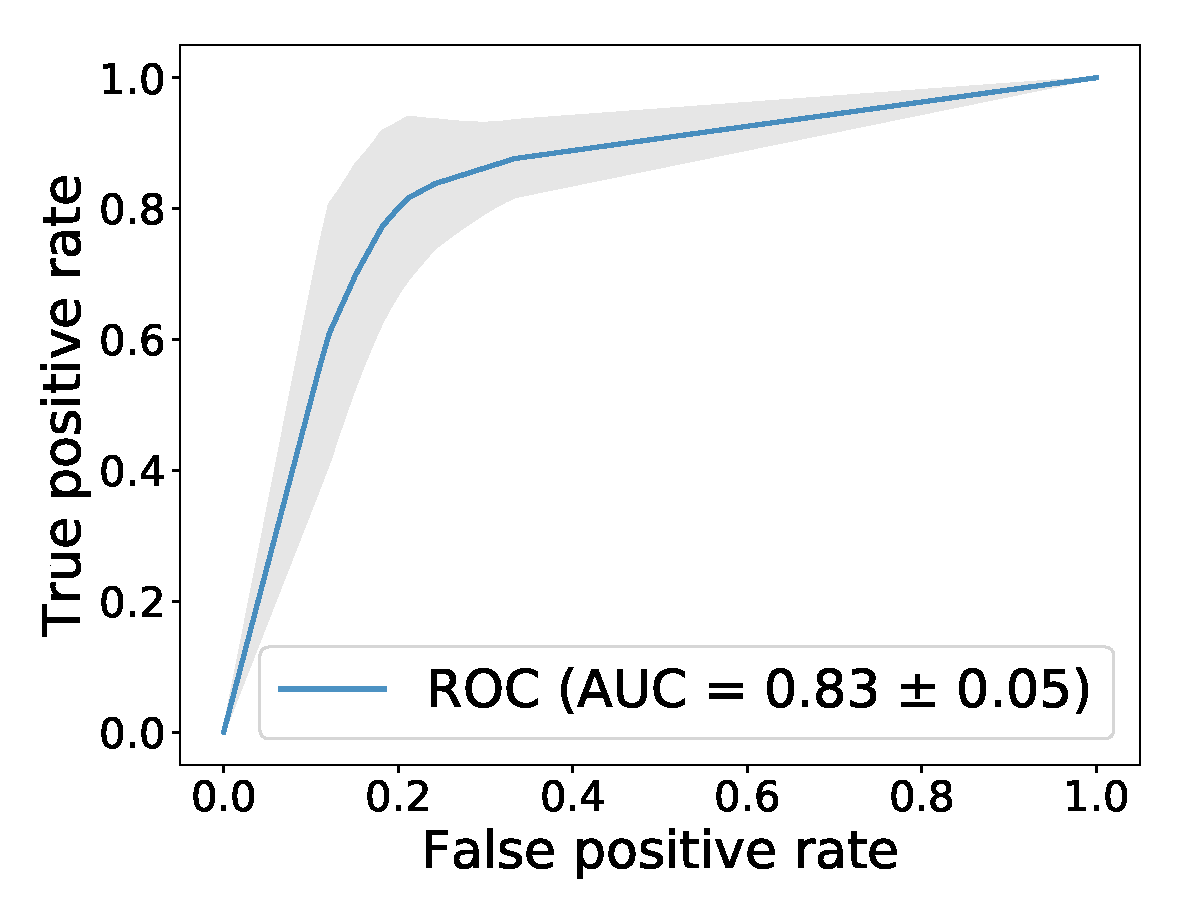
\includegraphics[width=\linewidth]{kfold_10_ntree_1_featmat_base_ech1nb_feat_872019_11_25RF_Source_On_Source_ROC.pdf}\\
        {\small \emph{Source} tested on source}
    \end{minipage}
    \begin{minipage}[t]{\ratio\linewidth}
        \centering
        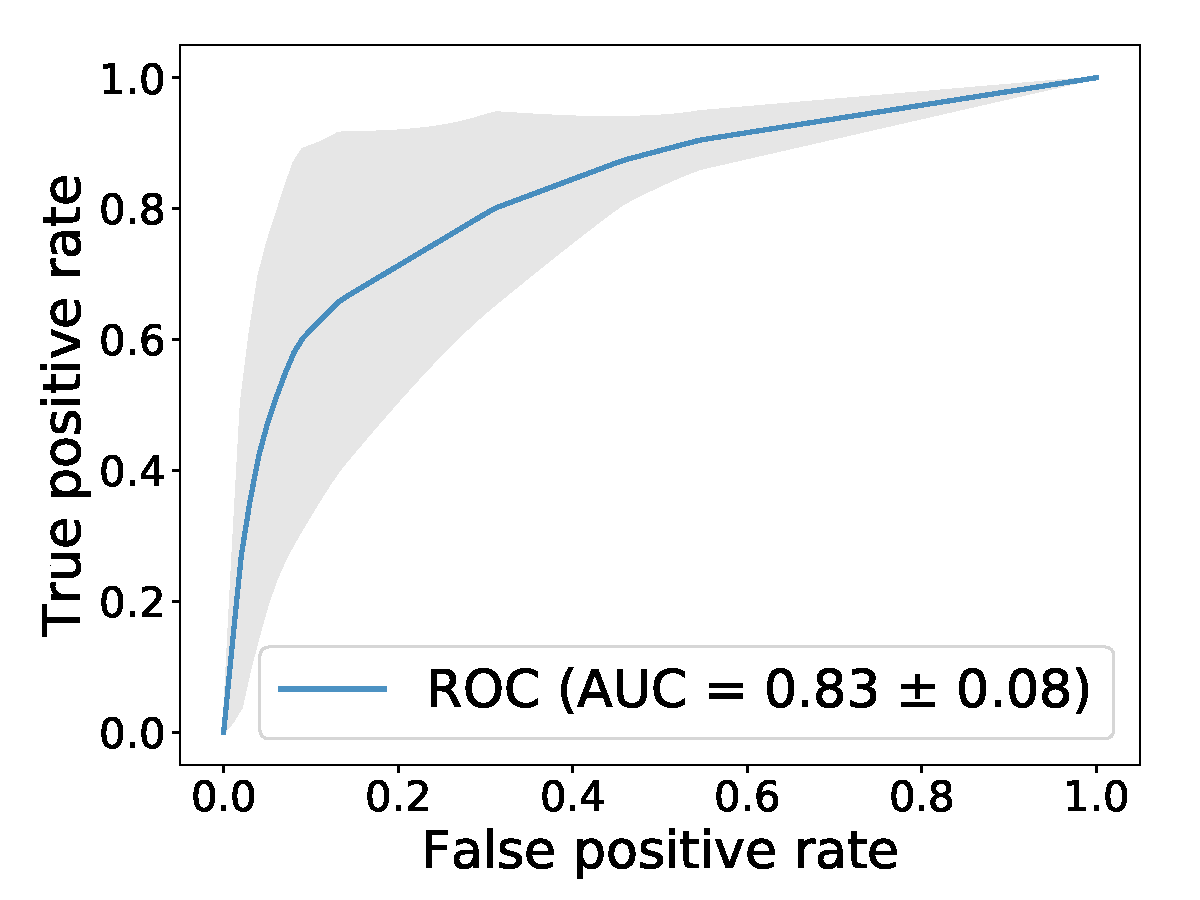
\includegraphics[width=\linewidth]{kfold_10_ntree_1_featmat_base_ech1nb_feat_872019_11_25RF_Source_On_Target_ROC.pdf}\\
        {\small \emph{Source} tested on target}
    \end{minipage}
    \begin{minipage}[t]{\ratio\linewidth}
        \centering
        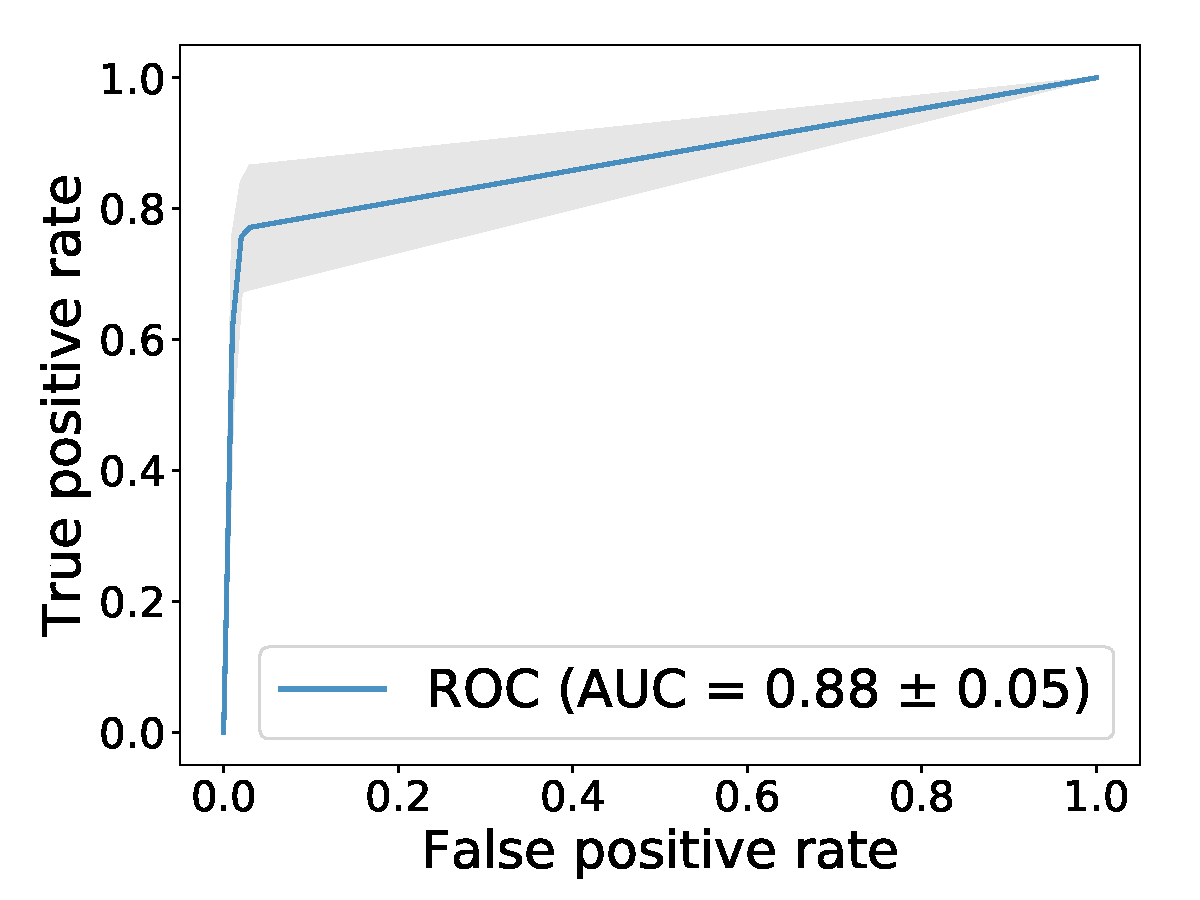
\includegraphics[width=\linewidth]{kfold_10_ntree_1_featmat_base_ech1nb_feat_872019_11_25RF_Target_On_Target_ROC.pdf}\\
        {\small \emph{Target} tested on target}
    \end{minipage}
\end{minipage}

\end{frame}

\begin{frame}{Transfer learning on decision tree}{Model-based transfer}
\begin{minipage}[t]{0.49\linewidth}
    \vspace{0pt}
    \centering
    \textbf{Structure Expansion / Reduction (SER)}
    
    \renewcommand{\ratio}{0.65}
%     \begin{overprint}
%         \onslide<1>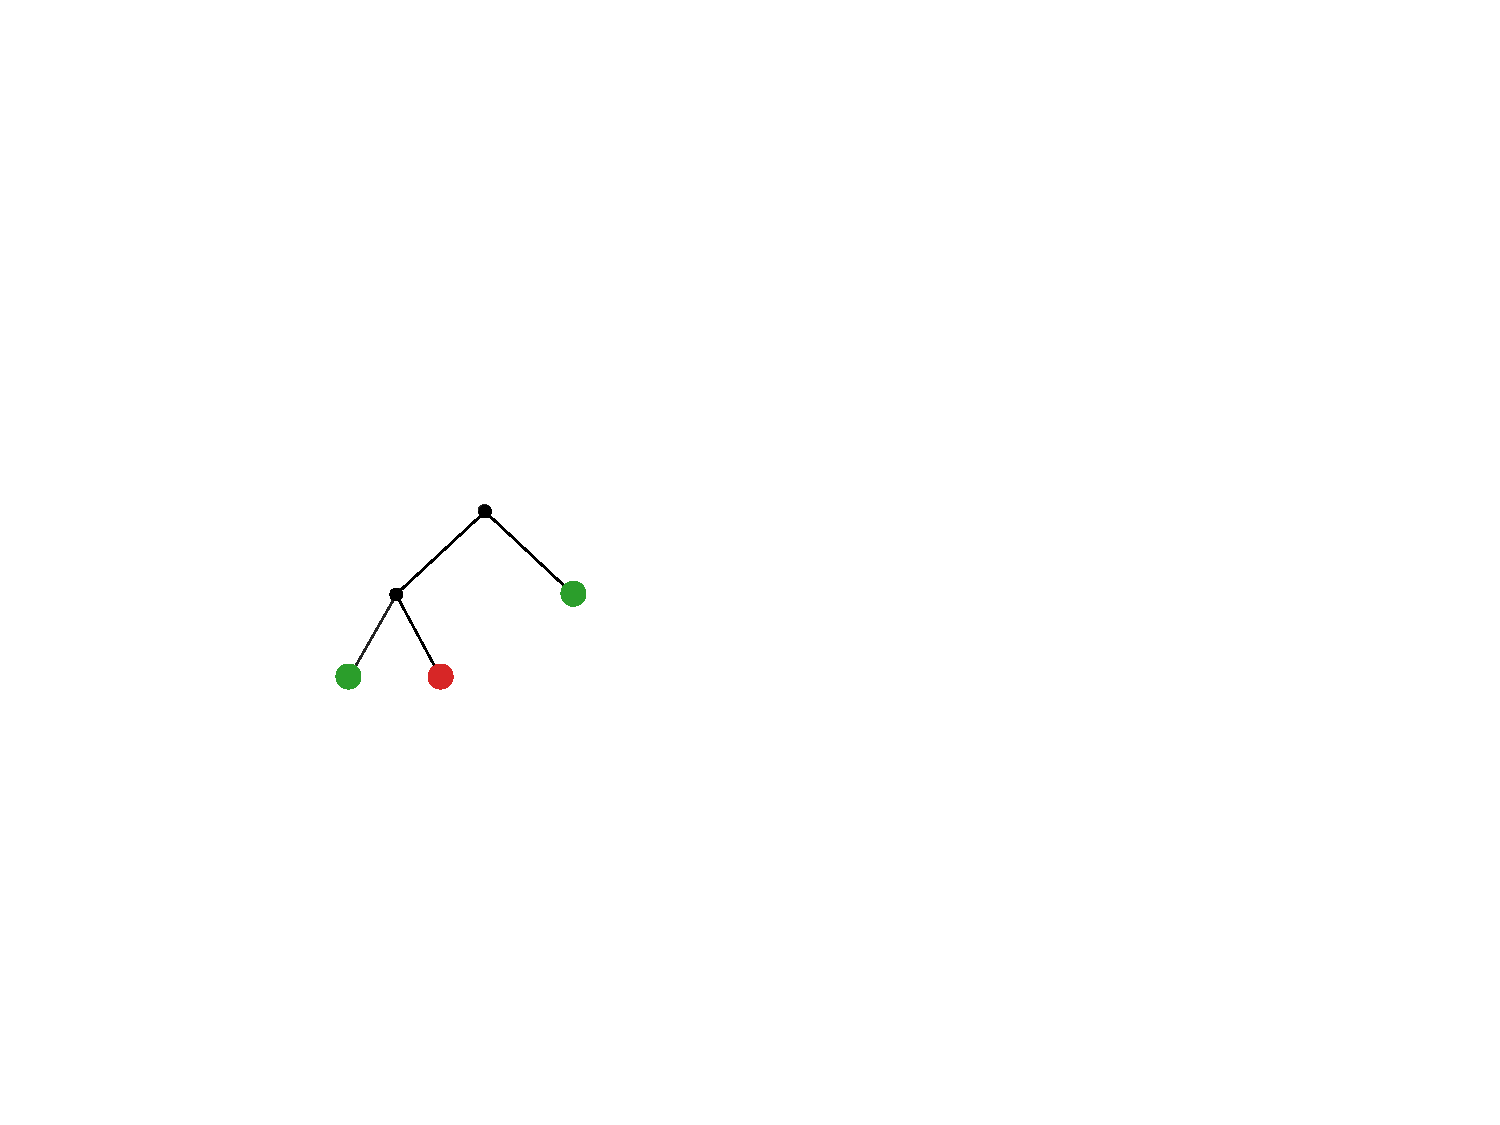
\includegraphics[width=\ratio\linewidth, trim={100 150 430 200}, clip]{ser_0.pdf}
%         \onslide<2>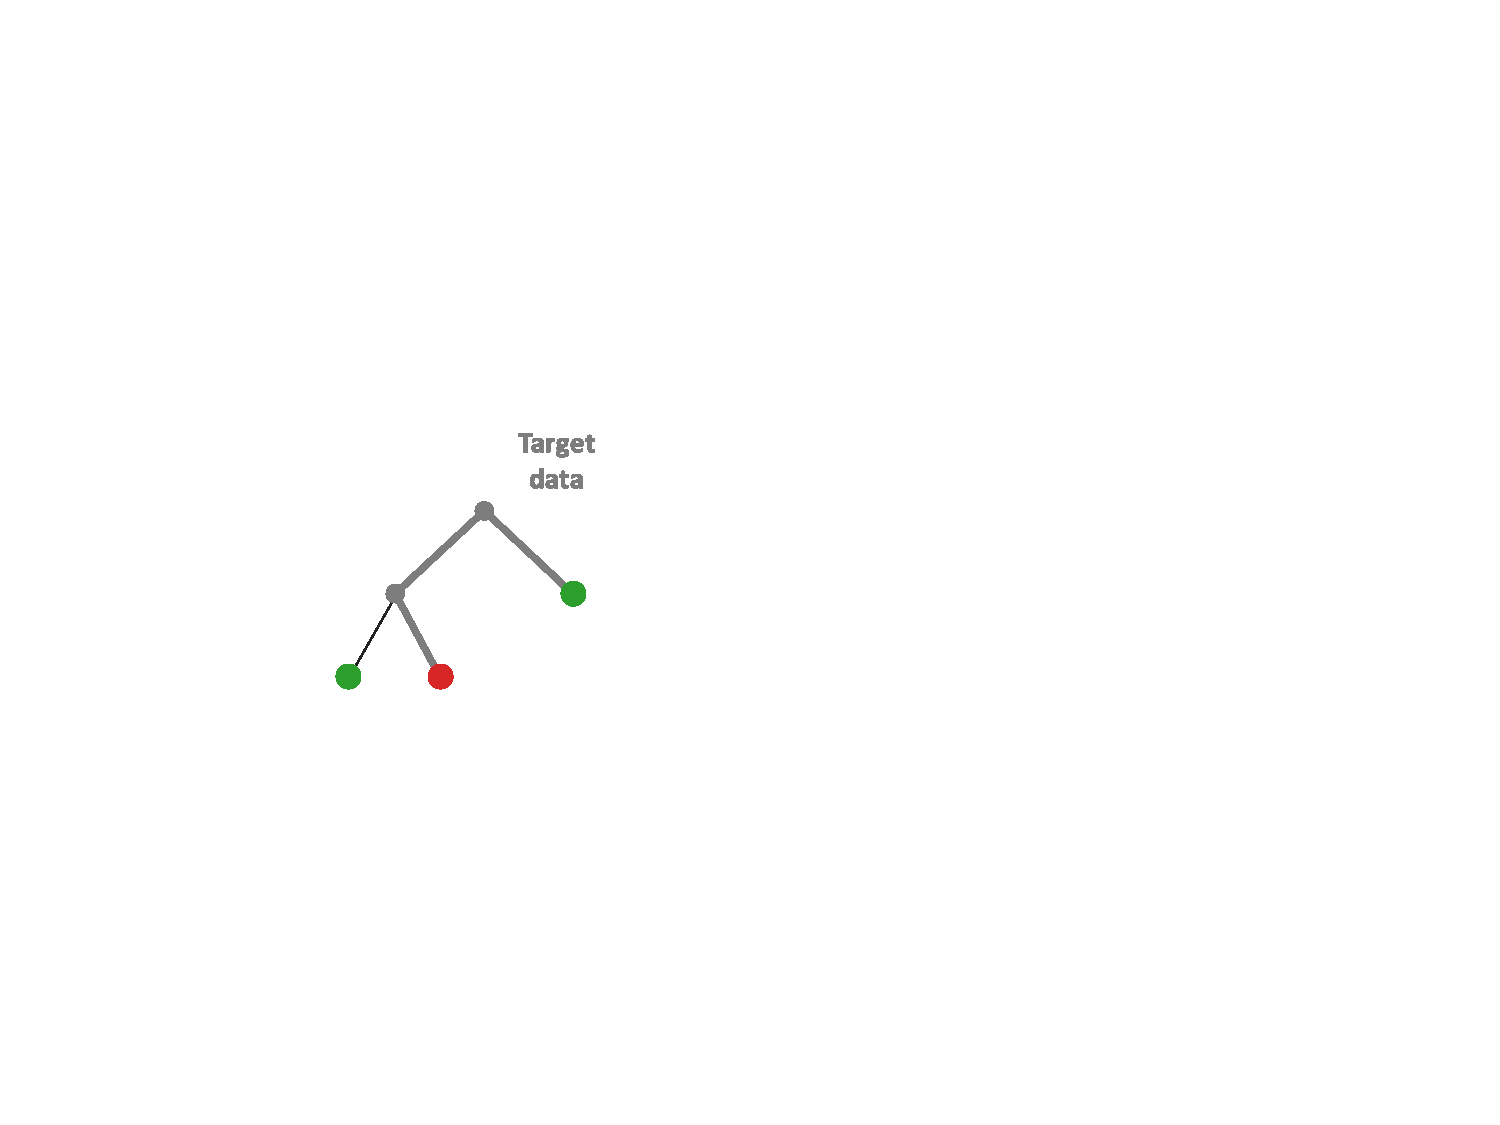
\includegraphics[width=\ratio\linewidth, trim={100 150 430 200}, clip]{ser_1.pdf}
%         \onslide<3>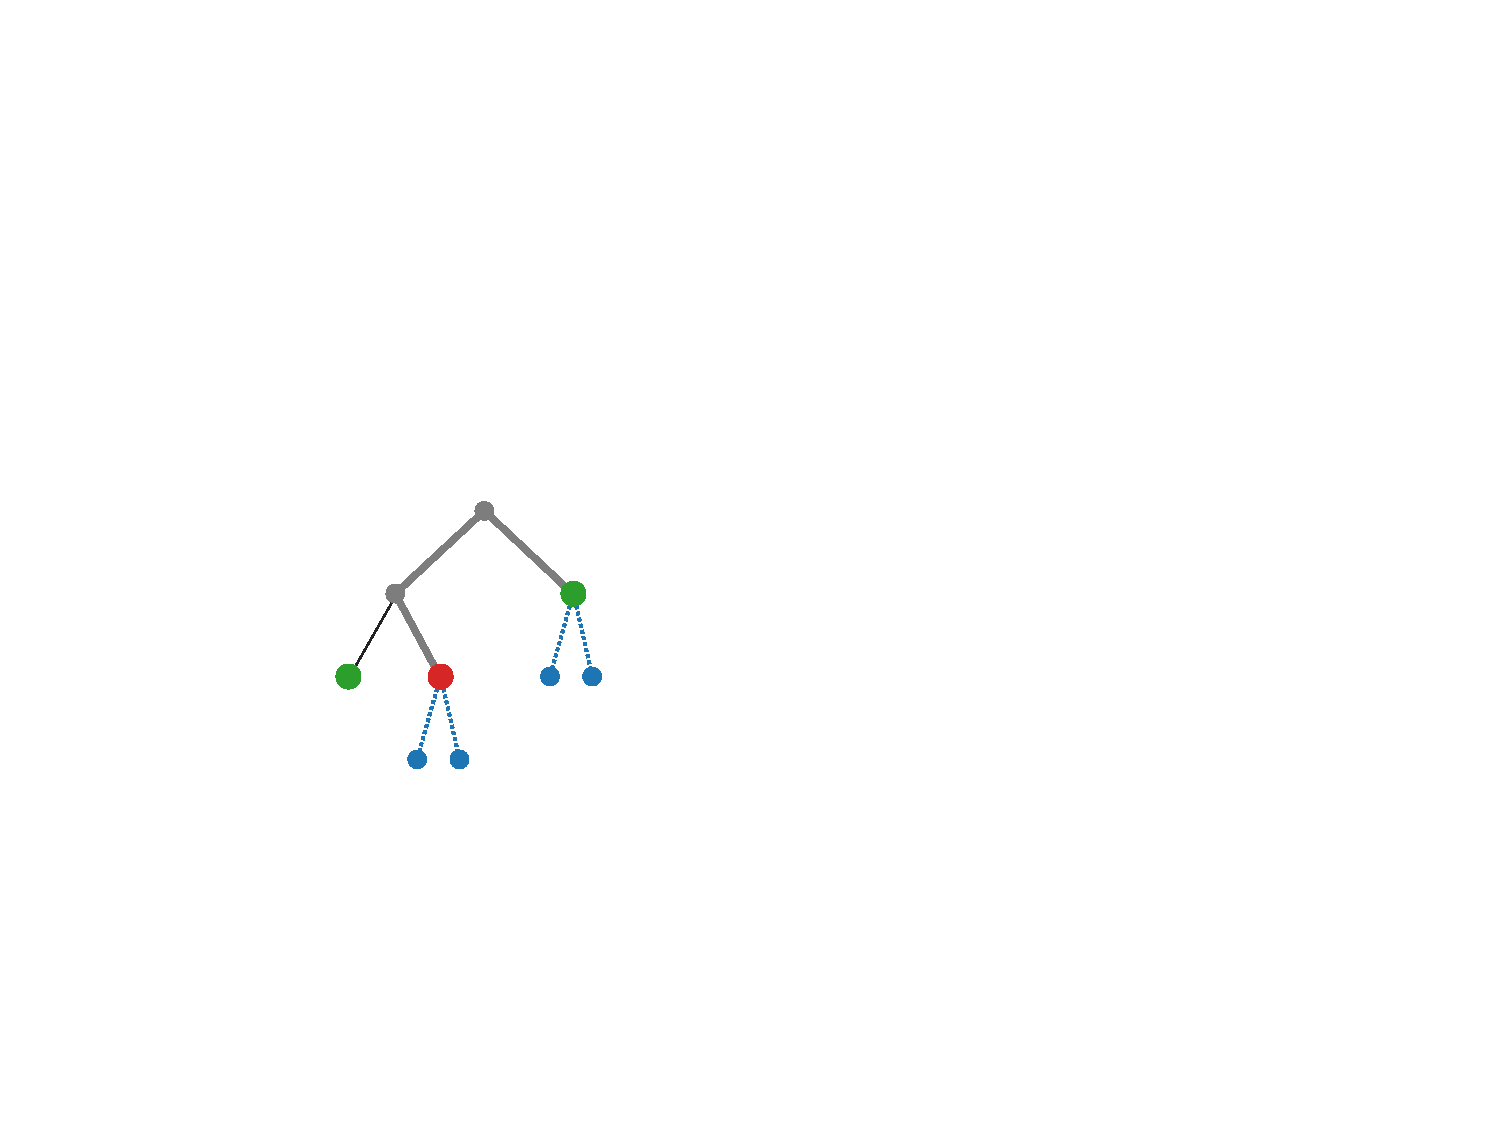
\includegraphics[width=\ratio\linewidth, trim={100 150 430 200}, clip]{ser_2.pdf}
%         \onslide<4>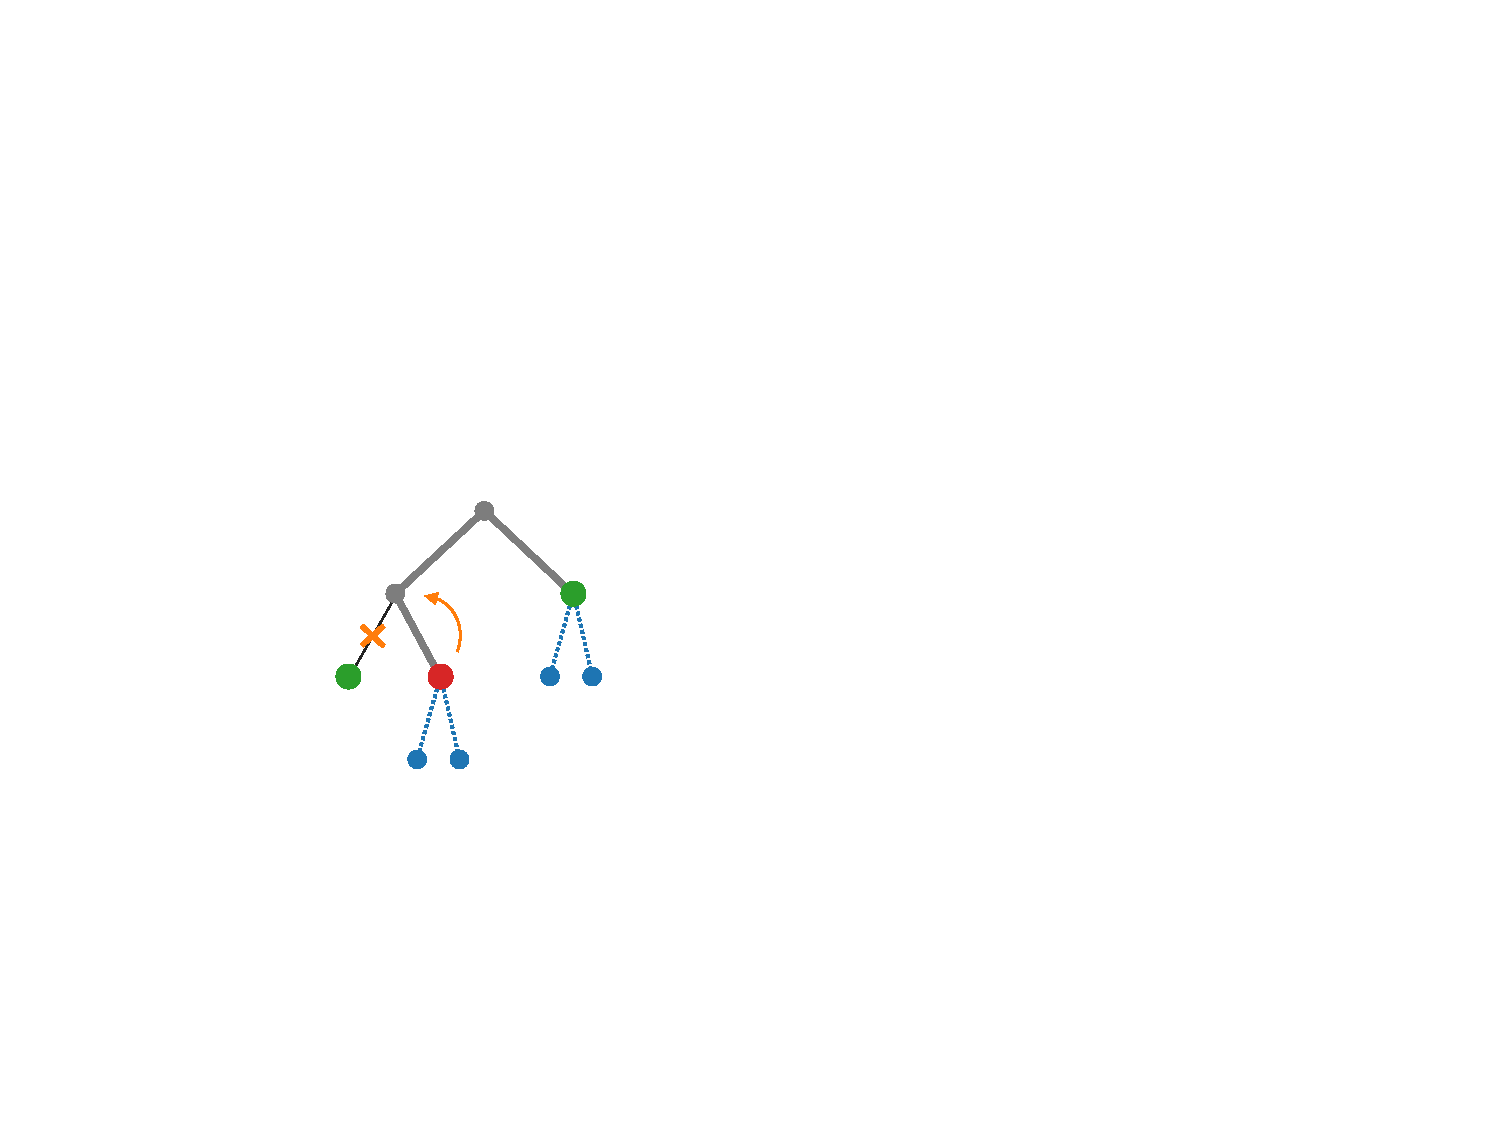
\includegraphics[width=\ratio\linewidth, trim={100 150 430 200}, clip]{ser_3.pdf}
%         \onslide<5->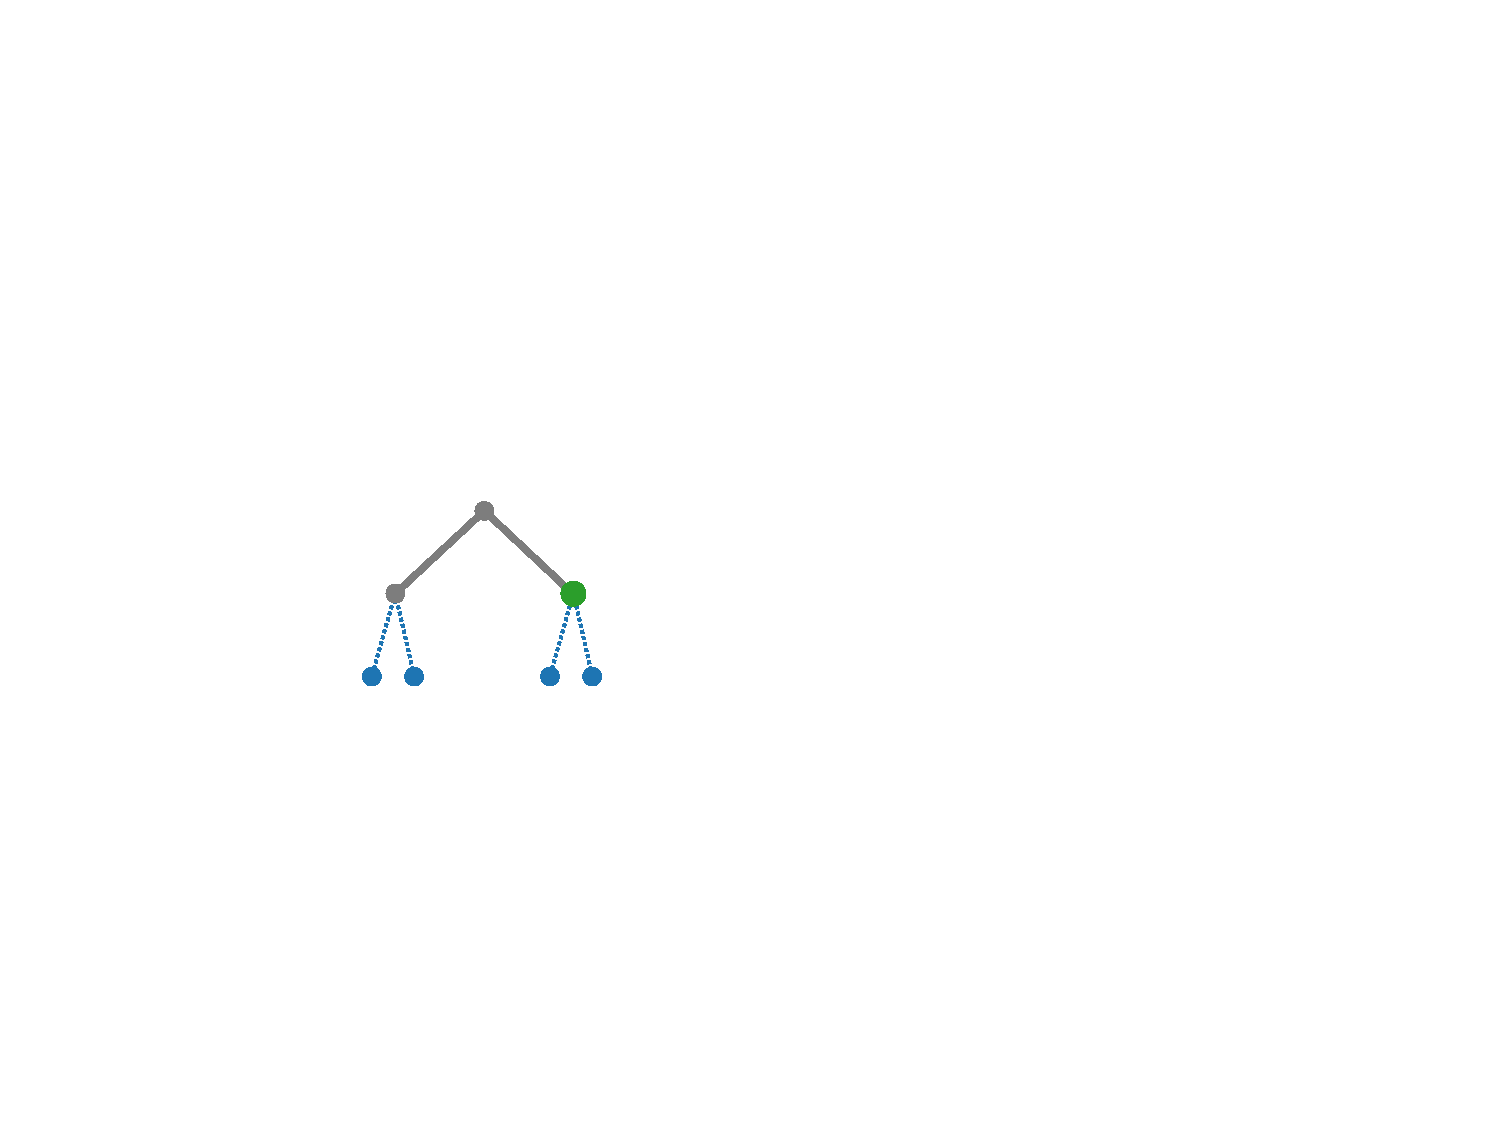
\includegraphics[width=\ratio\linewidth, trim={100 150 430 200}, clip]{ser_4.pdf}
%     \end{overprint}
    \begin{overprint}
        \onslide<1>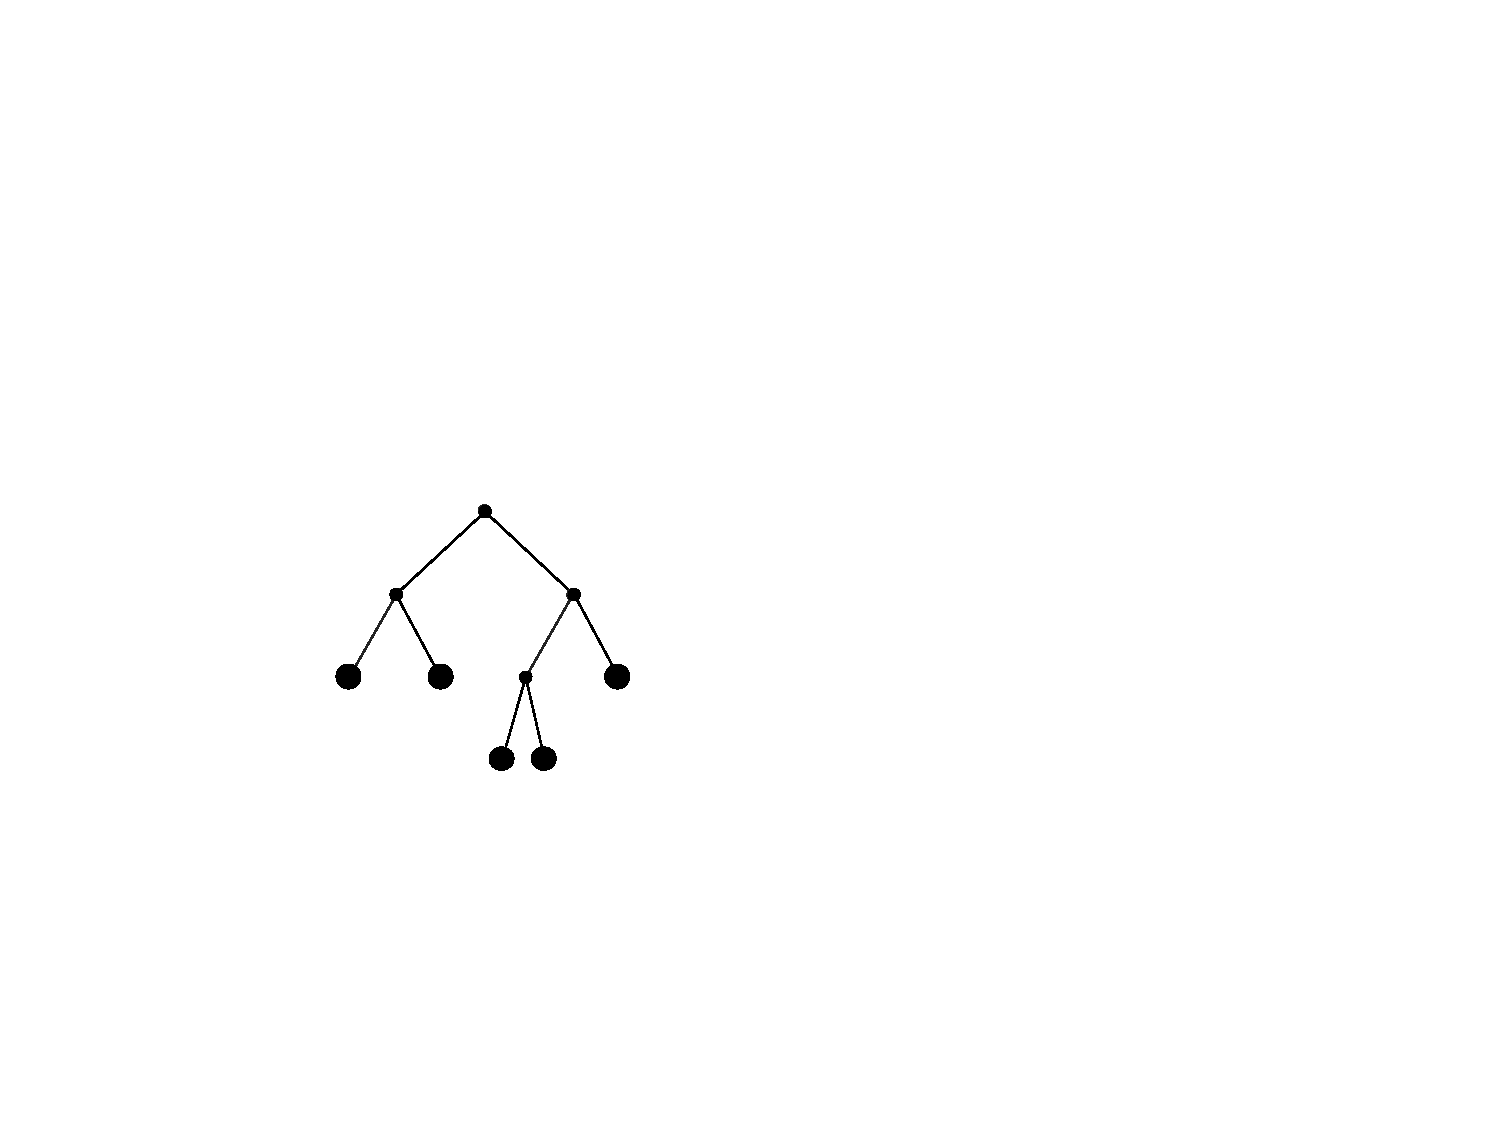
\includegraphics[width=\ratio\linewidth, trim={100 150 430 200}, clip]{schemas_ser_1.pdf}
        \onslide<2>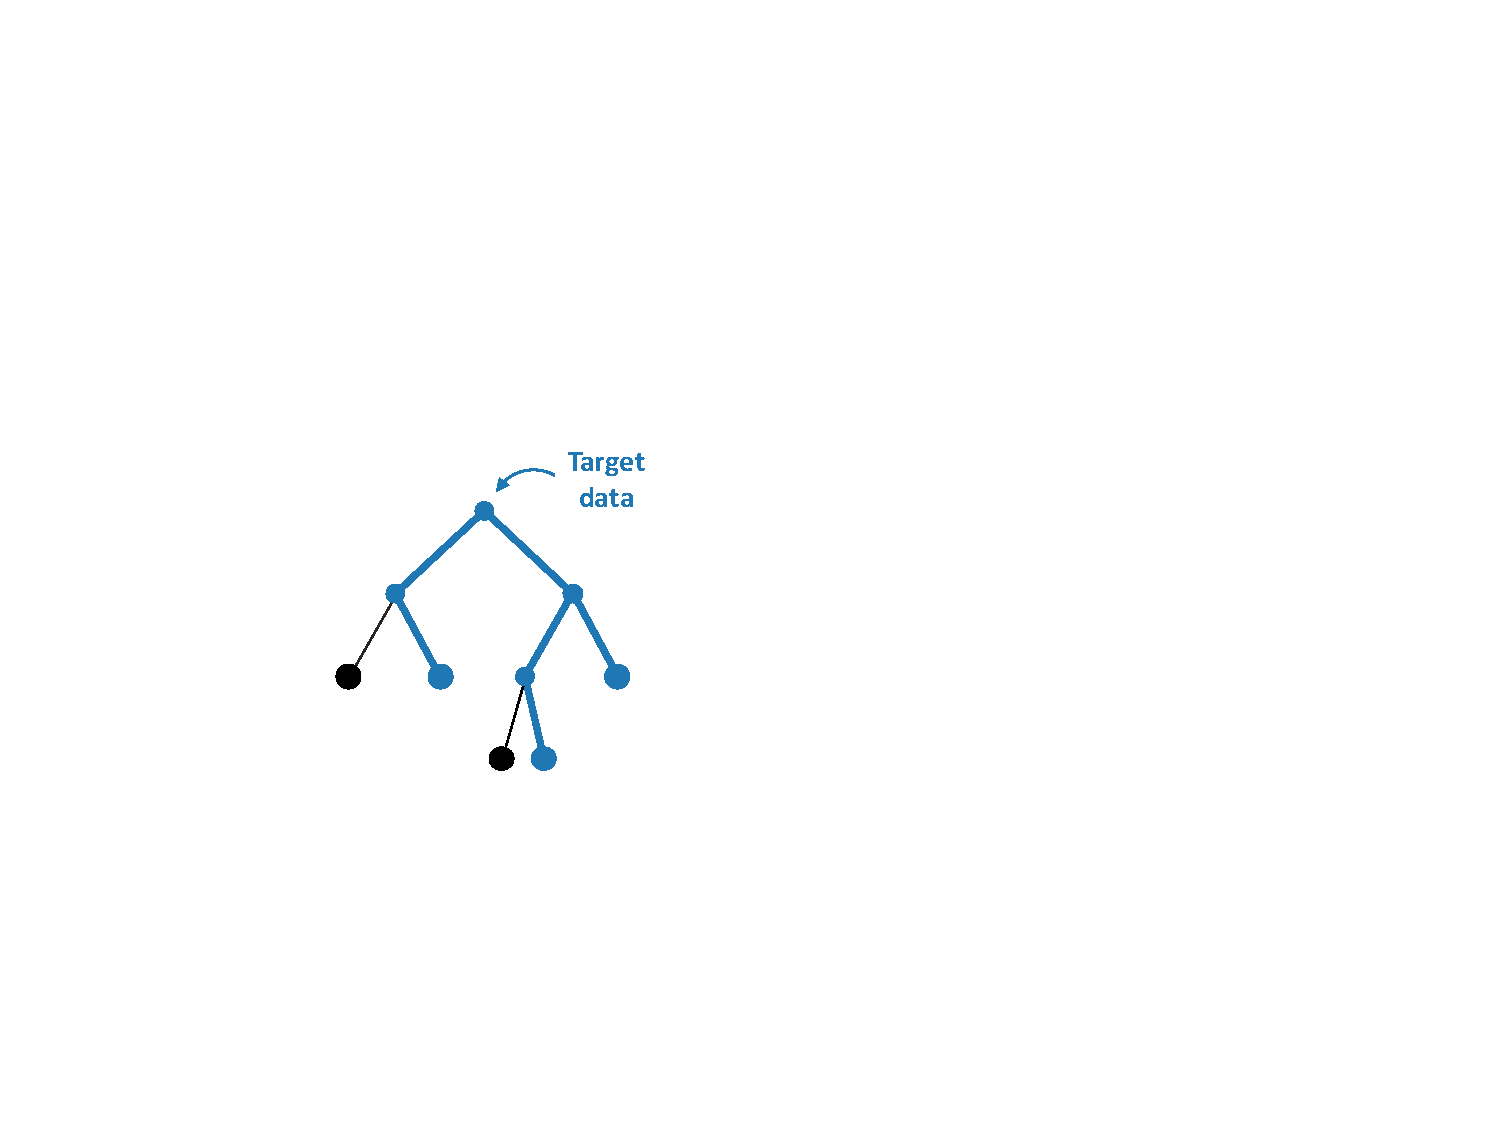
\includegraphics[width=\ratio\linewidth, trim={100 150 430 200}, clip]{schemas_ser_2.pdf}
        \onslide<3>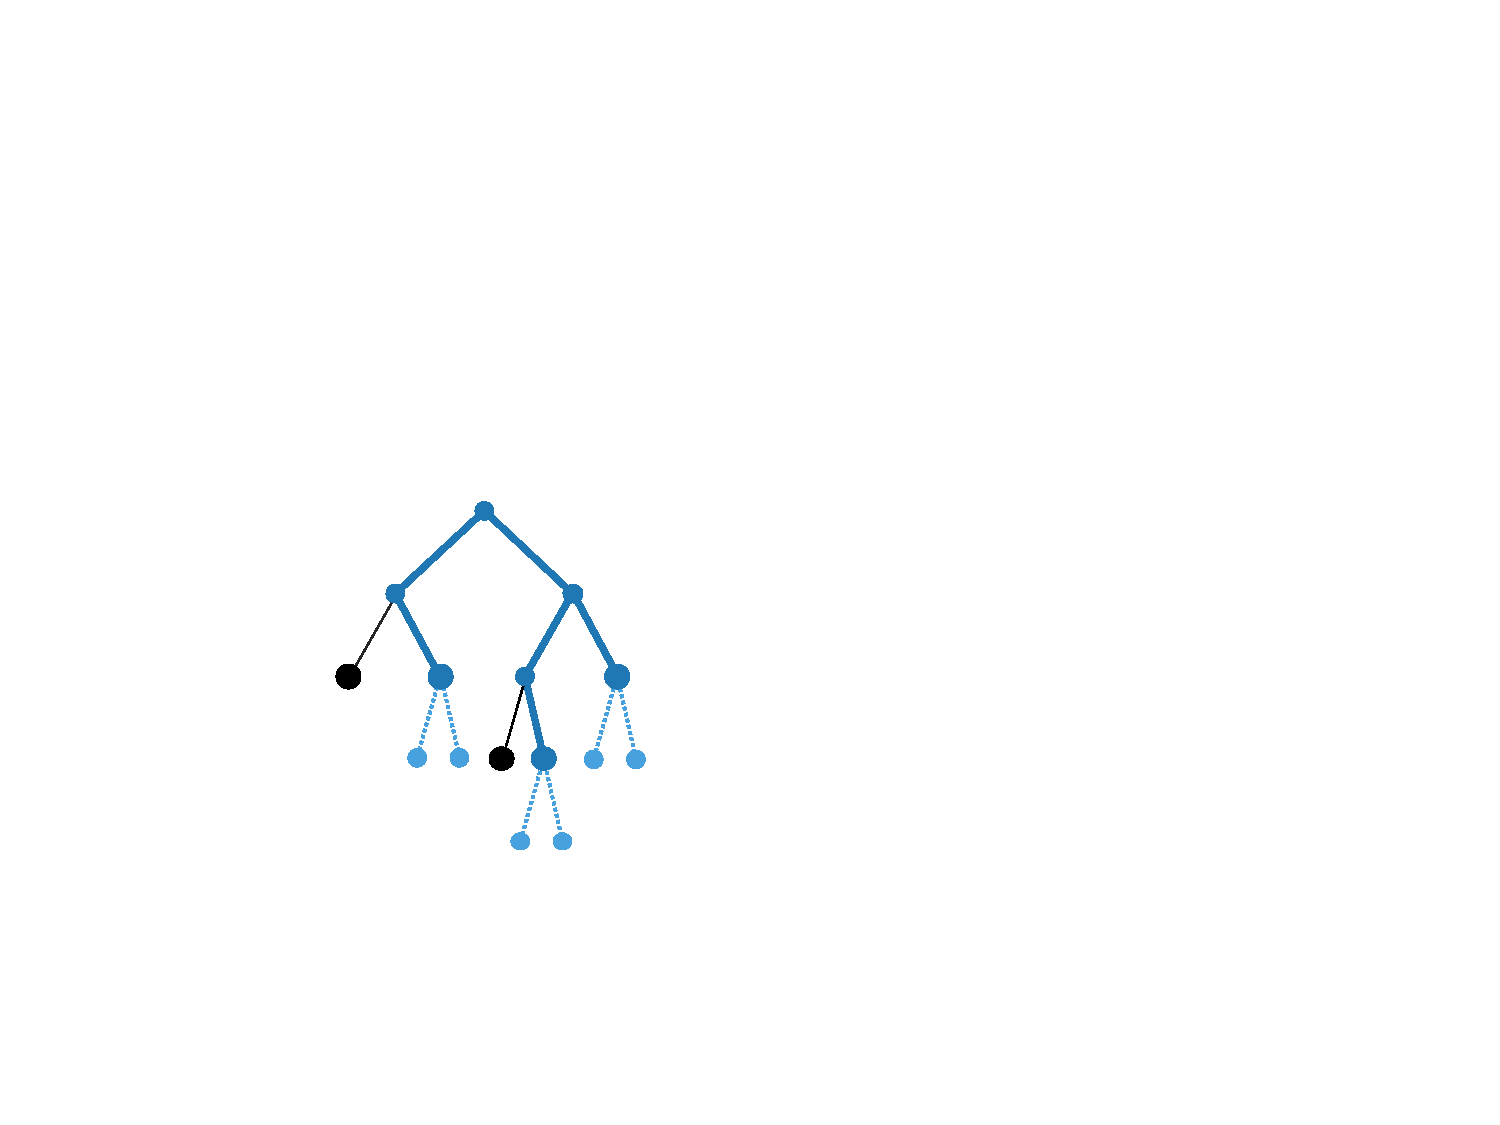
\includegraphics[width=\ratio\linewidth, trim={100 150 430 200}, clip]{schemas_ser_3.pdf}
        \onslide<4>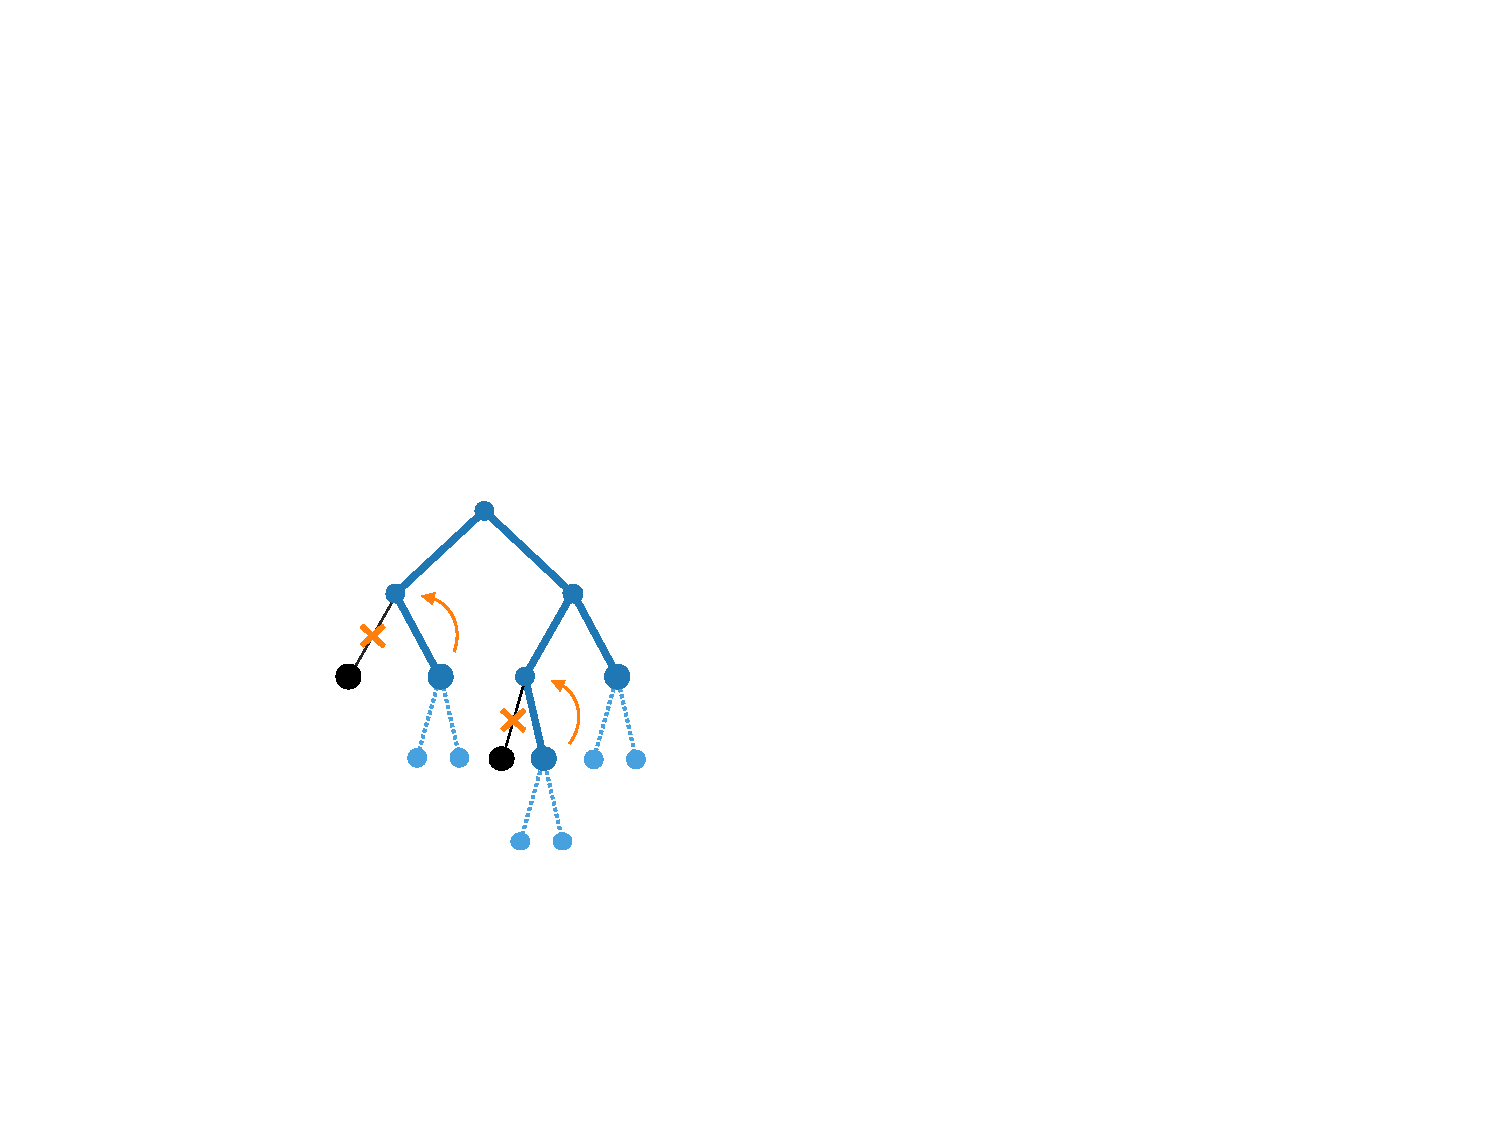
\includegraphics[width=\ratio\linewidth, trim={100 150 430 200}, clip]{schemas_ser_4.pdf}
        \onslide<5->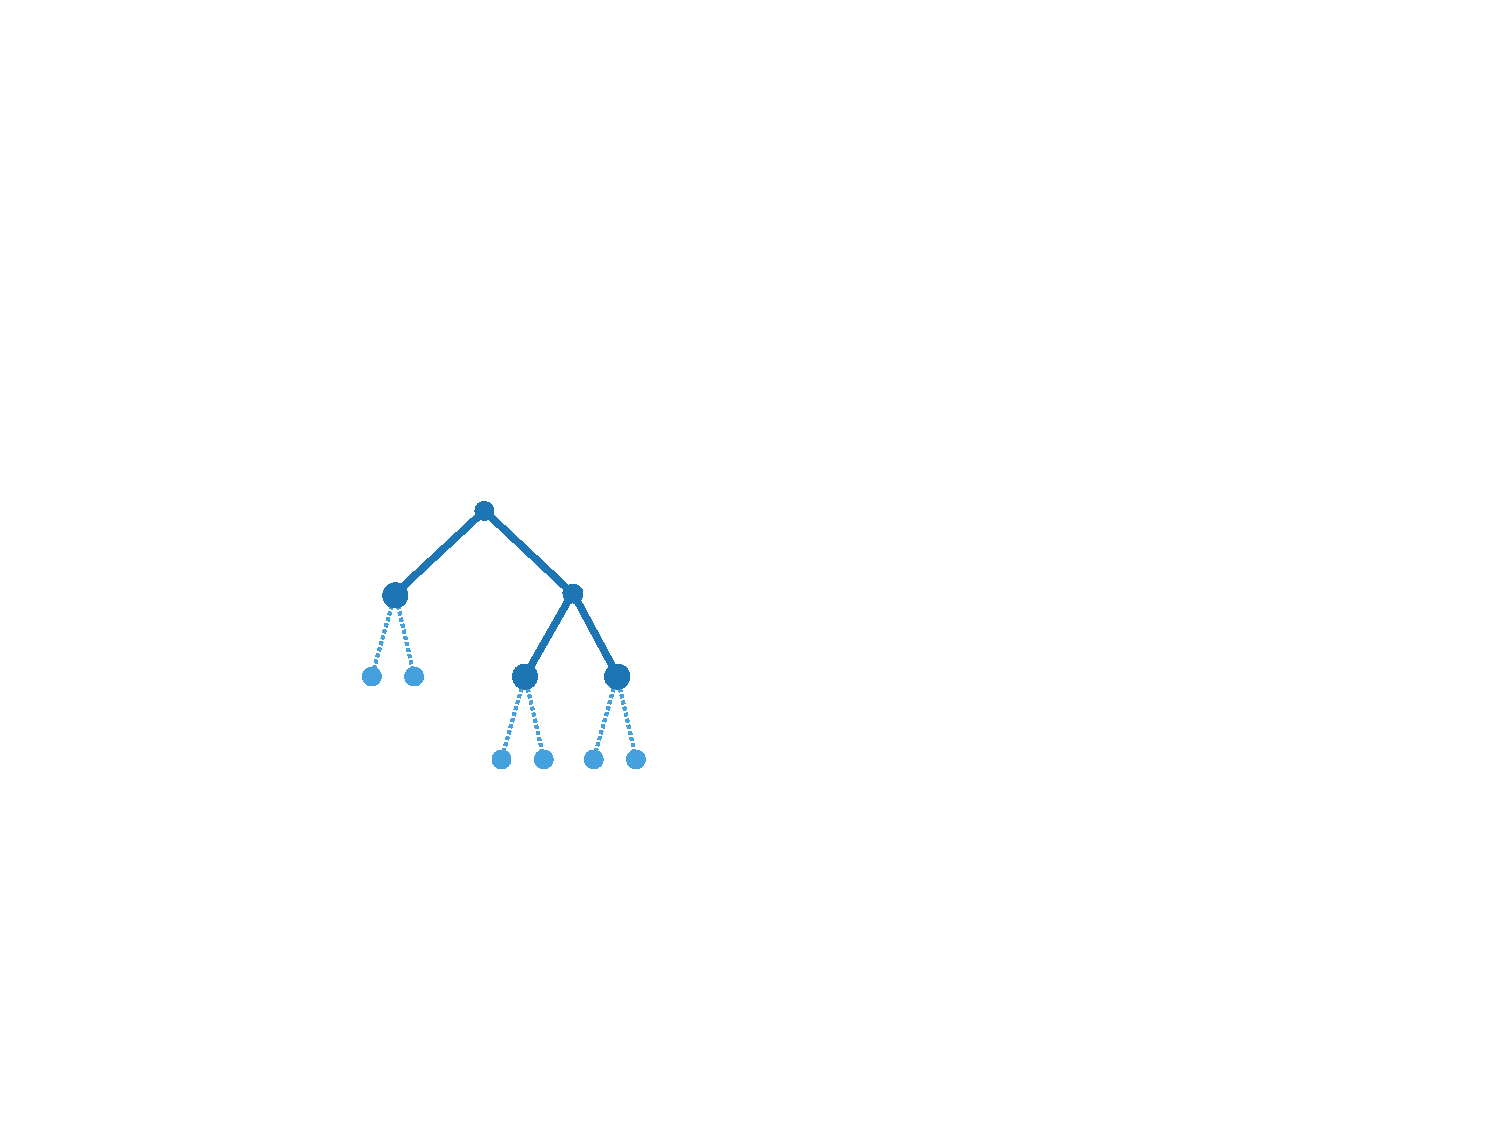
\includegraphics[width=\ratio\linewidth, trim={100 150 430 200}, clip]{schemas_ser_5.pdf}
    \end{overprint}
    
    \textcolor{myblue}{1. Expansion}\\
    \textcolor{myorange}{2. Reduction}\\
    Partition refinement or simplification

\end{minipage}\hfill
\begin{minipage}[t]{0.49\linewidth}
    \vspace{0pt}
    \centering
    \textbf{Structure Transfer}
    
    \renewcommand{\ratio}{0.65}
%     \begin{overprint}
%         \onslide<6>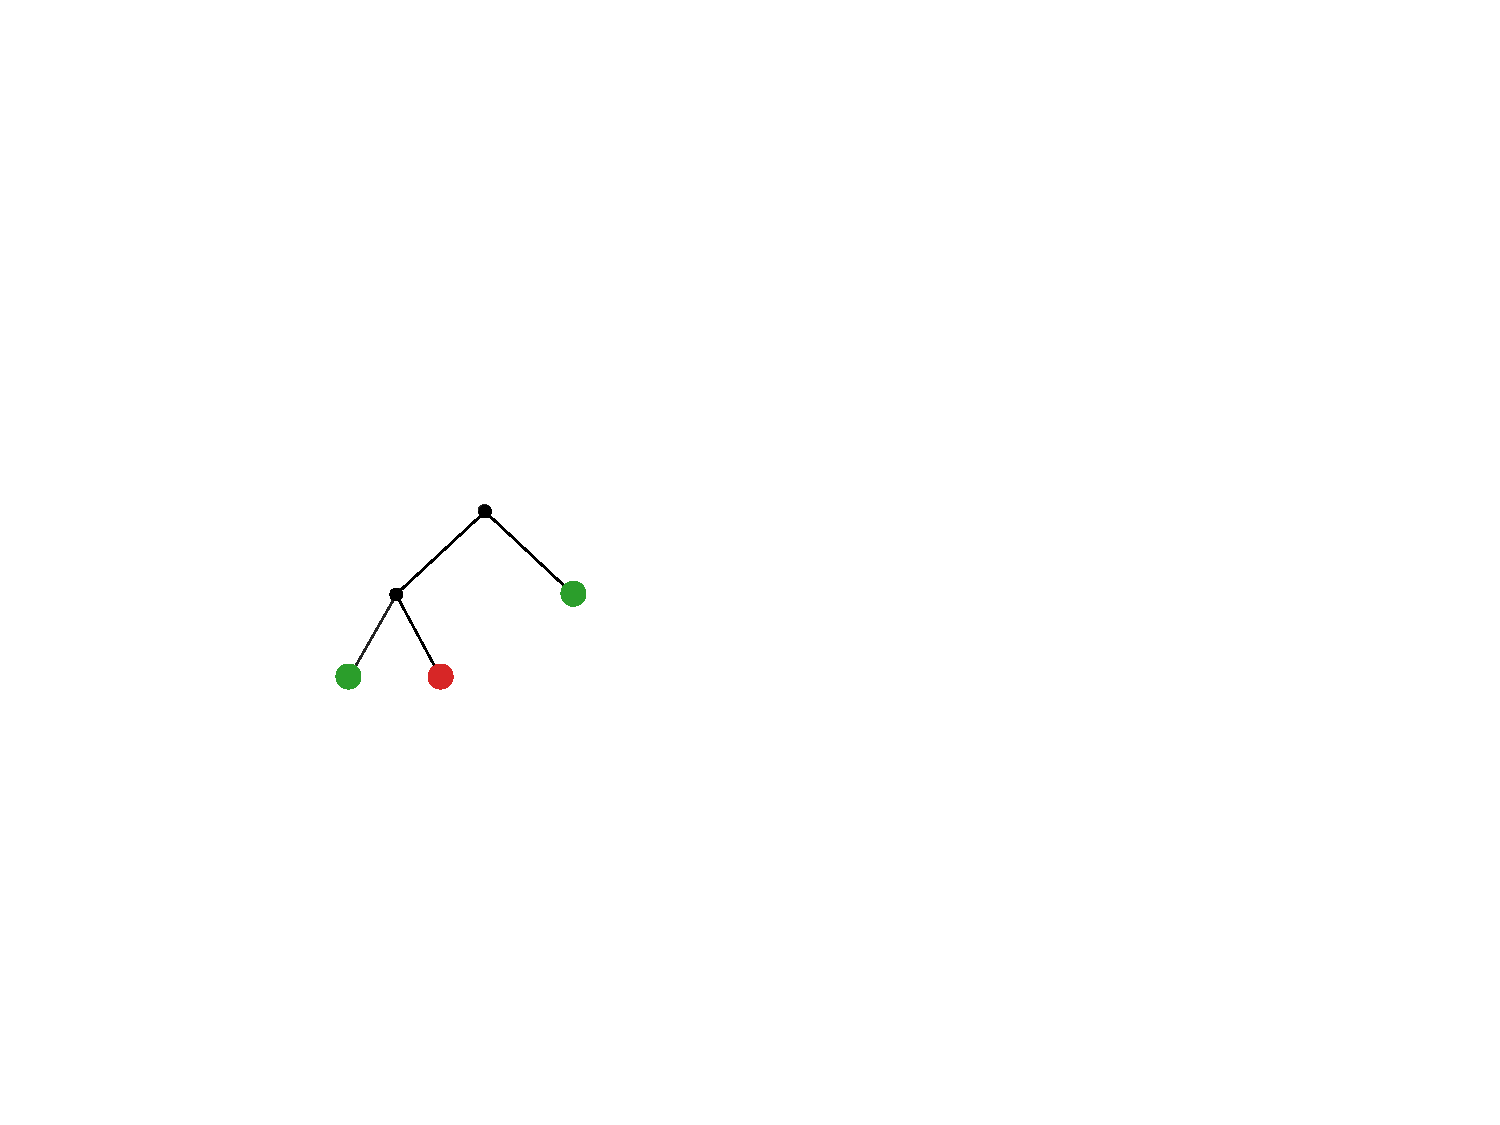
\includegraphics[width=\ratio\linewidth, trim={100 180 430 200}, clip]{strut_0.pdf}
%         \onslide<7>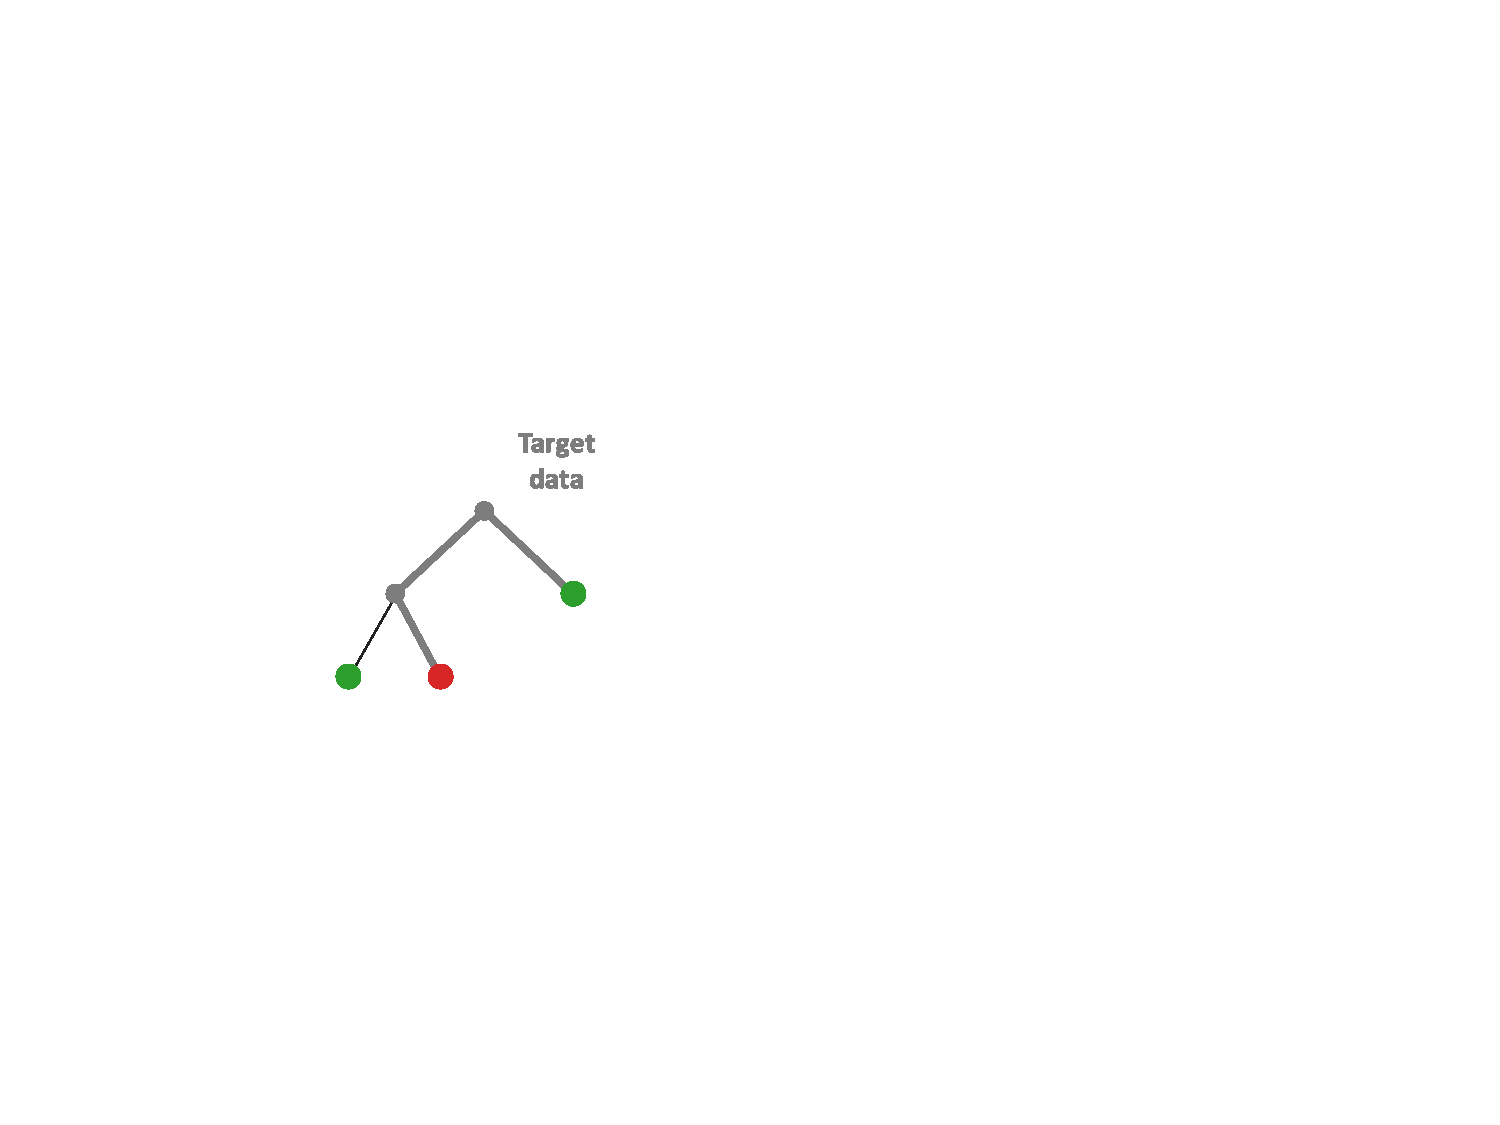
\includegraphics[width=\ratio\linewidth, trim={100 180 430 200}, clip]{strut_1.pdf}
%         \onslide<8>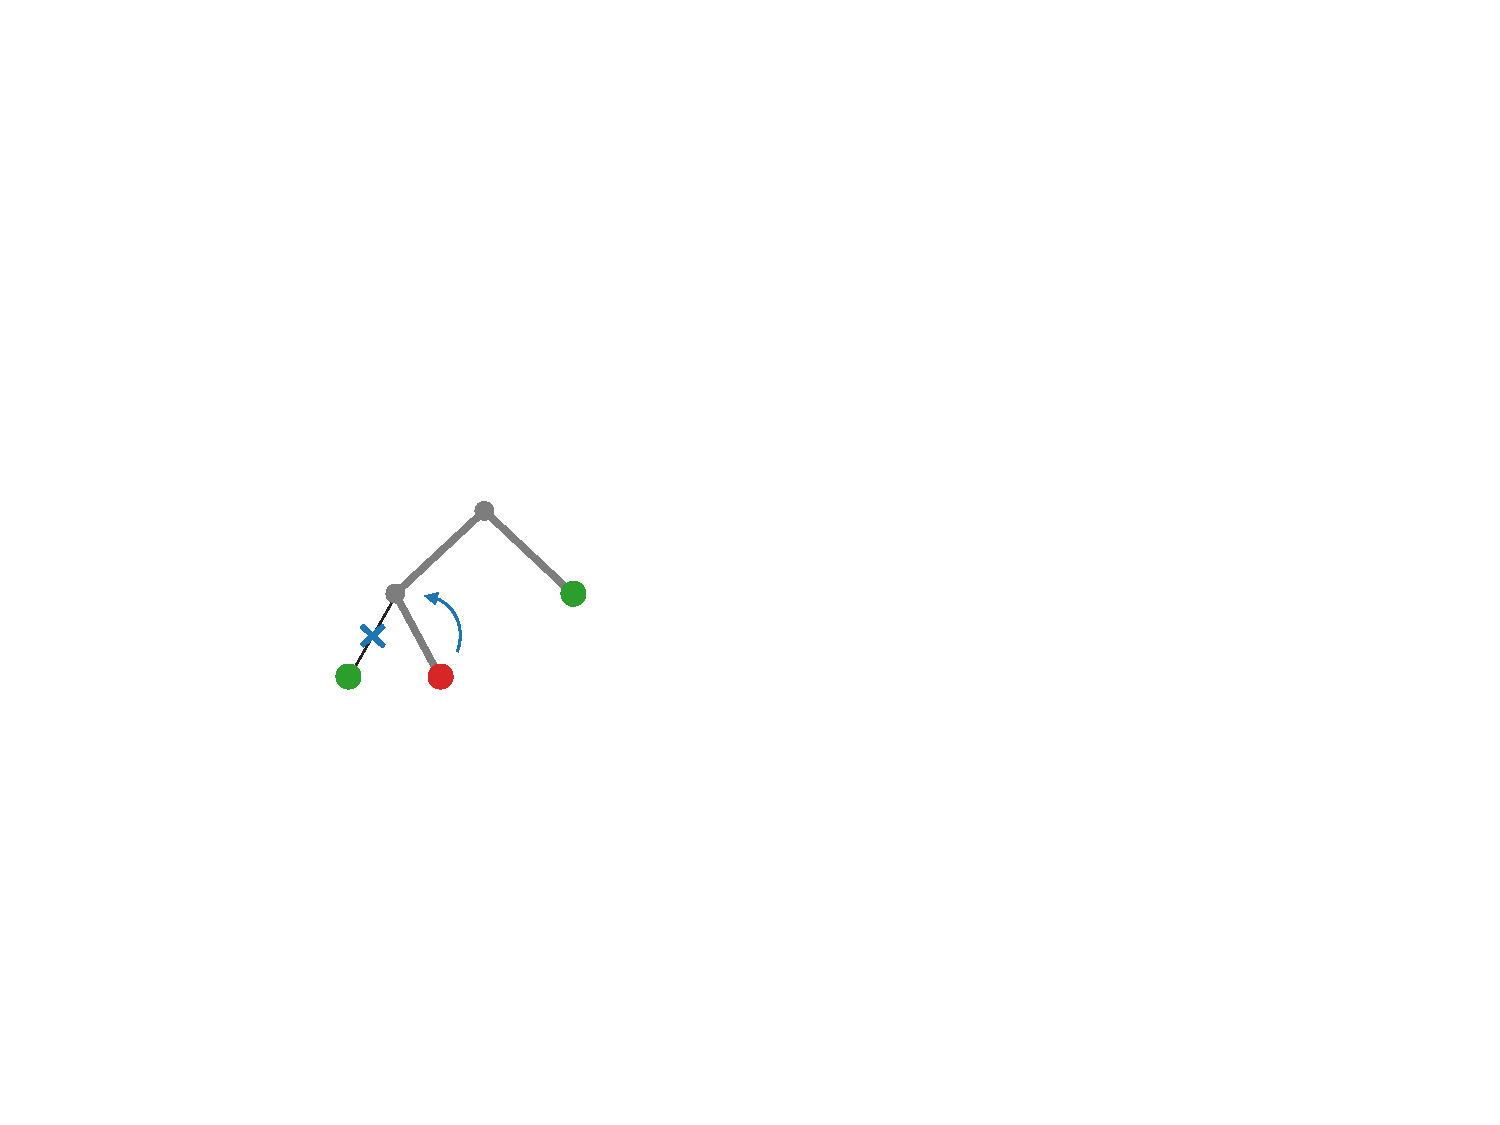
\includegraphics[width=\ratio\linewidth, trim={100 180 430 200}, clip]{strut_2.pdf}
%         \onslide<9>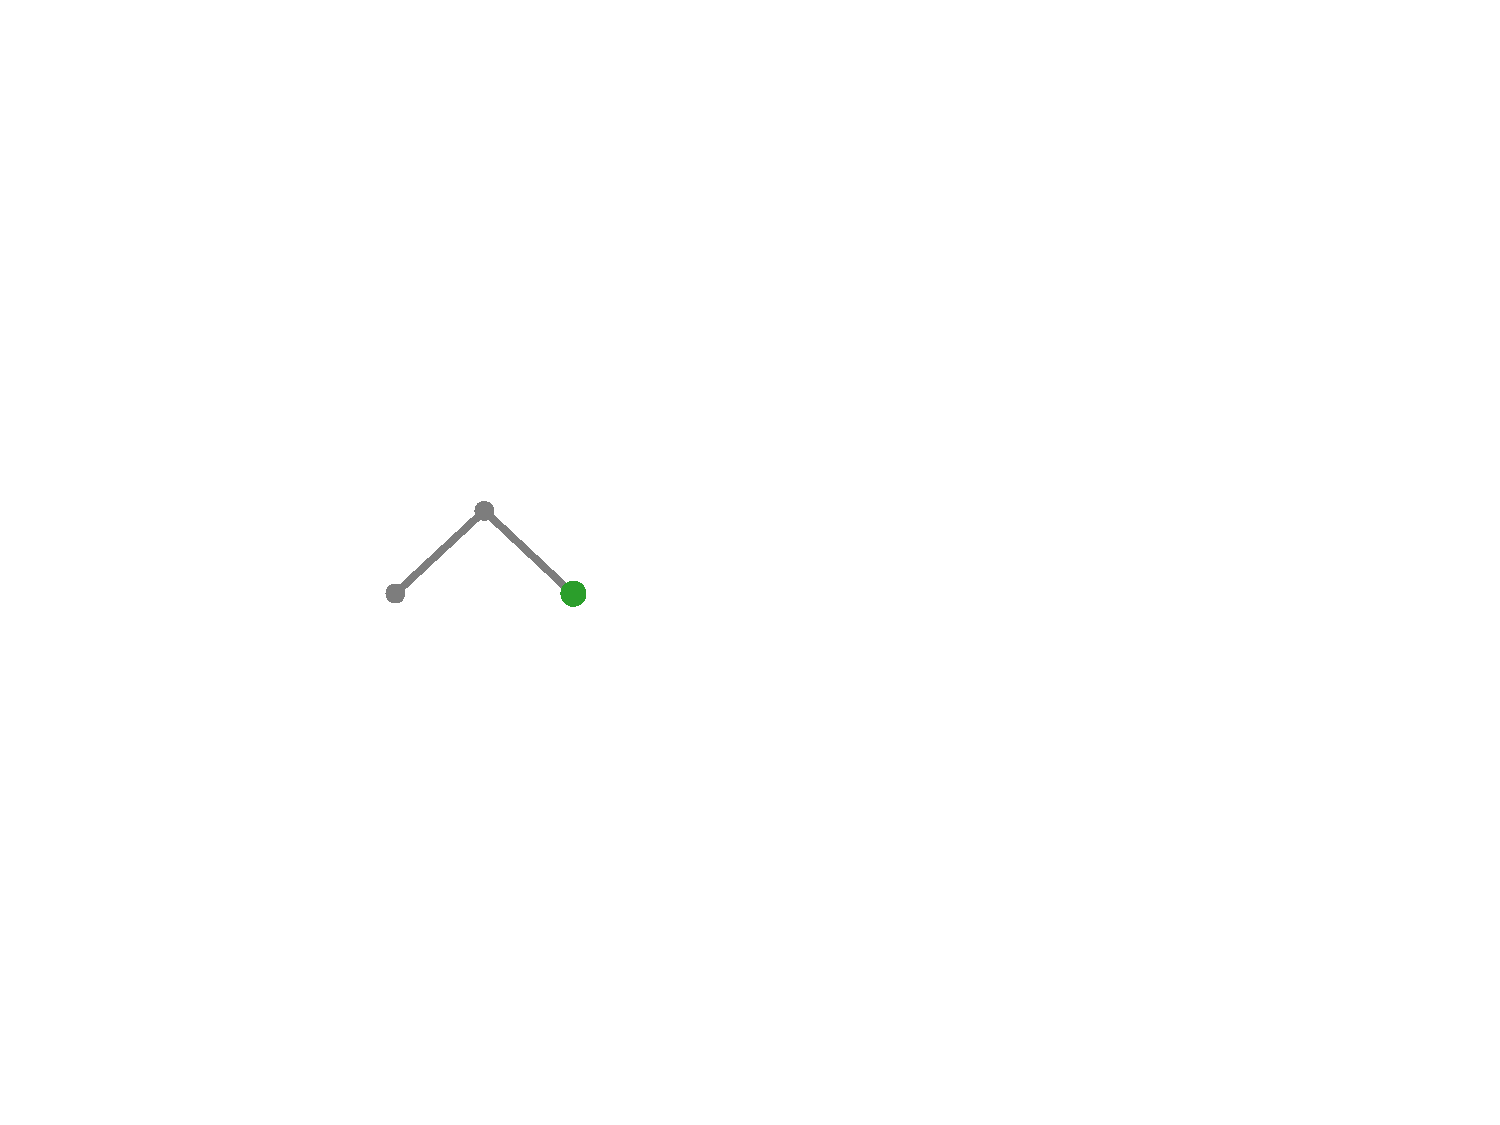
\includegraphics[width=\ratio\linewidth, trim={100 180 430 200}, clip]{strut_3.pdf}
%         \onslide<10->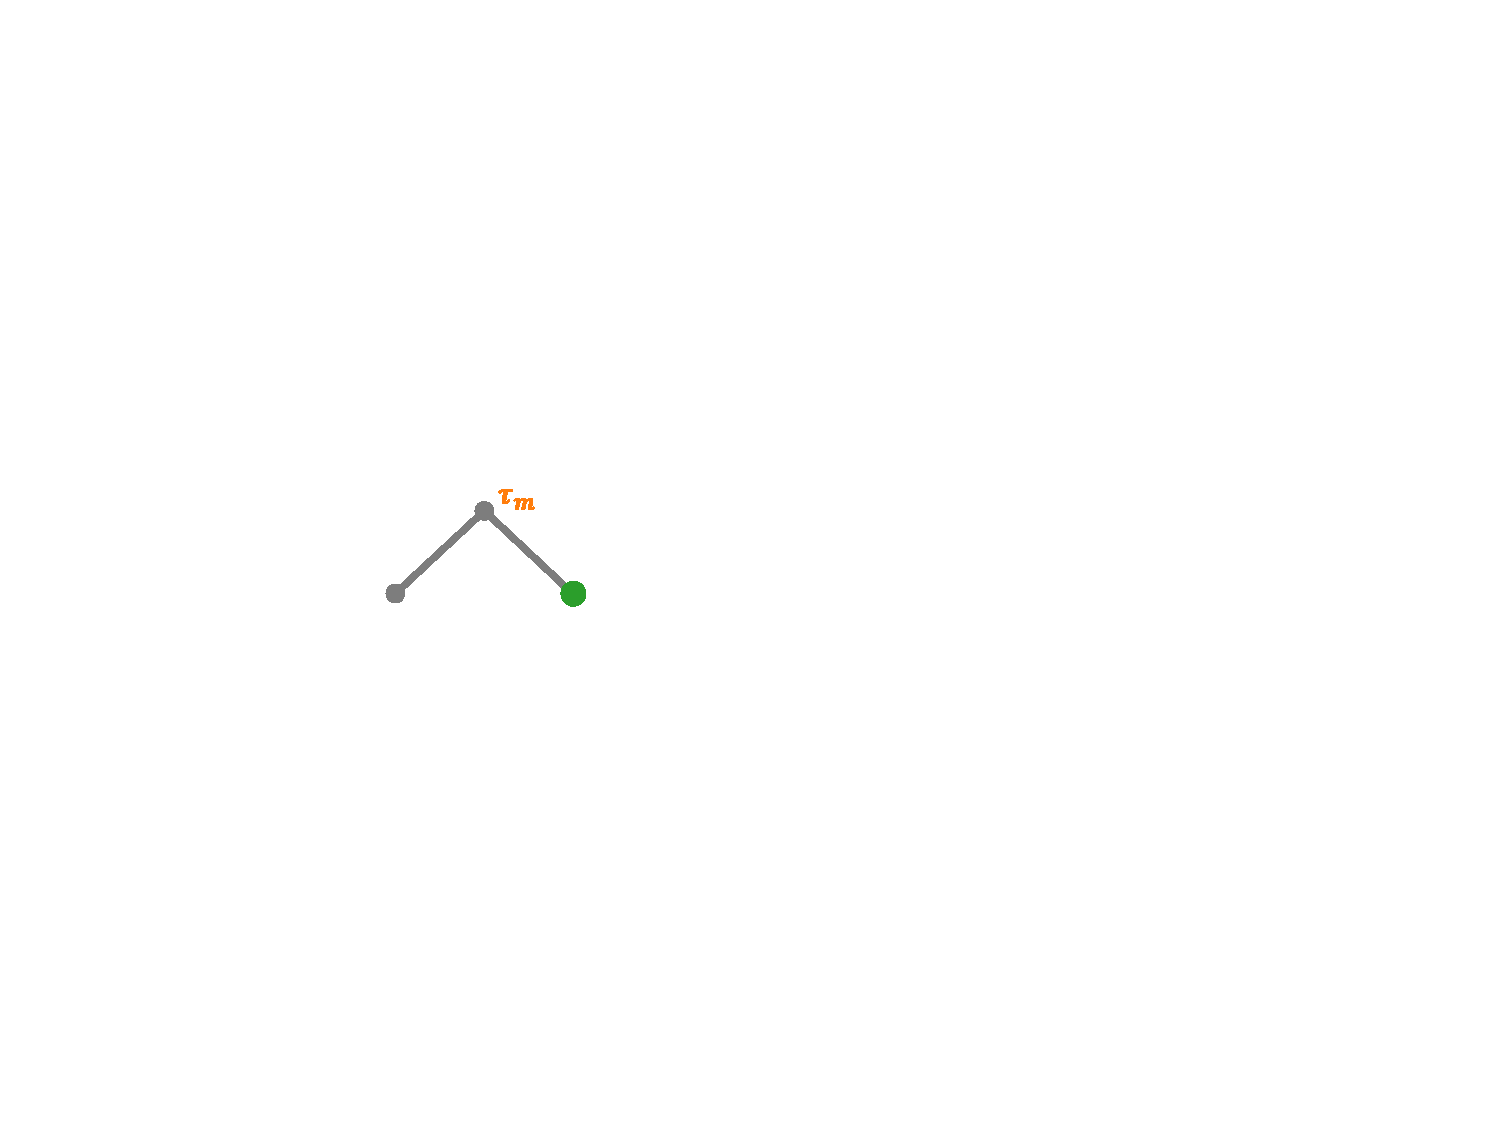
\includegraphics[width=\ratio\linewidth, trim={100 180 430 200}, clip]{strut_4.pdf}
%     \end{overprint}
    \begin{overprint}
        \onslide<6>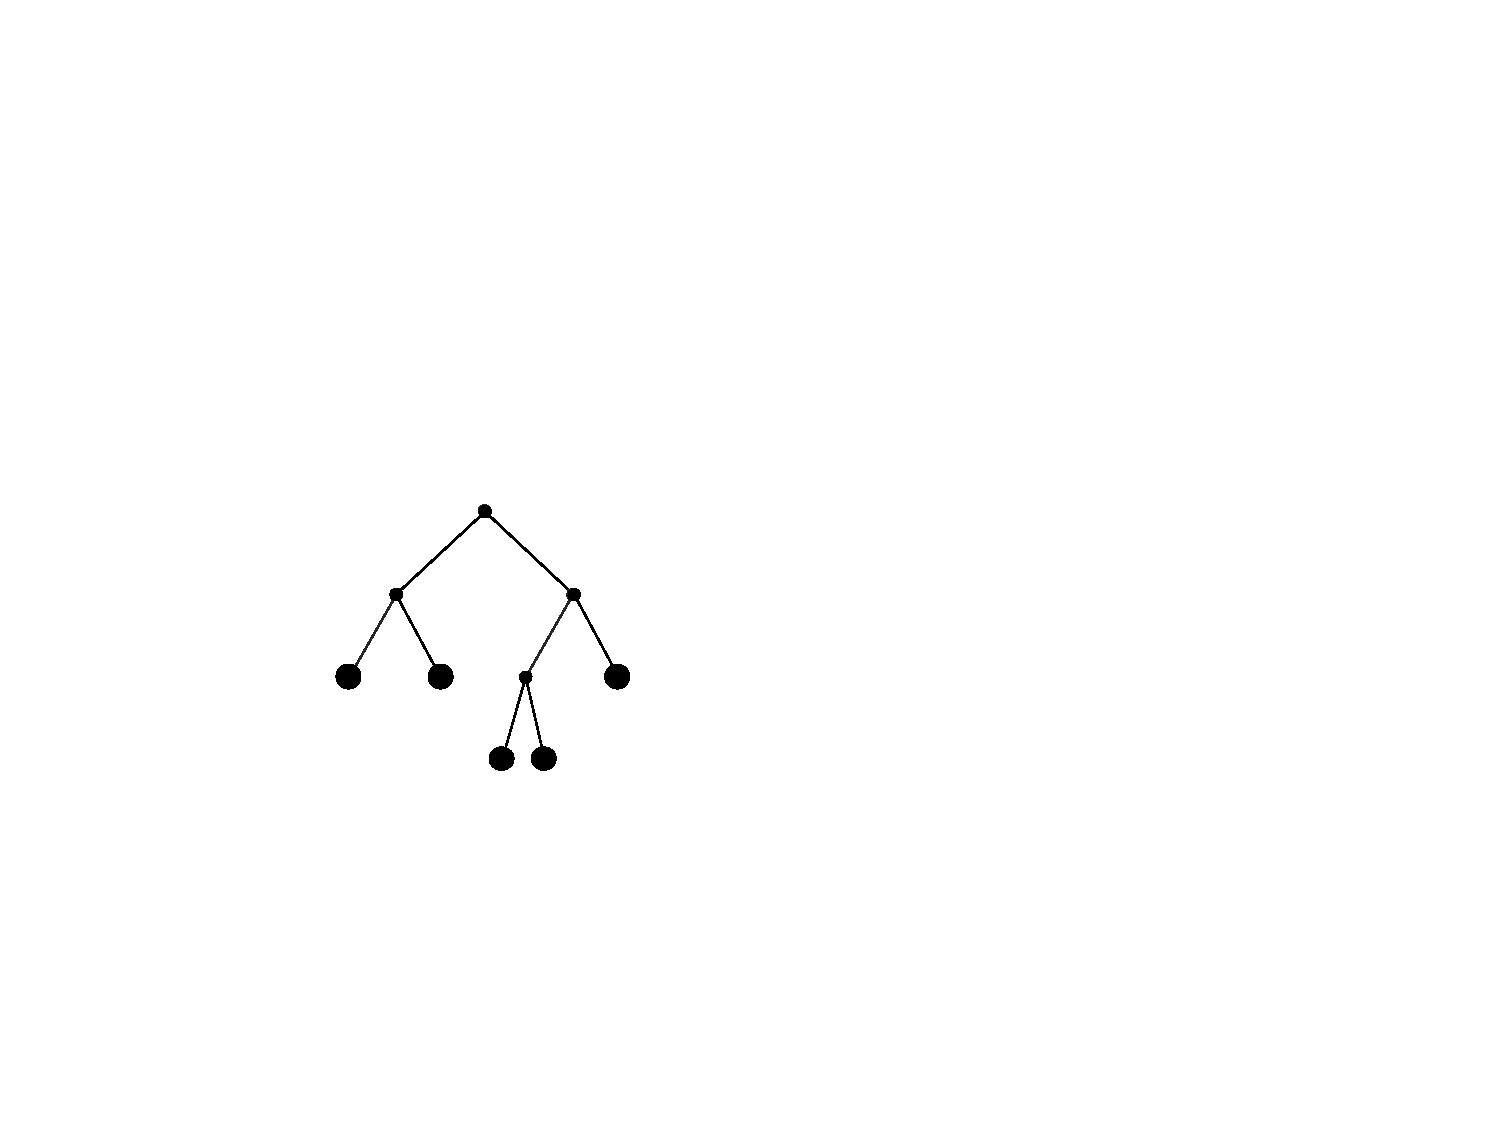
\includegraphics[width=\ratio\linewidth, trim={100 180 430 200}, clip]{schemas_strut_1_15.pdf}
        \onslide<7>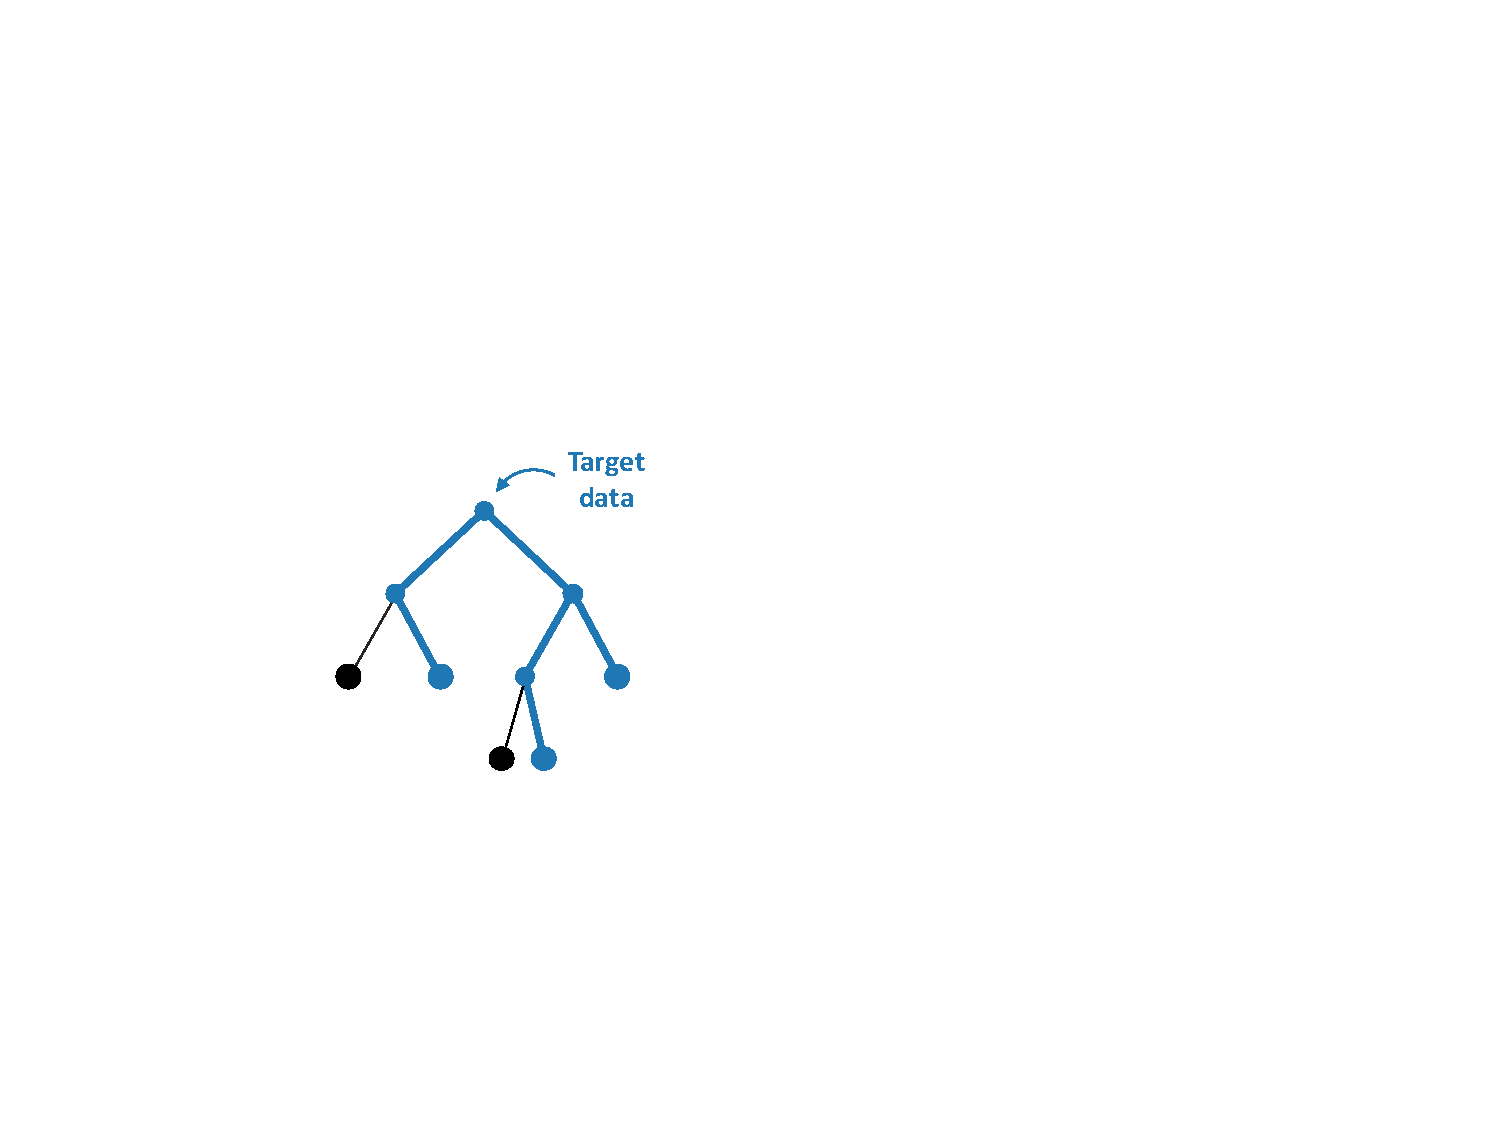
\includegraphics[width=\ratio\linewidth, trim={100 180 430 200}, clip]{schemas_strut_2_15.pdf}
        \onslide<8>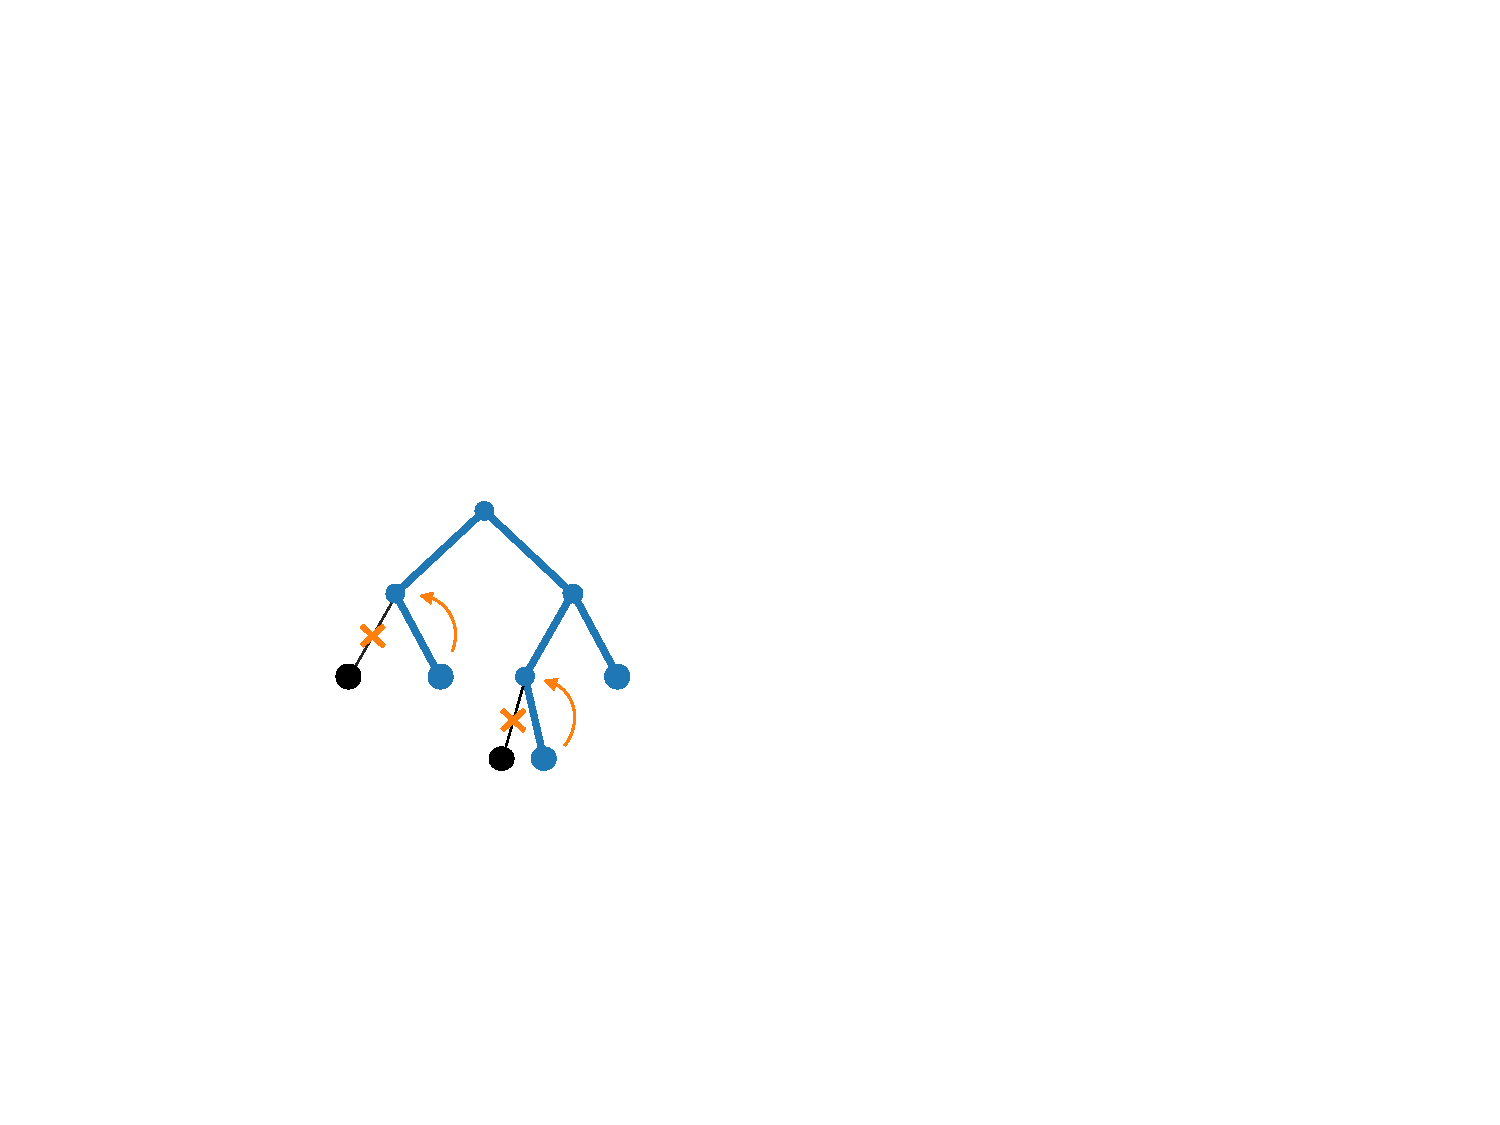
\includegraphics[width=\ratio\linewidth, trim={100 180 430 200}, clip]{schemas_strut_3_15.pdf}
        \onslide<9>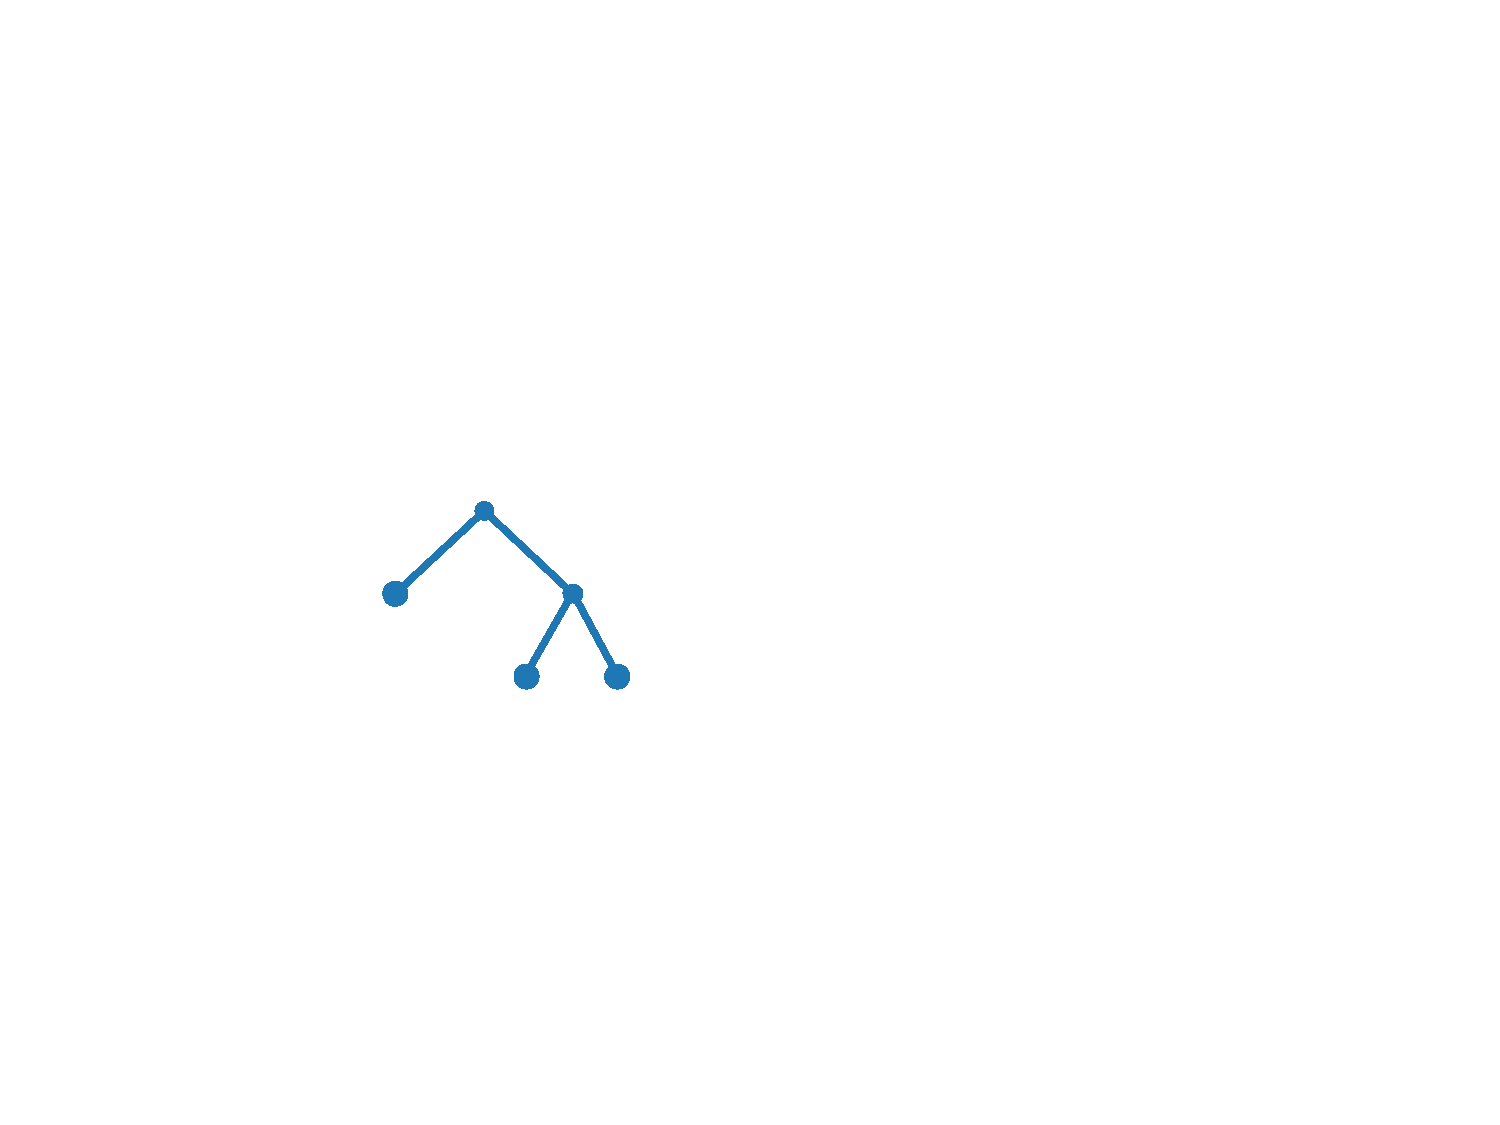
\includegraphics[width=\ratio\linewidth, trim={100 180 430 200}, clip]{schemas_strut_4_15.pdf}
        \onslide<10->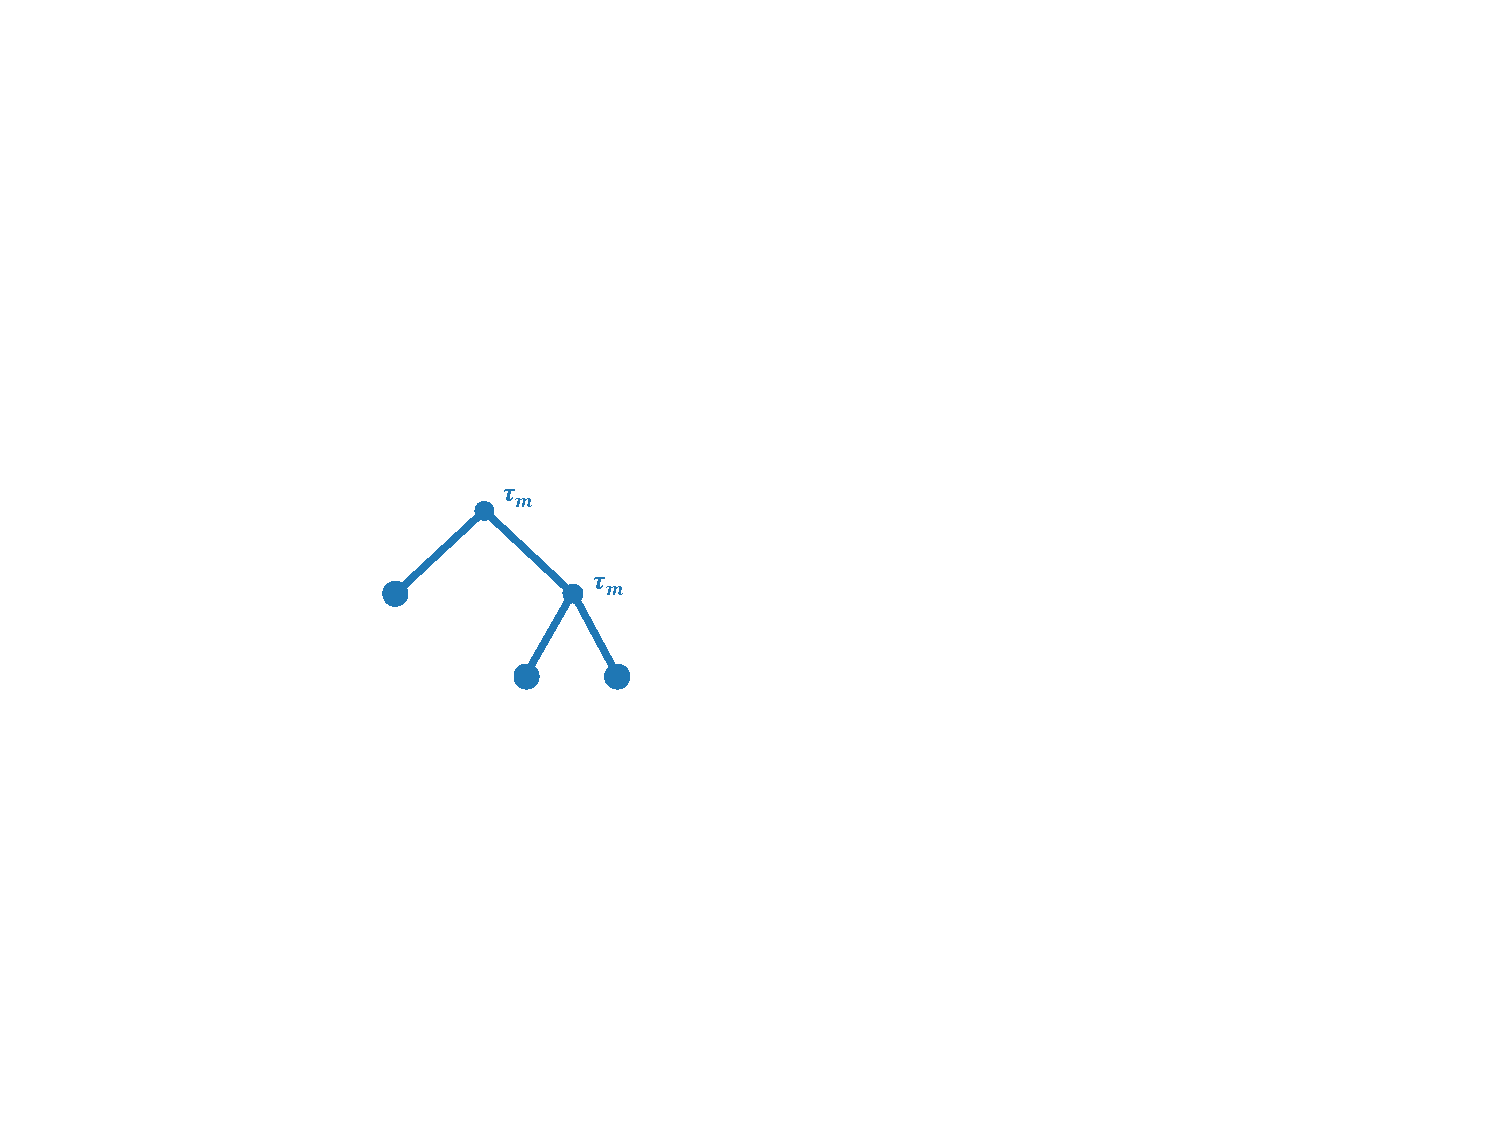
\includegraphics[width=\ratio\linewidth, trim={100 180 430 200}, clip]{schemas_strut_5_15.pdf}
    \end{overprint}

    \textcolor{myblue}{1. Pruning}\\
    \textcolor{myorange}{2. Threshold update}\\
    Drifts
\end{minipage}

\end{frame}

\begin{frame}{Transfer learning on decision tree}{Leaf loss risk}

\begin{minipage}[t]{0.38\textwidth}
    \vspace{0pt}
    \begin{tcolorbox}[title=Homogeneous class imbalance,size=title,boxrule=0.2pt]
    \begin{align*}
        & p^T(x/y) = p^S(x/y) \\
        & p^T(y/x) = \lambda_y \frac{p^S(y/x)}{\int{\lambda_y p^S(y/x)dy}}
    %       & \textrm{with} \quad \lambda_y = \frac{P_y^T}{P_y^S} 
    \end{align*}
        $\textrm{with} \quad \lambda_y = \frac{P_y^T}{P_y^S}$
    \end{tcolorbox}
\end{minipage}\hfill
\begin{minipage}[t]{0.59\textwidth}
    \vspace{0pt}
    \pause
    \begin{tcolorbox}[title=Leaf loss risk,size=title,boxrule=0.2pt]
            Leaf $l$ that conserves the minority class $k_{min}$ after Target update
        \begin{equation*}
        \forall k \neq k_{min},\quad {p}^T(y = k_{min} / x \in l) > {p}^T(y = k / x \in l) 
        \label{eqF_rep_targ}
        \end{equation*}
        Risk of losing the leaf:
        \begin{equation*}
        R_{n_{k_{min}}}(l)={p}^T(x \notin l / y = k_{min})^{n_{k_{min}}} 
        \label{eq_risk_value}
        \end{equation*}
        \pause
        In homogeneous class imbalance:
        \begin{equation*}
        \forall k \neq k_{min}, \quad \lambda_{k_{min}}  {p}^S(y = k_{min} / x \in l) > \lambda_k  {p}^S(y = k / x \in l)
        \end{equation*}
        \begin{equation*}
        R_{n_{k_{min}}}(l)={p}^S(x \notin l / y = k_{min})^{n_{k_{min}}}
        \end{equation*}
    \end{tcolorbox}
\end{minipage}

\end{frame}

\begin{frame}{Transfer learning on decision tree}{Leaf loss risk}
\renewcommand{\ratio}{0.78}
\renewcommand{\ratiob}{0.45}
    \centering
    \begin{minipage}[t]{0.8\linewidth}\vspace{0pt}
        \centering
        \begin{minipage}[t]{\ratiob\linewidth}\vspace{0pt}
            \centering
            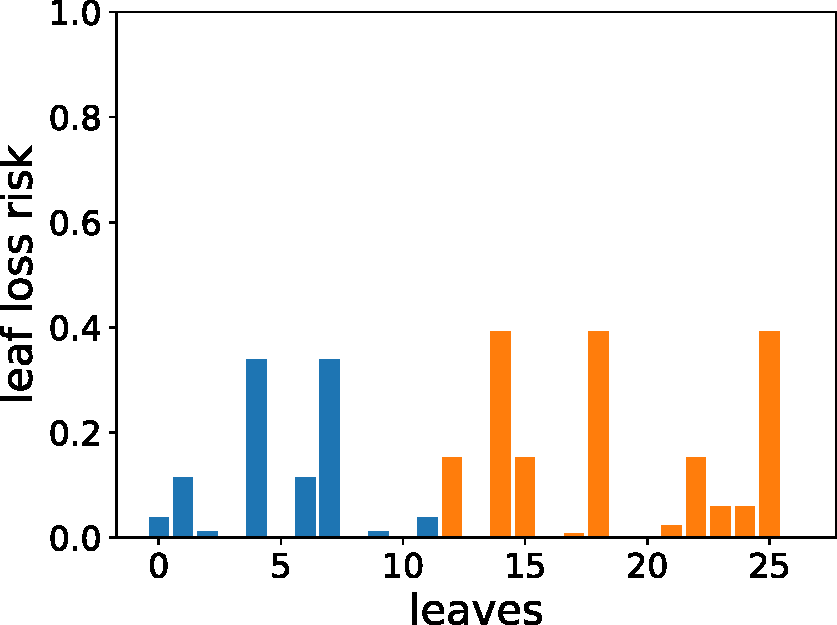
\includegraphics[width=\ratio\linewidth]{leaf_loss_NTarget200_Lambda1.pdf}\\
            {\small(a)\; Balanced data with 200 instances}
        \end{minipage}\vspace{0.2cm}
        \begin{minipage}[t]{\ratiob\linewidth}\vspace{0pt}
            \centering
            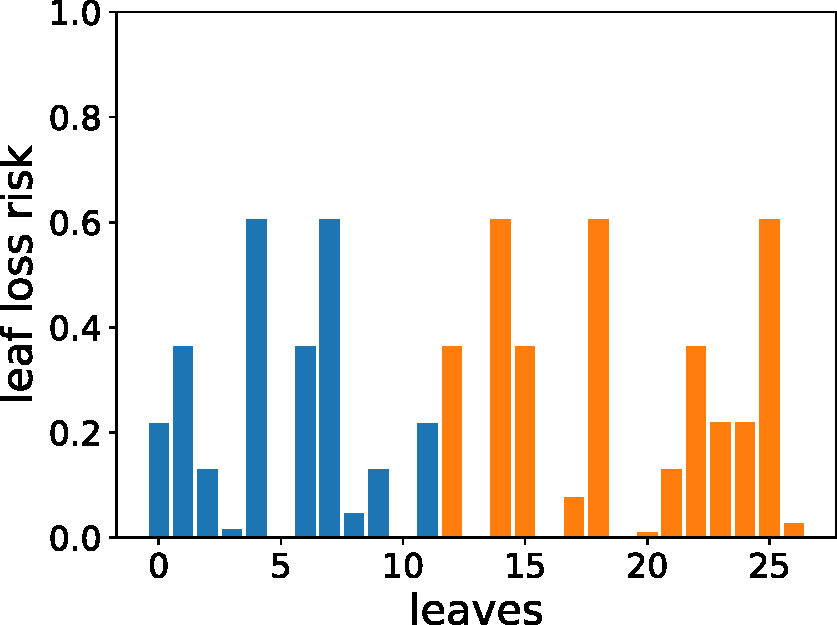
\includegraphics[width=\ratio\linewidth]{leaf_loss_NTarget100_Lambda1.pdf}\\
            {\small(b)\; Balanced data with 100 instances }
        \end{minipage}
        % \hfill
        \\
        \begin{minipage}[t]{\ratiob\linewidth}\vspace{0pt}
            \centering
            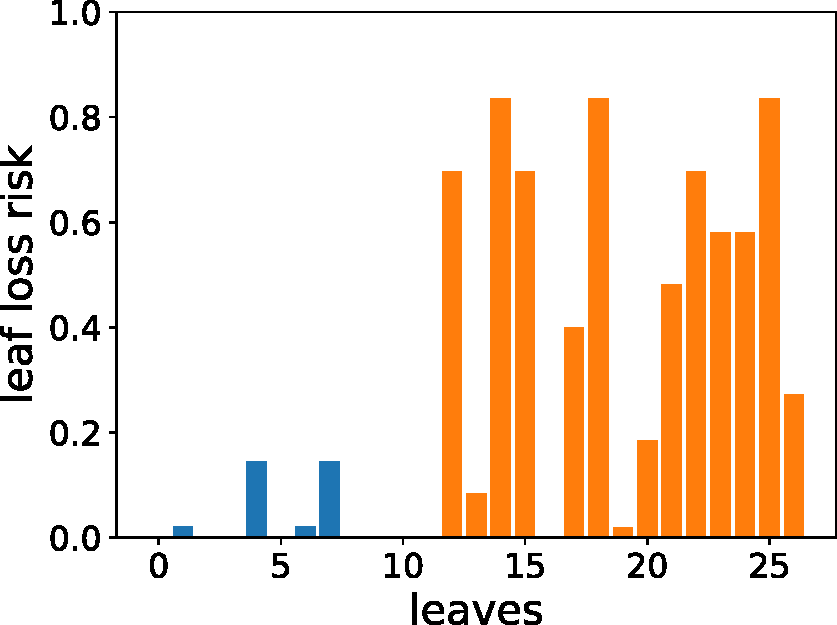
\includegraphics[width=\ratio\linewidth]{leaf_loss_NTarget200_Lambda01.pdf}\\
            {\small (c)\; Imbalanced data (10\% ratio) with 200 instances}
        \end{minipage}
        \centering
        \begin{minipage}[t]{\ratiob\linewidth}\vspace{0pt}
            \centering
            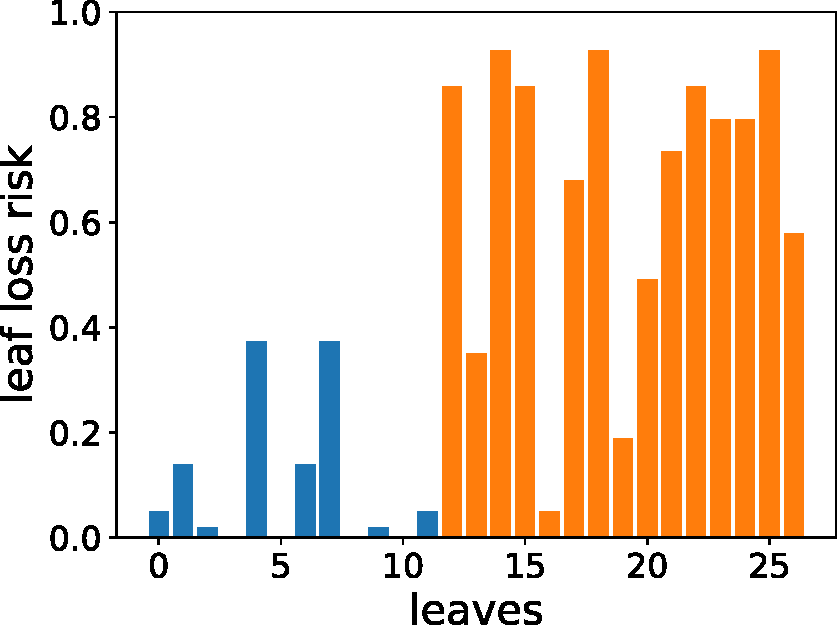
\includegraphics[width=\ratio\linewidth]{leaf_loss_NTarget100_Lambda01.pdf}\\
            {\small (d)\; Imbalanced data (10\% ratio) with 100 instances}
        \end{minipage}\vspace{0.1cm}
    \end{minipage}

\end{frame}

\begin{frame}{Transfer learning on decision tree}{SER for class imbalance}
\begin{minipage}[t]{0.49\linewidth}
    \vspace{0pt}
    
    \centering
    \textbf{Structure Expansion/Reduction}\\
        
    \renewcommand{\ratio}{0.8}
    \begin{overprint}
        \onslide<1>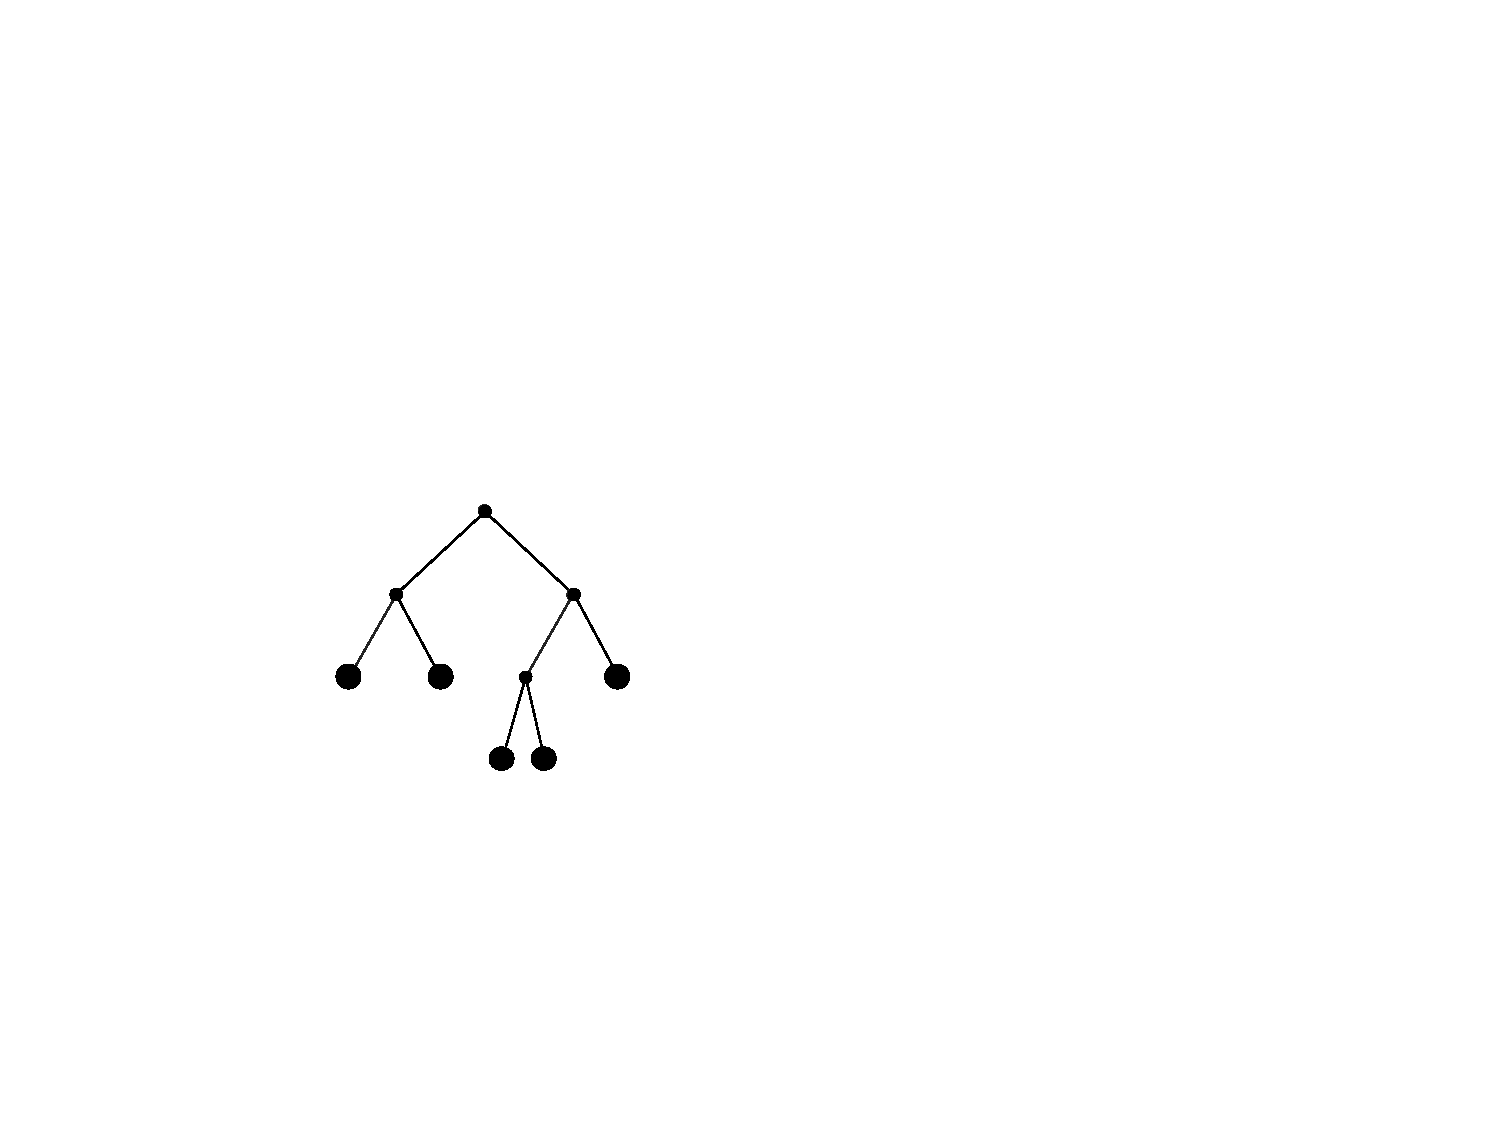
\includegraphics[width=\ratio\linewidth, trim={100 120 390 200}, clip]{schemas_ser_1.pdf}
        \onslide<2>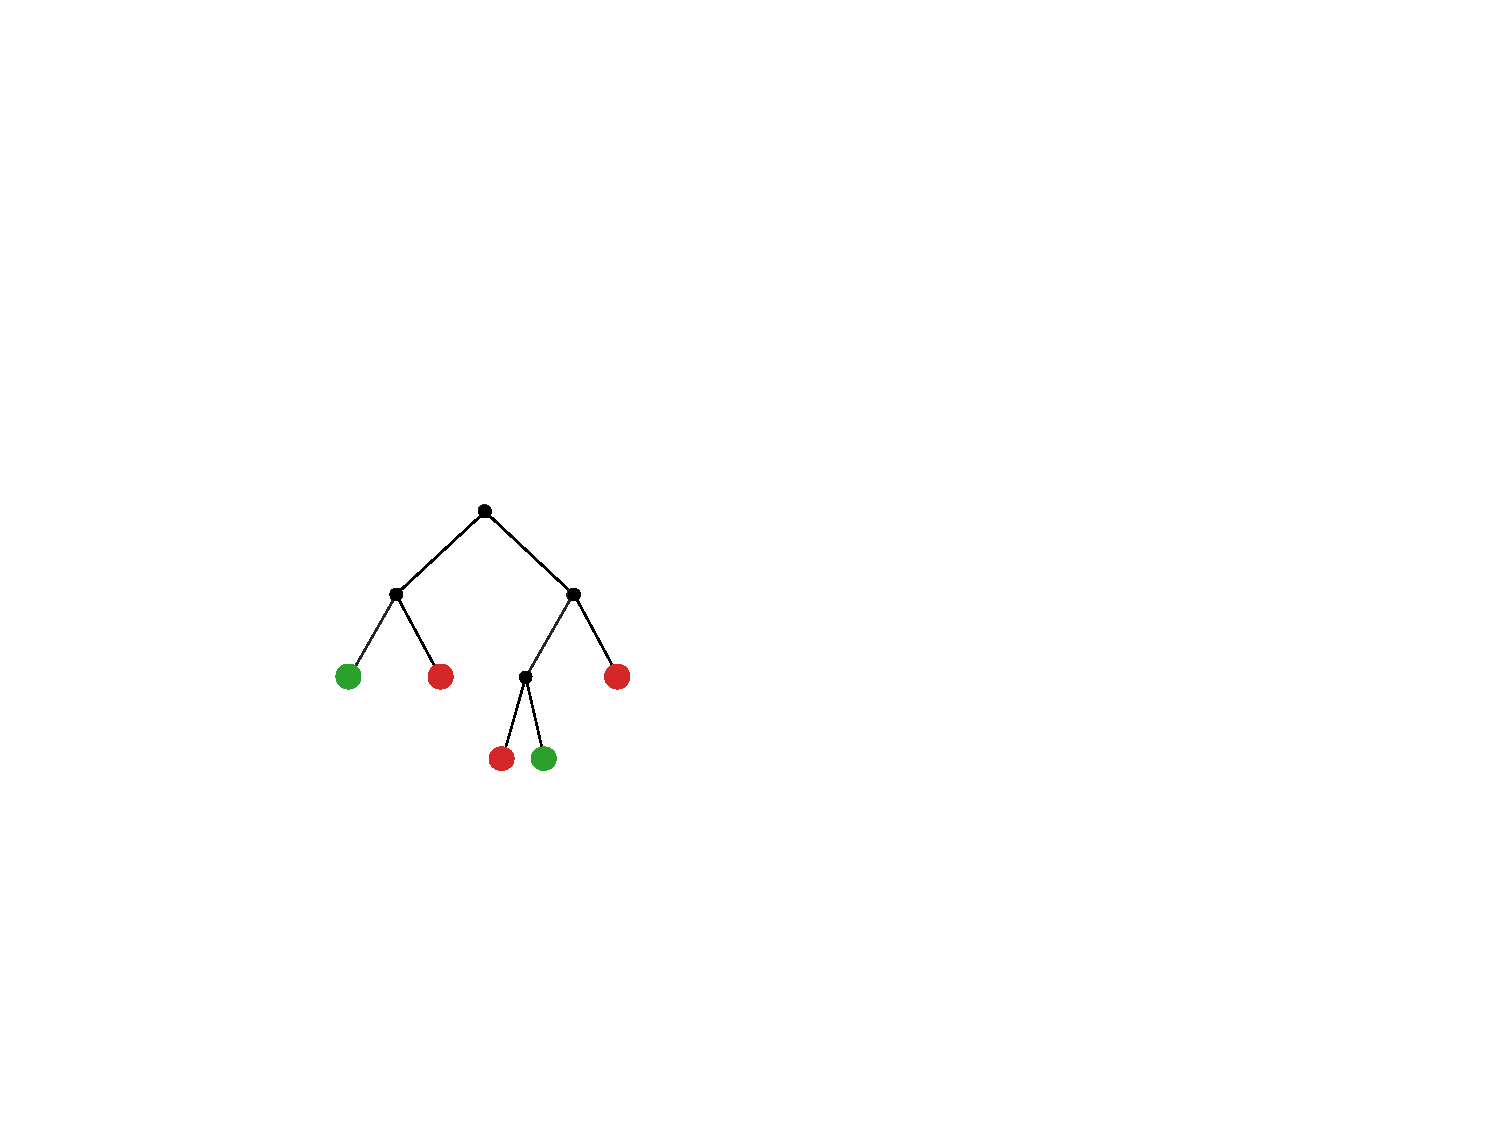
\includegraphics[width=\ratio\linewidth, trim={100 120 390 200}, clip]{schemas_sernr_1_15.pdf}
        \onslide<3>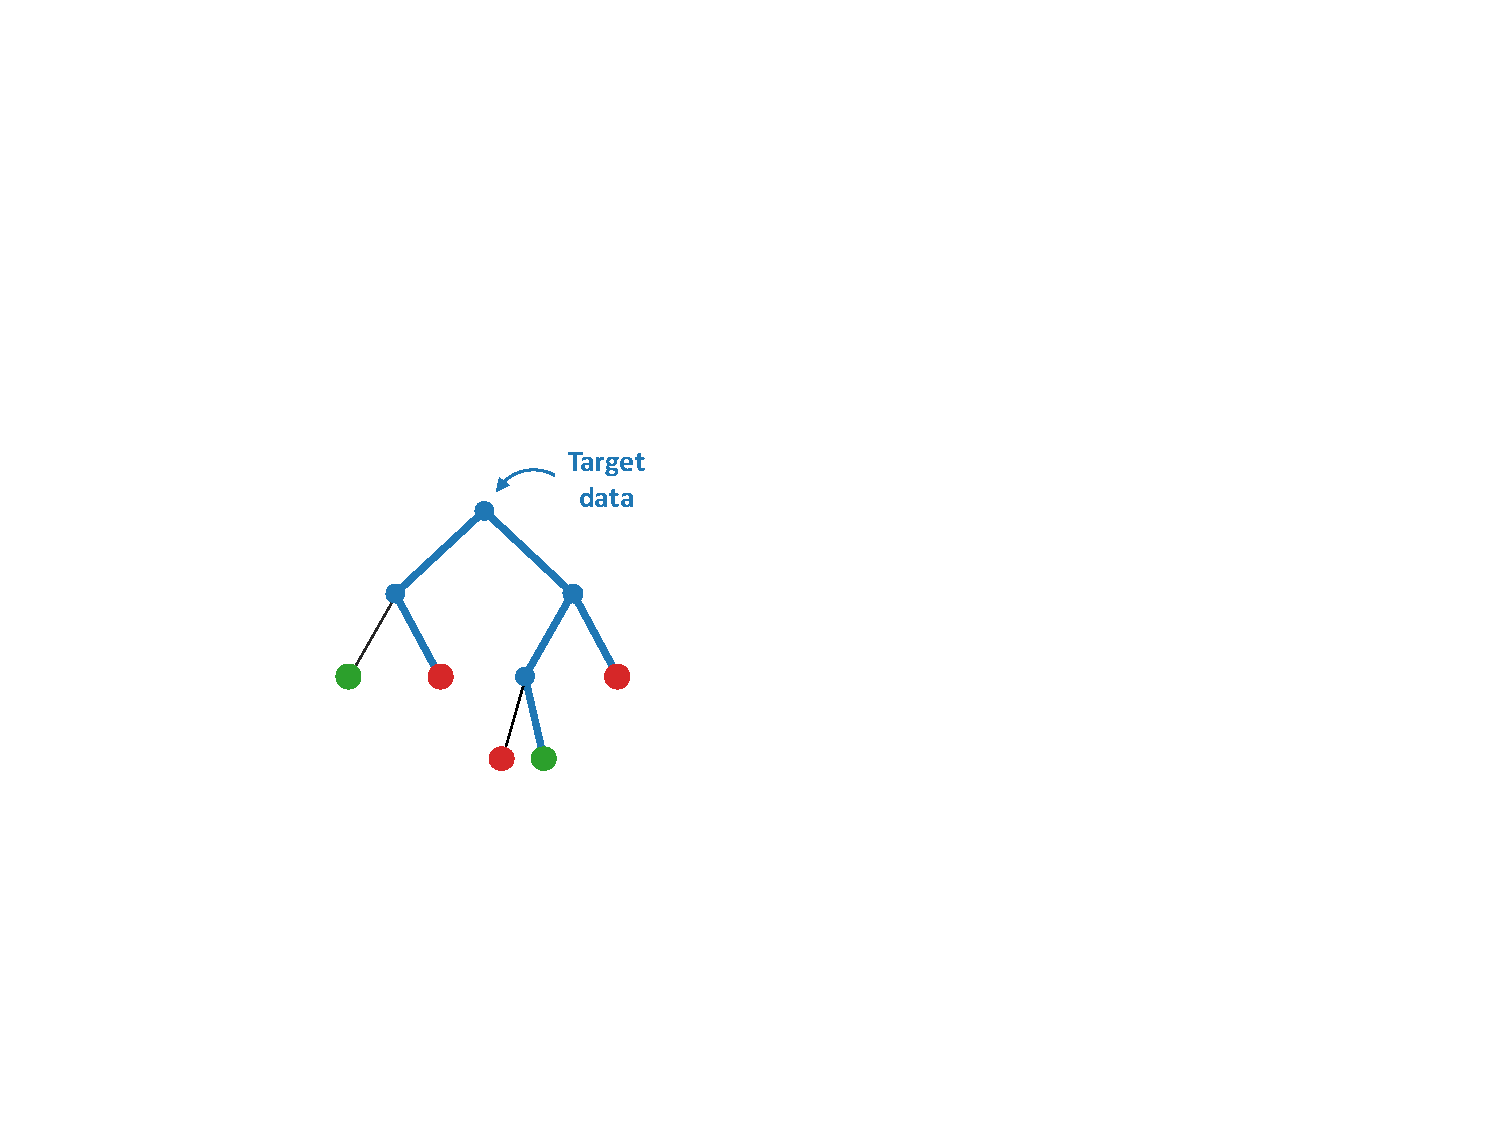
\includegraphics[width=\ratio\linewidth, trim={100 120 390 200}, clip]{schemas_sernr_2_15.pdf}
        \onslide<4>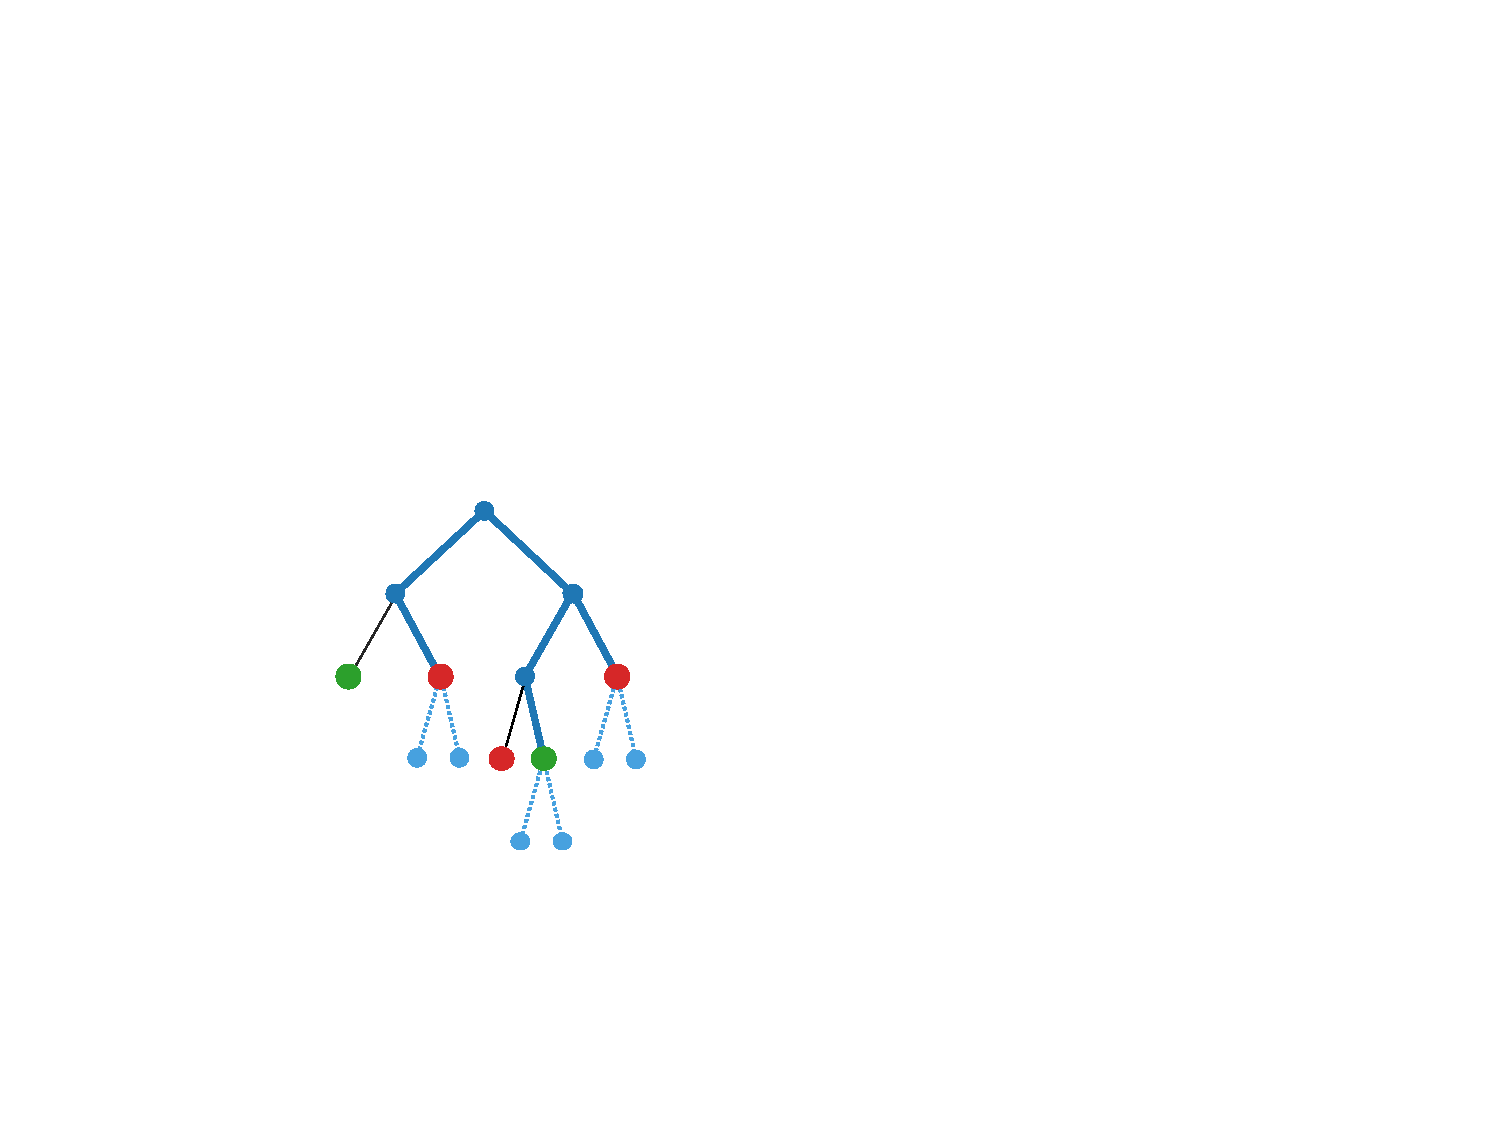
\includegraphics[width=\ratio\linewidth, trim={100 120 390 200}, clip]{schemas_sernr_3_15.pdf}
        \onslide<5>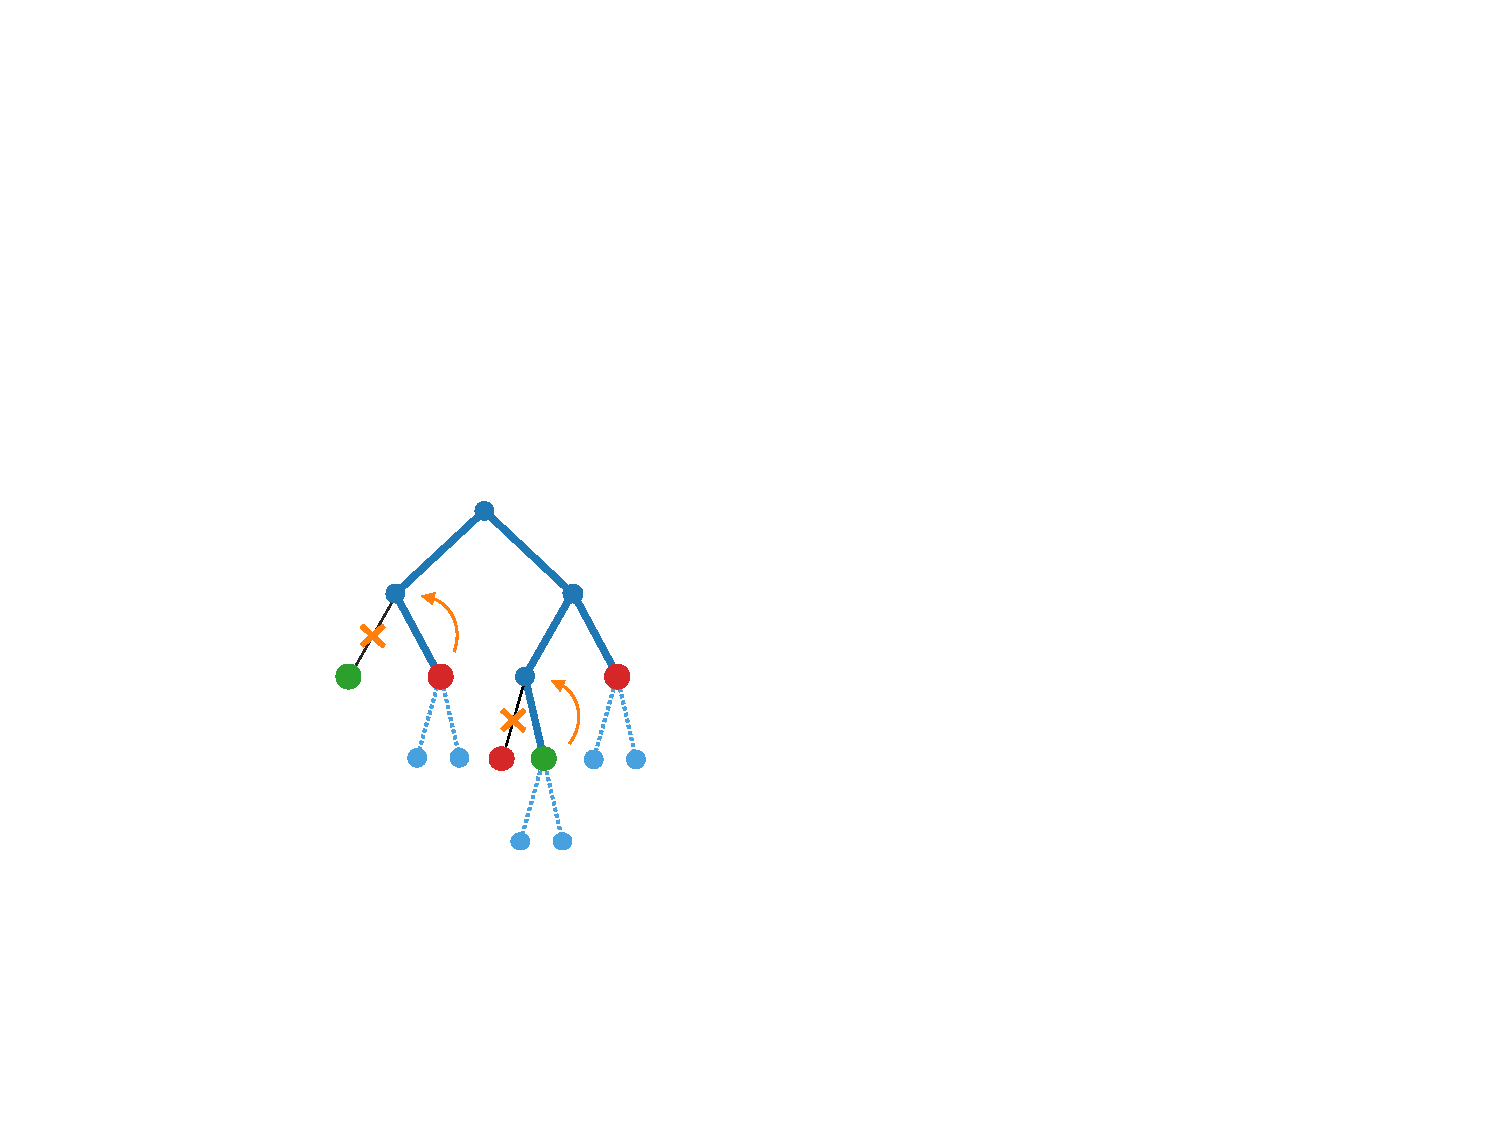
\includegraphics[width=\ratio\linewidth, trim={100 120 390 200}, clip]{schemas_sernr_4_15.pdf}
        \onslide<6>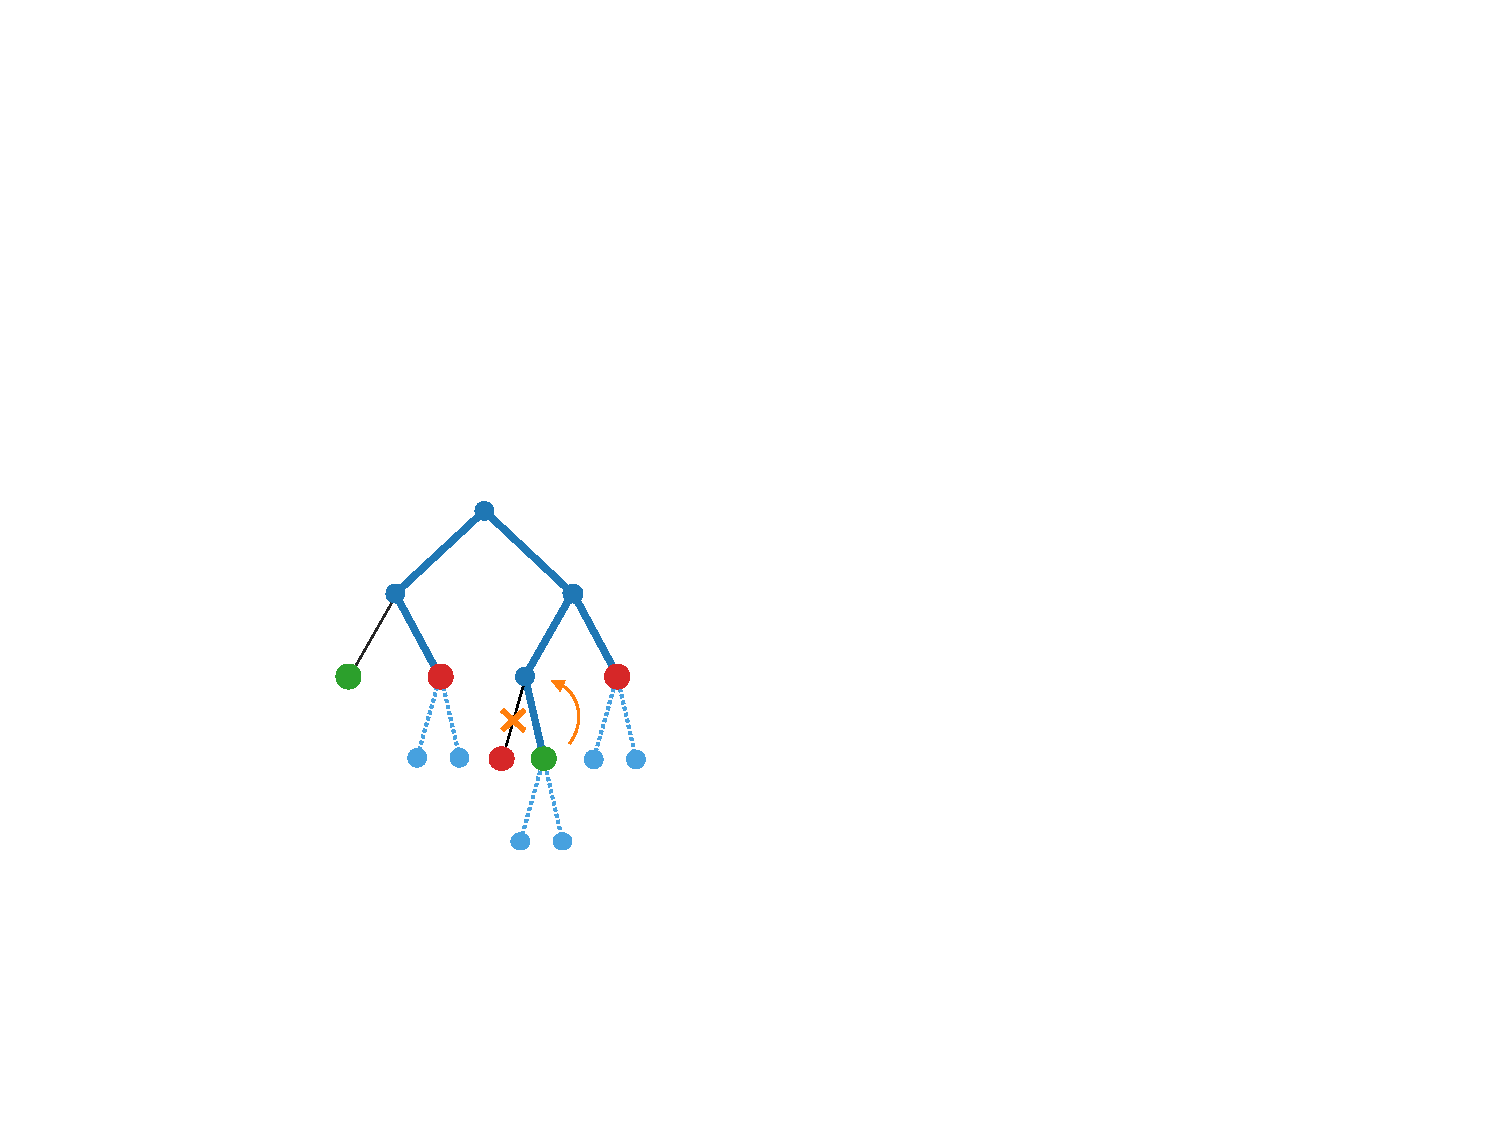
\includegraphics[width=\ratio\linewidth, trim={100 120 390 200}, clip]{schemas_sernr_5_15.pdf}
        \onslide<7->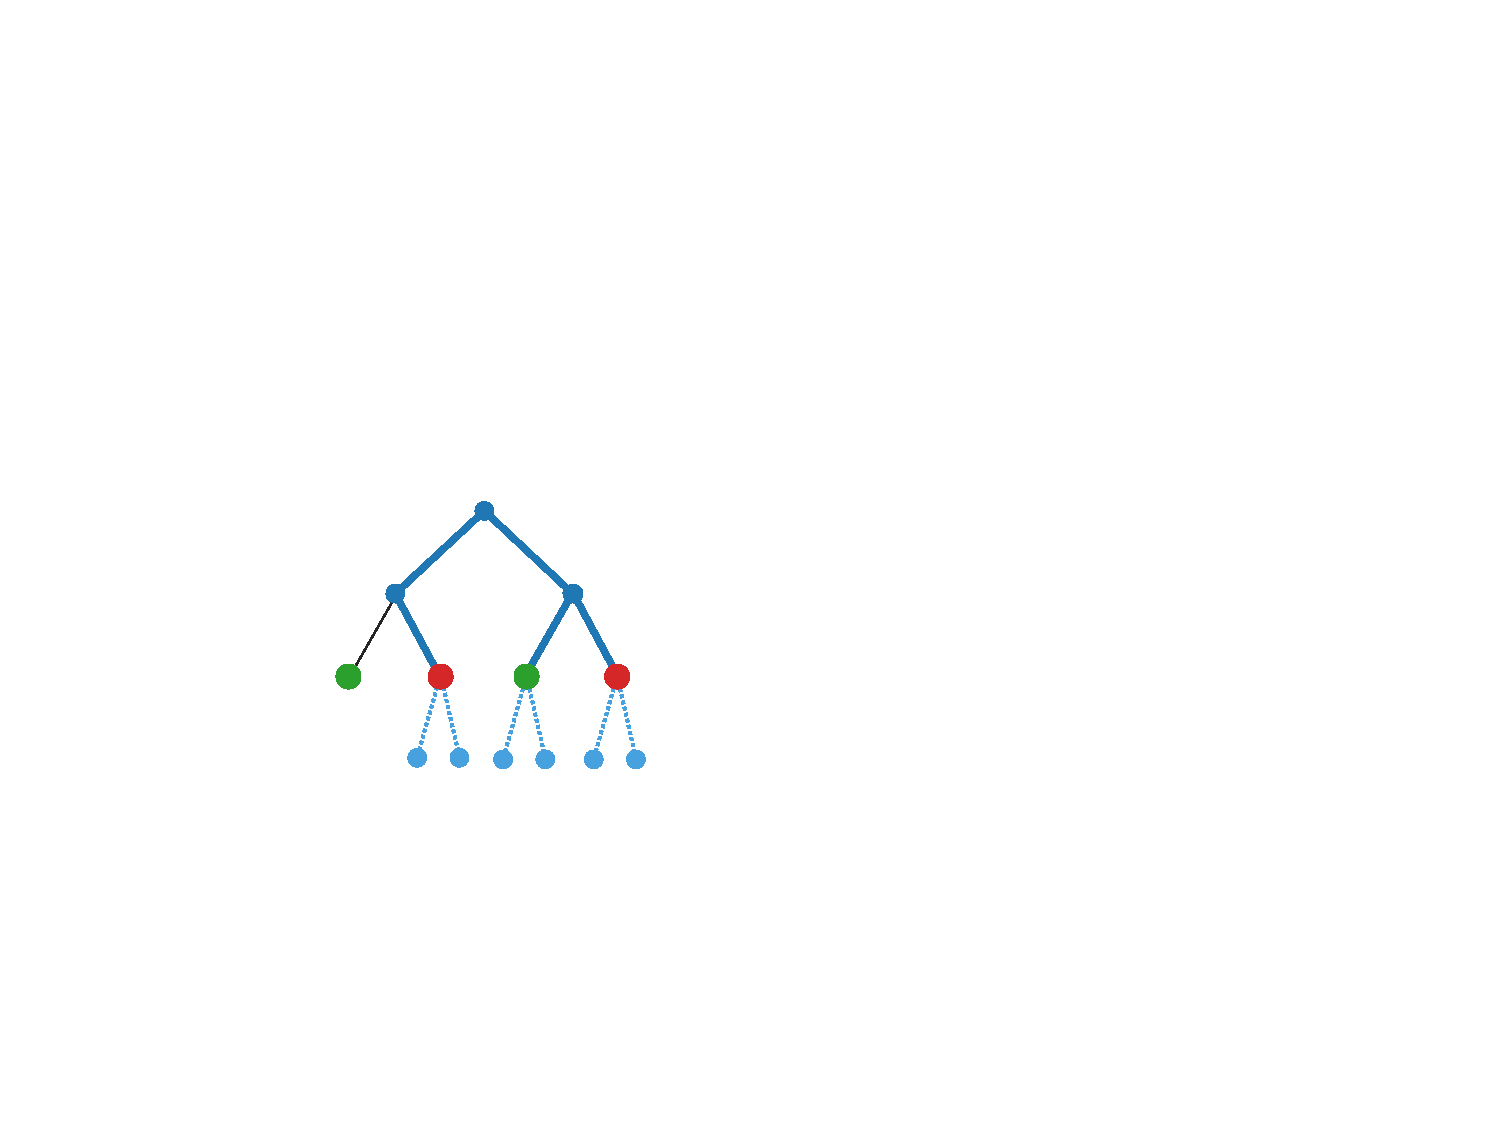
\includegraphics[width=\ratio\linewidth, trim={100 120 390 200}, clip]{schemas_sernr_6_15.pdf}
    \end{overprint}
    \textcolor{mygreen}{\textbf{Minority class}}
\end{minipage}\hfill
\begin{minipage}[t]{0.35\linewidth}
    \vspace{0pt}
    \vspace{1.5cm}
    \begin{itemize}
    \item Extension left unchanged
    \item Reduction constrained
    \end{itemize}
%     \begin{tcolorbox}
%         
%     \end{tcolorbox}

    

\end{minipage}

\end{frame}

\begin{frame}{Transfer learning on decision tree}{STRUT optimization}

\begin{minipage}[t]{0.4\linewidth}
    \vspace{0pt}
    
    \centering
    \textbf{STRUT}\\

    \renewcommand{\ratio}{1.0}
    \begin{overprint}
        \onslide<1>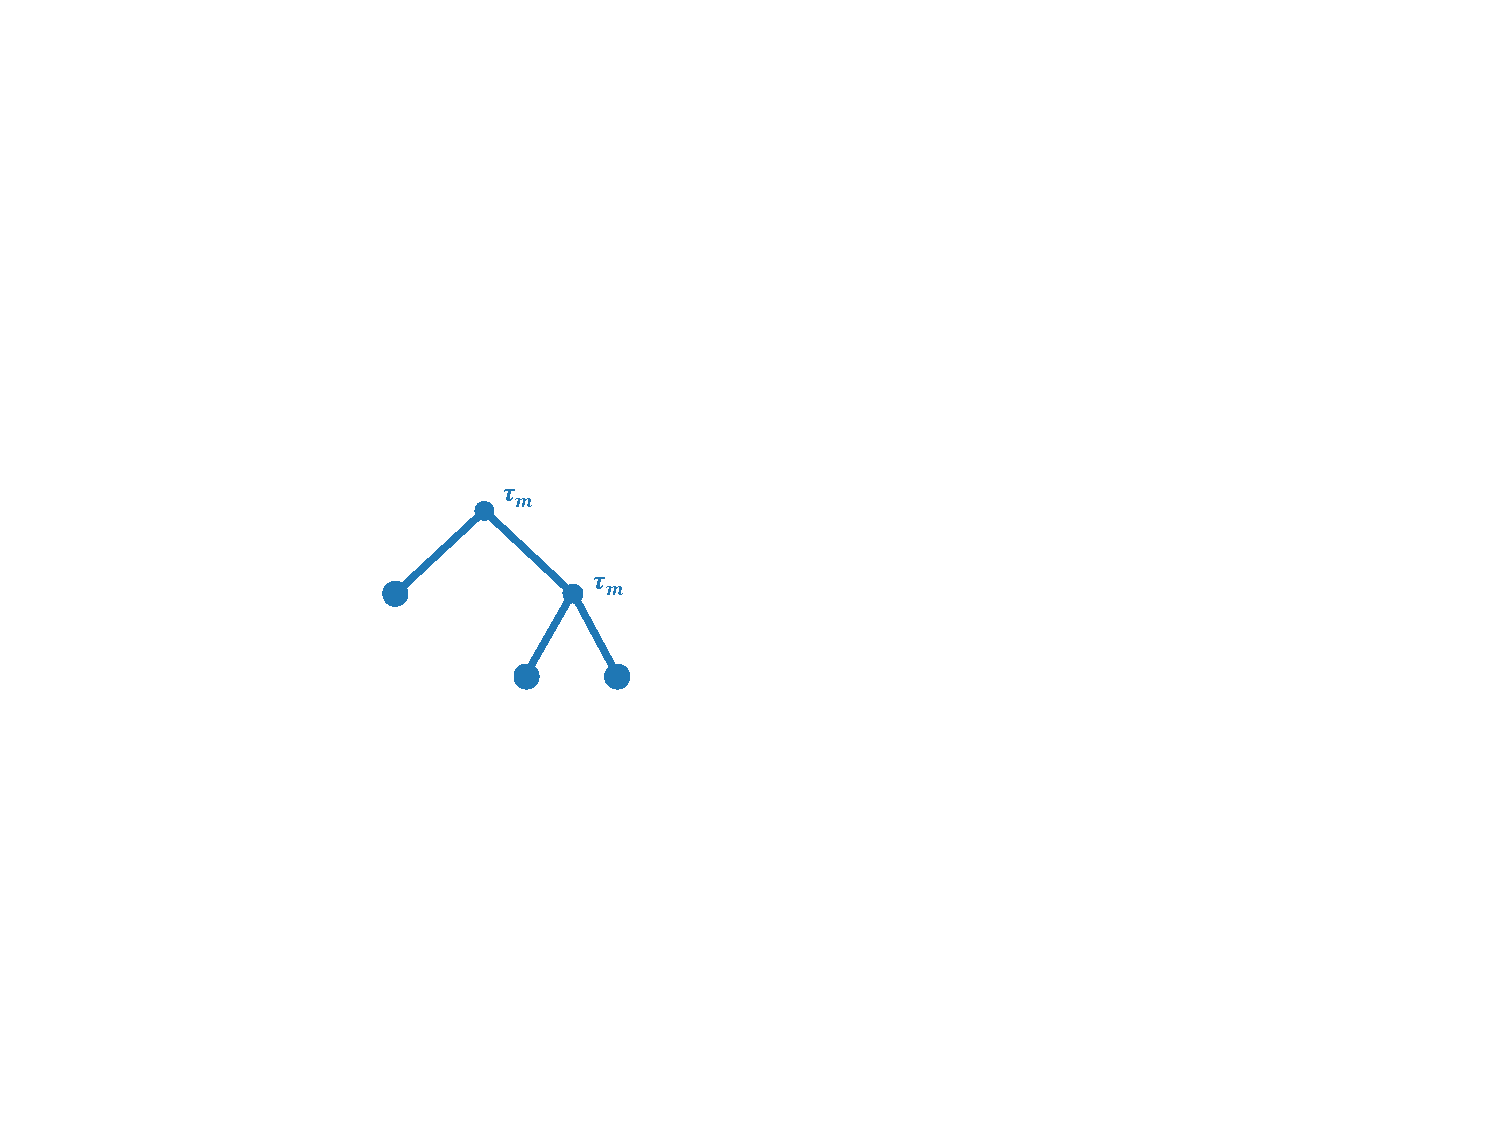
\includegraphics[width=\ratio\linewidth, trim={150 120 320 200}, clip]{schemas_strutoptim_0_15.pdf}
        \onslide<2>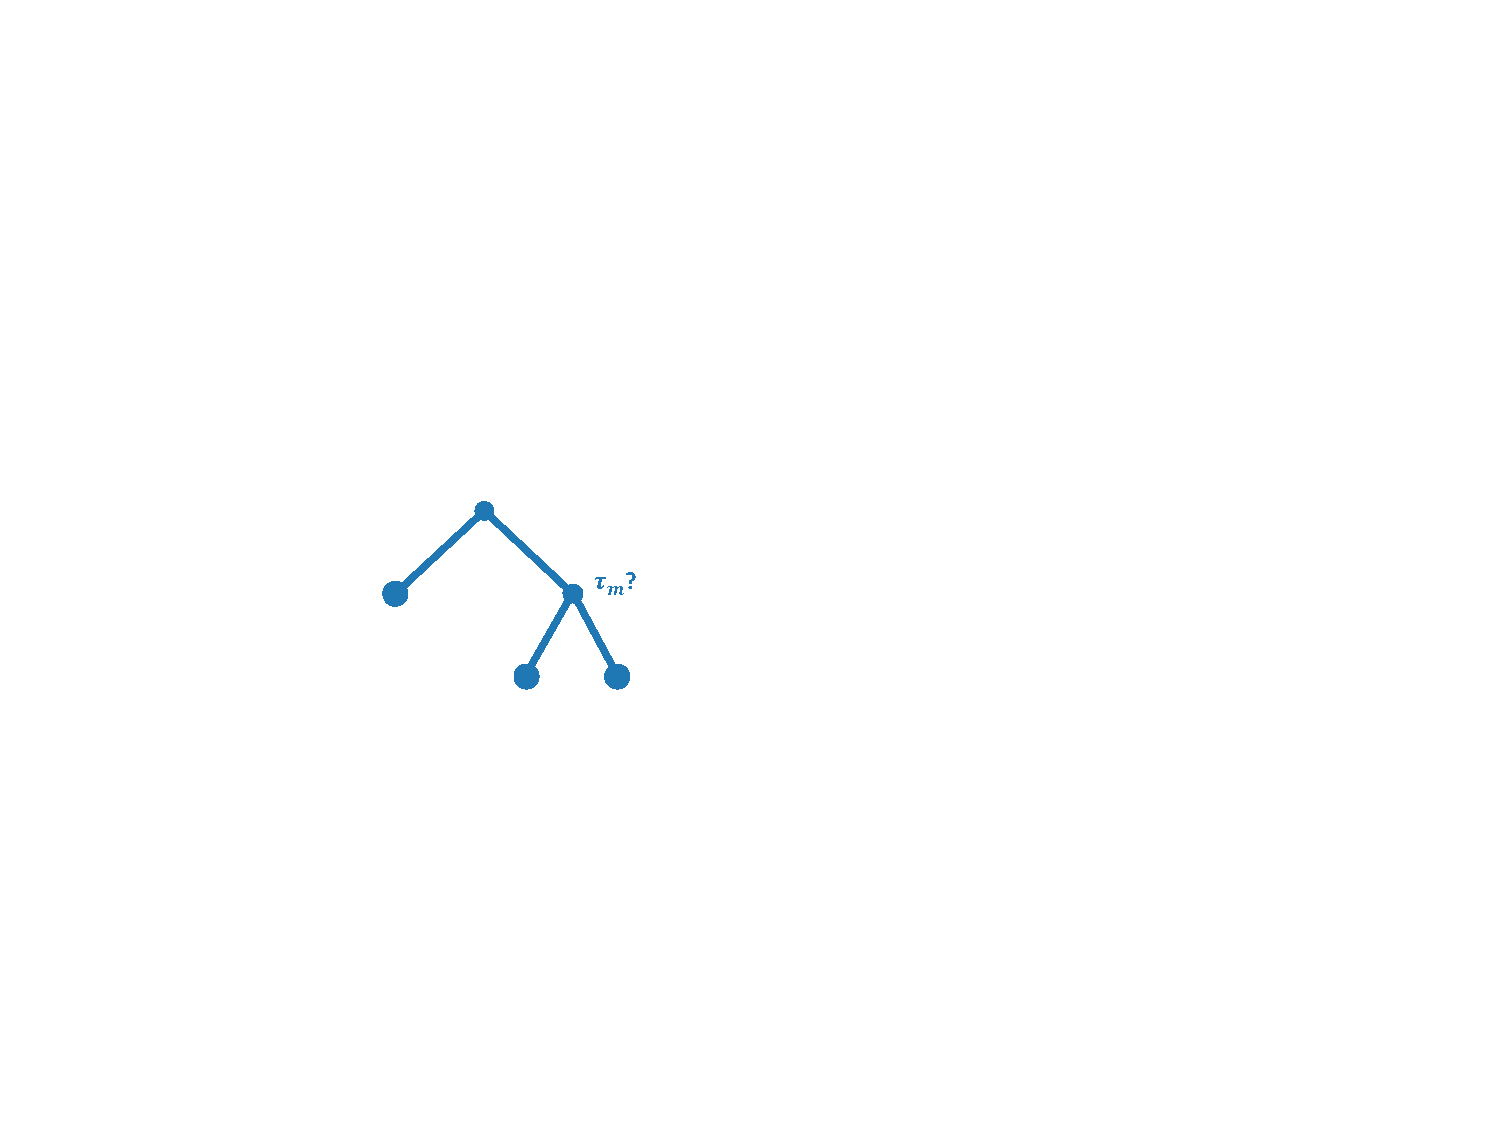
\includegraphics[width=\ratio\linewidth, trim={150 120 320 200}, clip]{schemas_strutoptim_1_15.pdf}
        \onslide<3>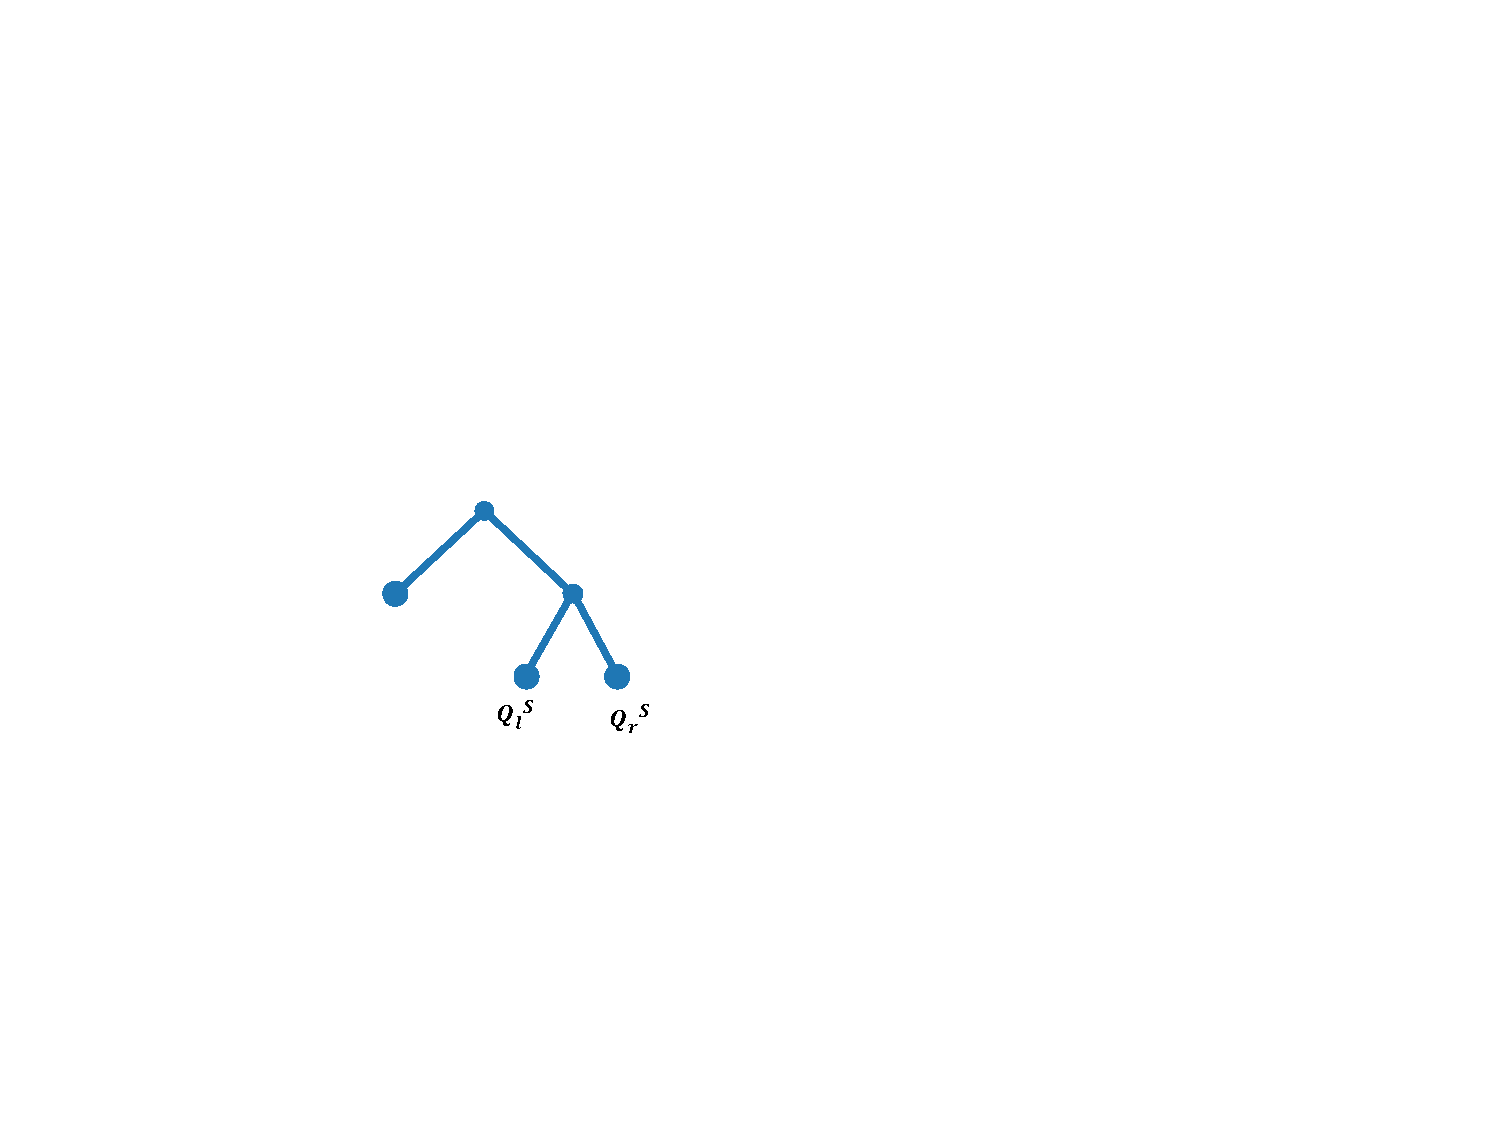
\includegraphics[width=\ratio\linewidth, trim={150 120 320 200}, clip]{schemas_strutoptim_2_15.pdf}
    \end{overprint}
\end{minipage}\hfill
\begin{minipage}[t]{0.55\linewidth}
    \vspace{0pt}
    \pause \pause
    $Q_{l}^{S}$, $Q_{r}^{S}$: class proportions of source data in children w.r.t.\ the \emph{original} split\\
    \pause
    $S_{v,l}^{T}$, $S_{v,r}^{T}$: subsets of $S_{v}^{T}$ that fall in the children nodes of $v$\\
    $Q_{l}^{T}(\tau)$, $Q_{r}^{T}(\tau)$: class proportions of target data in children w.r.t.\ the \emph{new} split\\
    \pause
    \textbf{Divergence Gain}: similarity between the original label distributions and the new ones
    $$
    DG\left(\tau\right) = 1 - \frac{|S_{v,l}^{T}|}{|S_{v}^{T}|}JSD(Q_{l}^{S}, Q_{l}^{T})
    - \frac{|S_{v,r}^{T}|}{|S_{v}^{T}|}JSD(Q_{r}^{S}, Q_{r}^{T})
    $$
%     \footnotesize
    Jensen-Shannon divergence:
    $$JSD(P, Q) = \frac{1}{2}\left(D_{KL}(P||M) + D_{KL}(Q||M)\right) $$
    \begin{flushright}
    $M = \frac{1}{2} \left(P +Q\right) $
    \end{flushright}
    Kullback-Leibler divergence:
    $$D_{KL}(P||Q) = \sum_{k}{P(k)\ln\left(\frac{P(k)}{Q(k)}\right)}$$


\end{minipage}

\end{frame}

\begin{frame}{Transfer learning on decision tree}{STRUT optimization}
\begin{minipage}[t]{0.4\linewidth}
    \vspace{0pt}
    \renewcommand{\ratio}{1.0}
    \begin{overprint}
        \onslide<1>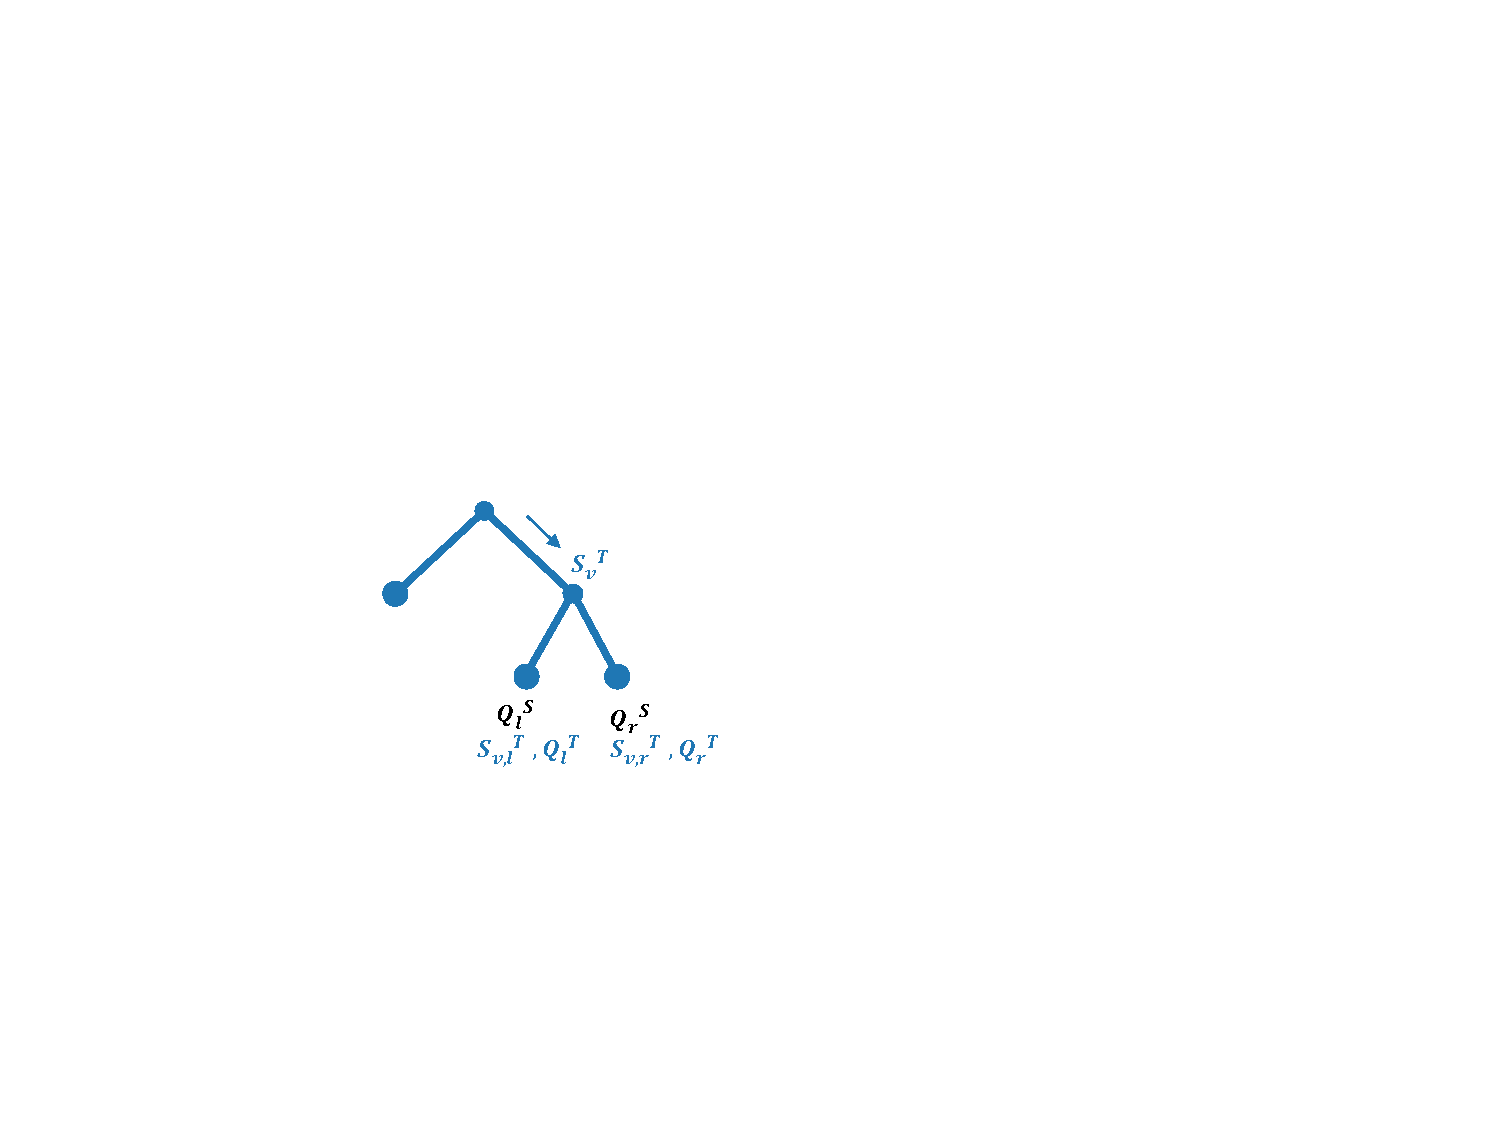
\includegraphics[width=\ratio\linewidth, trim={150 120 320 200}, clip]{schemas_strutoptim_3_15.pdf}
        \onslide<2>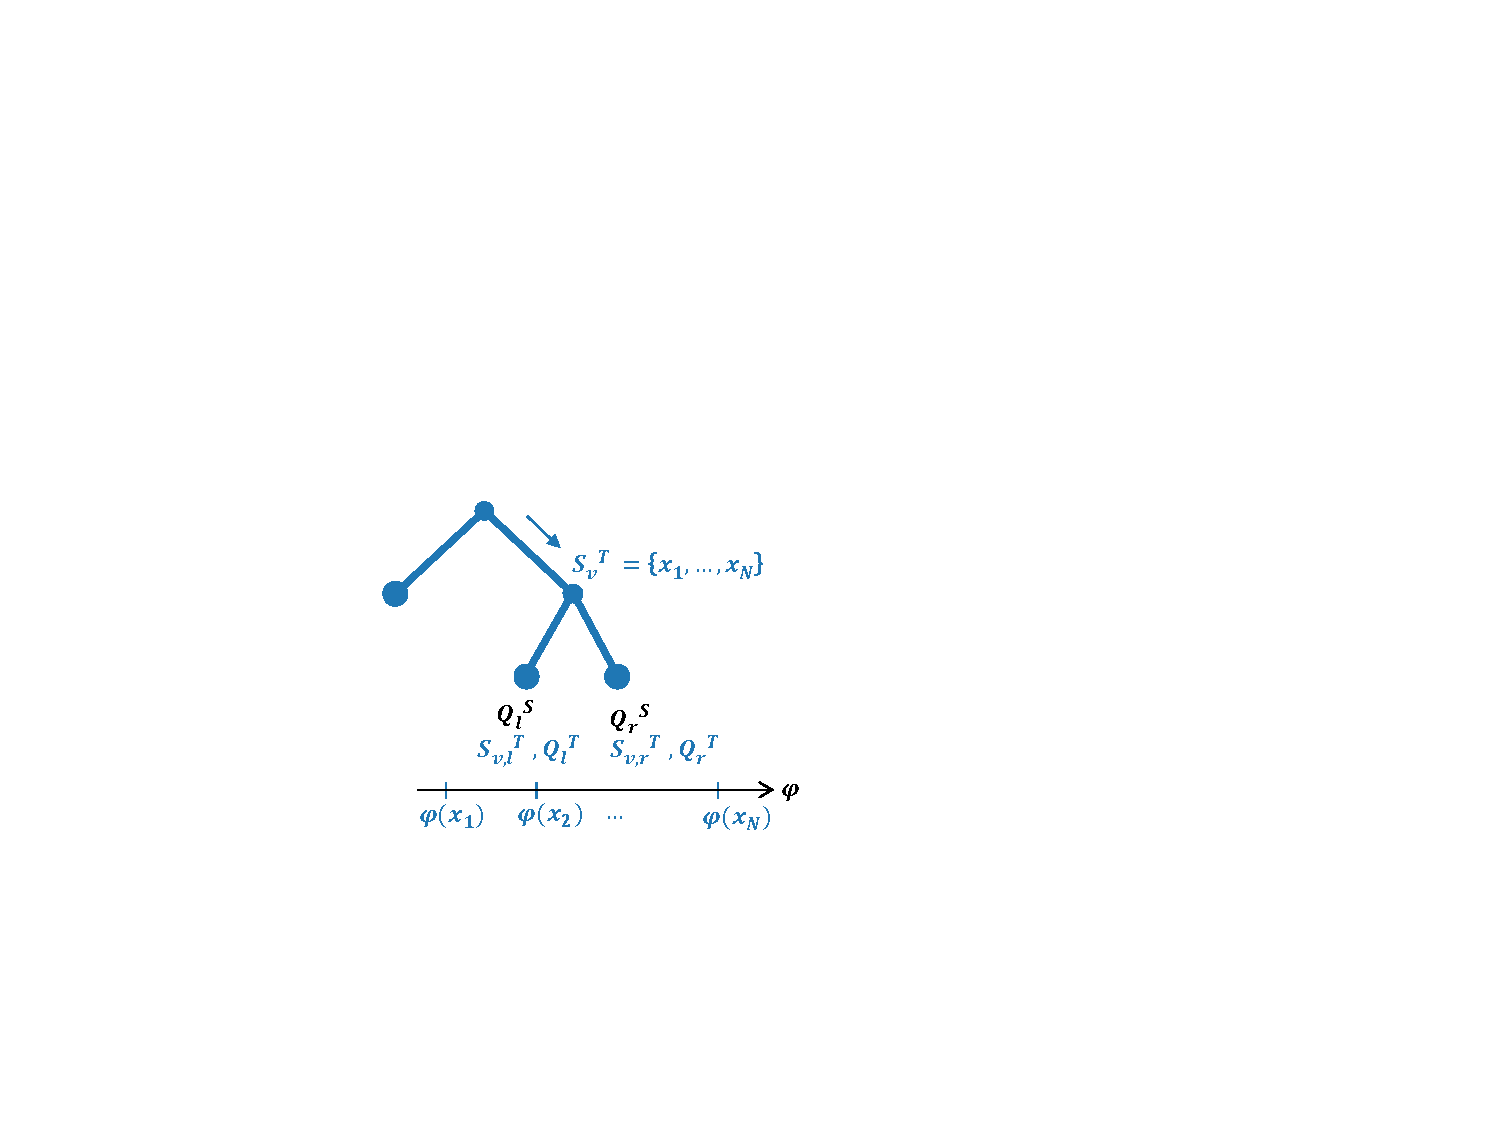
\includegraphics[width=\ratio\linewidth, trim={150 120 320 200}, clip]{schemas_strutoptim_4_15.pdf}
        \onslide<3->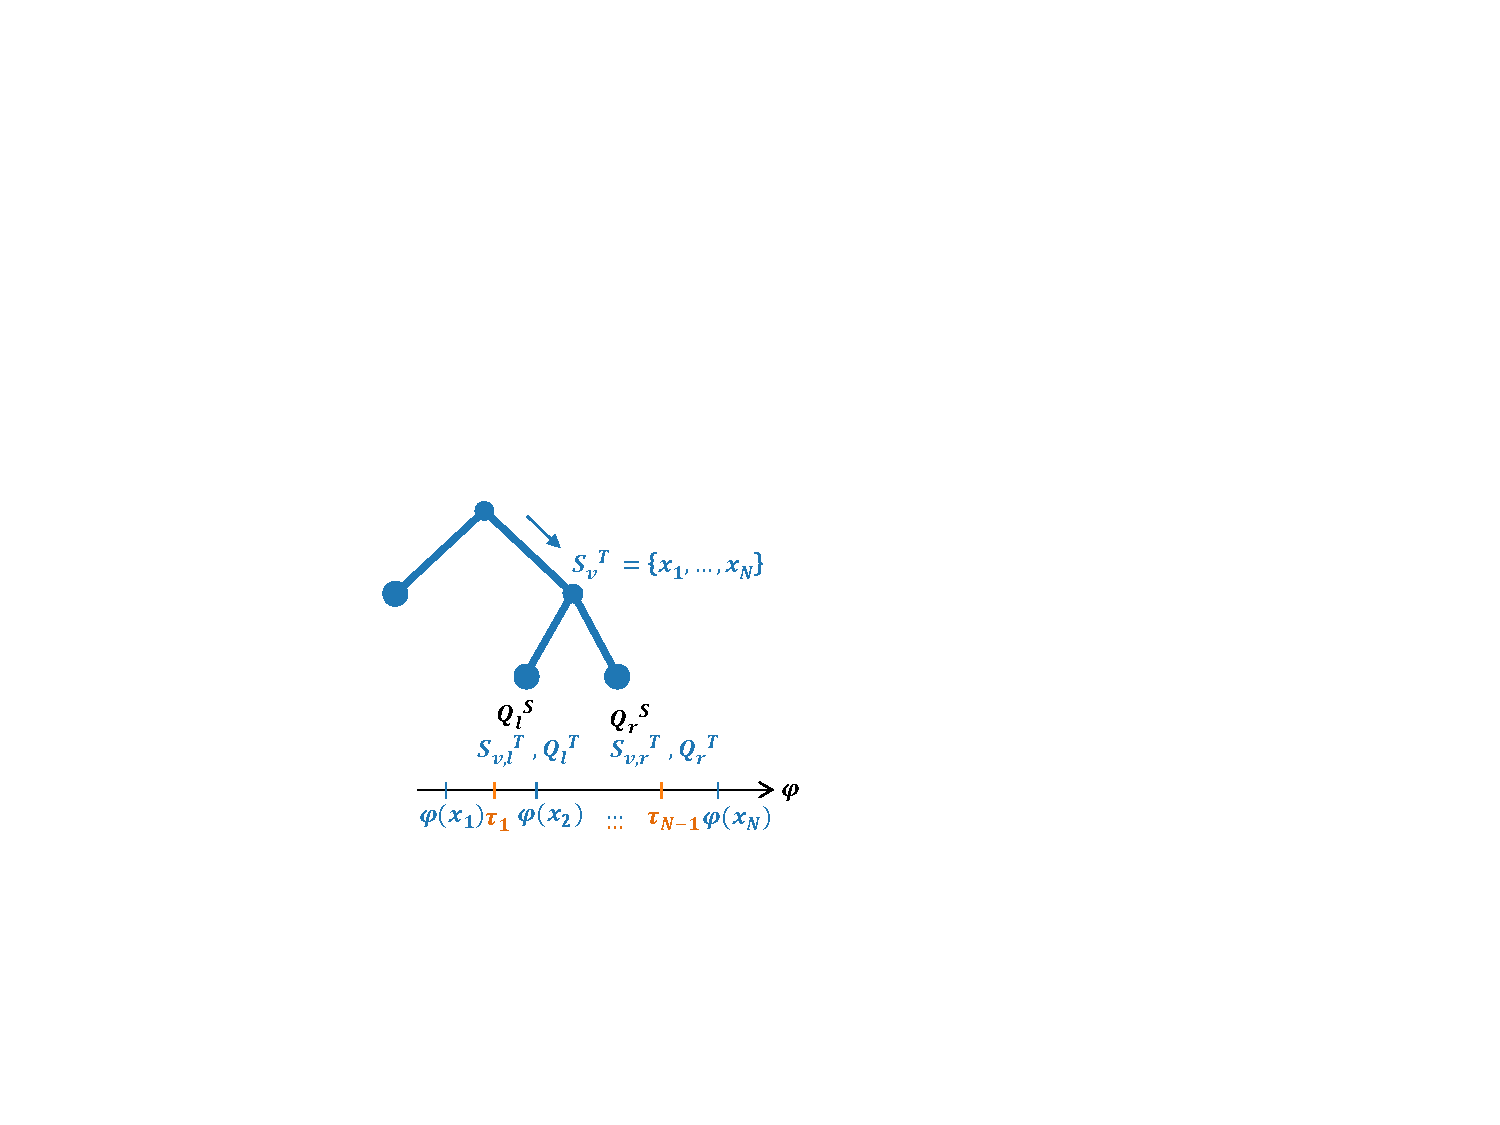
\includegraphics[width=\ratio\linewidth, trim={150 120 320 200}, clip]{schemas_strutoptim_5_15.pdf}
    \end{overprint}
\end{minipage}\hfill
\begin{minipage}[t]{0.55\linewidth}
    \vspace{0pt}
    
    \textbf{Goal: } Maximize DG while being in a local maximum of Information Gain (IG) (here IG = Gini gain)
    \pause \pause \pause
    \begin{align*}
        &\tau_{m} = \argmax_{\tau \in \mathrm{T}_{v}}\left(DG\left(  \tau ,  Q_{l}^{T}(\tau), Q_{r}^{T}(\tau)\right)\right) \\
        &\text{s.t.\ } IG(\tau_{m-1}) < IG(\tau_{m}) \text{ and } IG(\tau_{m}) > IG(\tau_{m+1})
    \end{align*}
    \vspace{1cm}

    \pause
    \begin{itemize}
        \item  $Q^S$ have less meaning when going deeper
        \item  Do we really want to keep $Q^S$ and $Q^T$ close ?
    \end{itemize}
\end{minipage}

\end{frame}

\begin{frame}{Introduction}{}
\begin{itemize}
    \item \textbf{Issue}: one-dimensional signals for large areas
    \item Goal: Classify elderly from other individuals
%     using a convolutional neural network 
    \begin{itemize}
        \item Most signals are made of walks of staff individuals
    \end{itemize}
    \item \textbf{Subtask}: Bring the model's attention over step-related signals
\end{itemize}
\begin{itemize}
    \item A model to recognize steps ?
\end{itemize}

\pause
\begin{figure}[h]
    \begin{minipage}{\linewidth}
        \centering
        \begin{minipage}{0.49\linewidth}
            \centering
            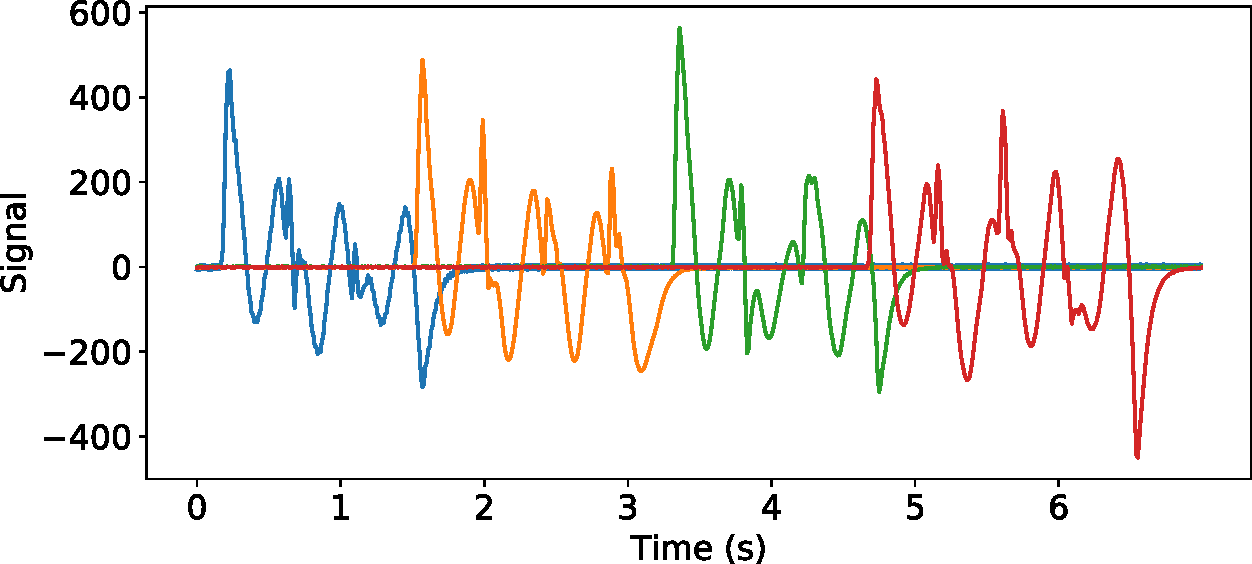
\includegraphics[width=0.9\linewidth]{signal_walk_young_female_before_preproc_2.pdf}\\
            {\small (a)\; Raw signal}
        \end{minipage}
        \begin{minipage}{0.49\linewidth}
            \centering
            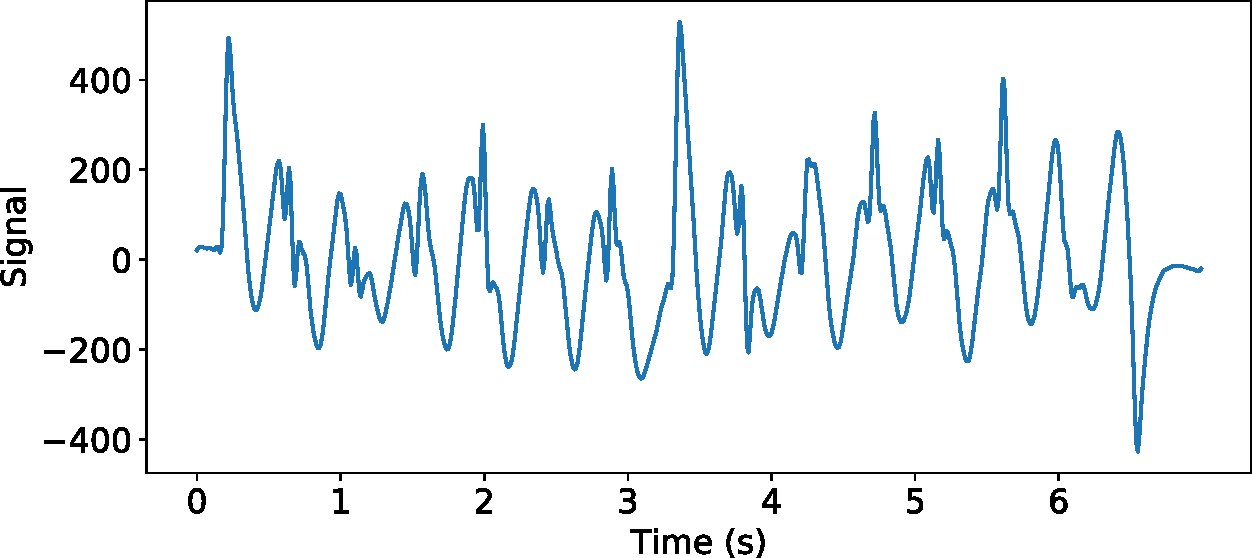
\includegraphics[width=0.9\linewidth]{signal_walk_young_female_after_preproc_2.pdf}\\
            {\small (b)\; Preprocessed signal}
        \end{minipage}
    \end{minipage}
    \caption{Healthy individual walking on the sensor.}
%     \label{fig:walk_class_ex_preprocessing}
\end{figure}
\begin{itemize}
    \item Signals are complex
    \item How to \textbf{localize} steps ?
    \item \textbf{This presentation:} A step detector using convolutional neural network: Step Proposal Network
\end{itemize}

\end{frame}
%
% ---------------------------------------------------------------
\section{Step proposal network}

% \subsection{Architecture}

\subsection{Region proposal network}

% \begin{frame}[noframenumbering]{\ }
% \hfill
% \parbox[t]{.85\textwidth}{
%   \begin{minipage}[c][0.65\textheight]{\textwidth}
%   \tableofcontents[currentsection, subsectionstyle=show/shaded/shaded]
%   \end{minipage}
% }
% \end{frame}


\begin{frame}{Region proposal network}{Object detection}
\begin{itemize}
    \item Classification: What is the image class ?
    \pause
    \item Object detection: Where are the objects and what are they classes ?
    \pause
    \item How to efficiently localize objects ?
    \item Proposal models \cite{hosang2016what}
    \item Faster R-CNN \cite{ren2015faster}
\end{itemize}
\begin{figure}
    \onslide<1->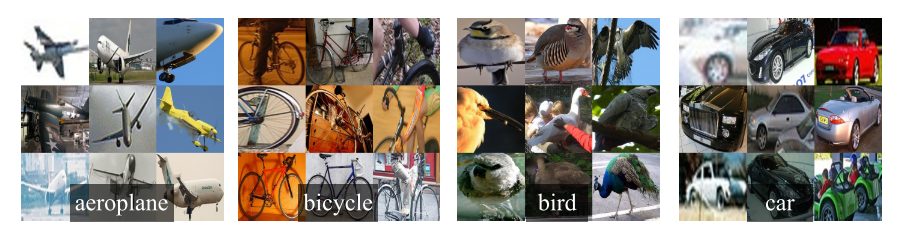
\includegraphics[width=\ratio\linewidth, trim=0 0 340 0, clip]{rcnn_images.png}
    \onslide<2->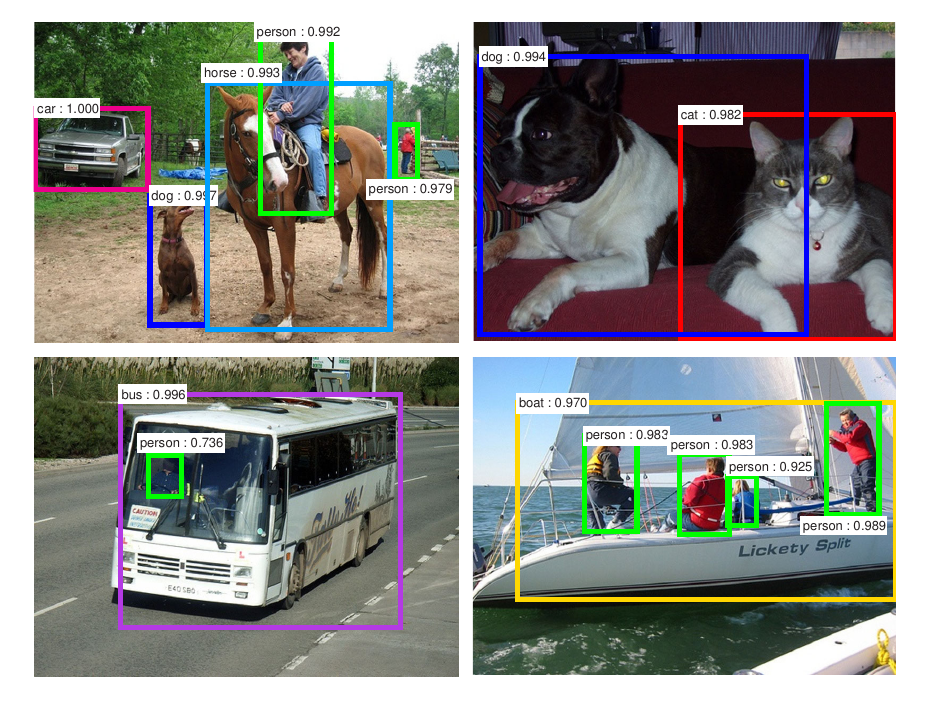
\includegraphics[width=\ratio\linewidth]{faster_rnn_rpn_imageoutputs.png}
    \onslide<1->\caption{Classification vs Object detection. Source: \cite{girshick2014rich},  \cite{ren2015faster}}
\end{figure}

\end{frame}

\begin{frame}{Region proposal network}{Faster R-CNN}
\begin{itemize}
    \item Main idea: proposals are generated by a CNN called Region Proposal Network
    \pause
    \item A sliding window is passed: multiple \emph{anchors} over each location (various sizes and scales)
    \item Two layers: Classification (Object / Not Object) and Regression (anchor coordinates)
\end{itemize}
    
\renewcommand{\ratio}{0.45}
\centering
\begin{figure}
    \onslide<1->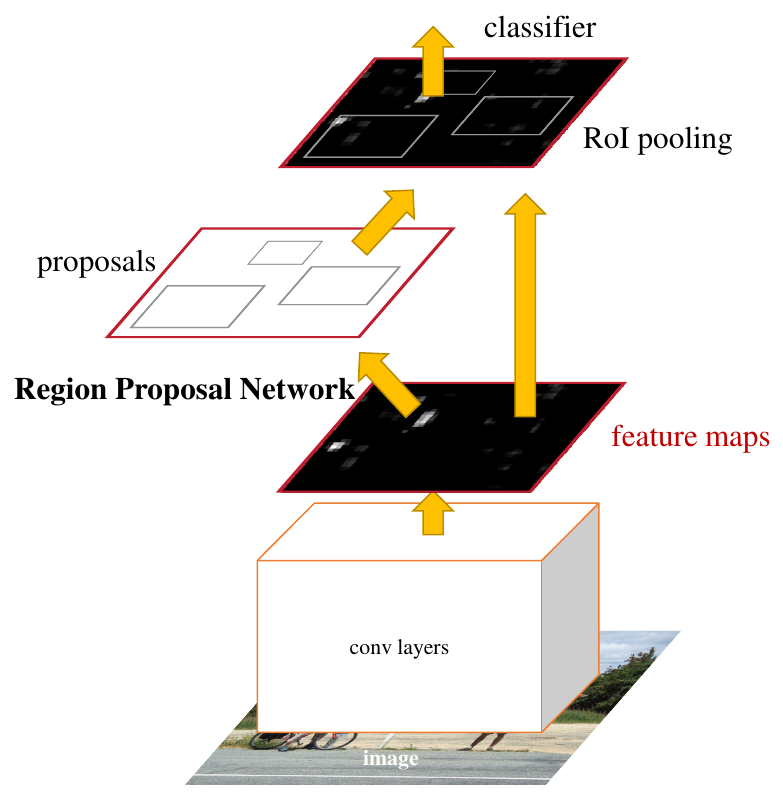
\includegraphics[width=0.4\linewidth]{faster_rnn_wholenetwork.png}
    \onslide<2->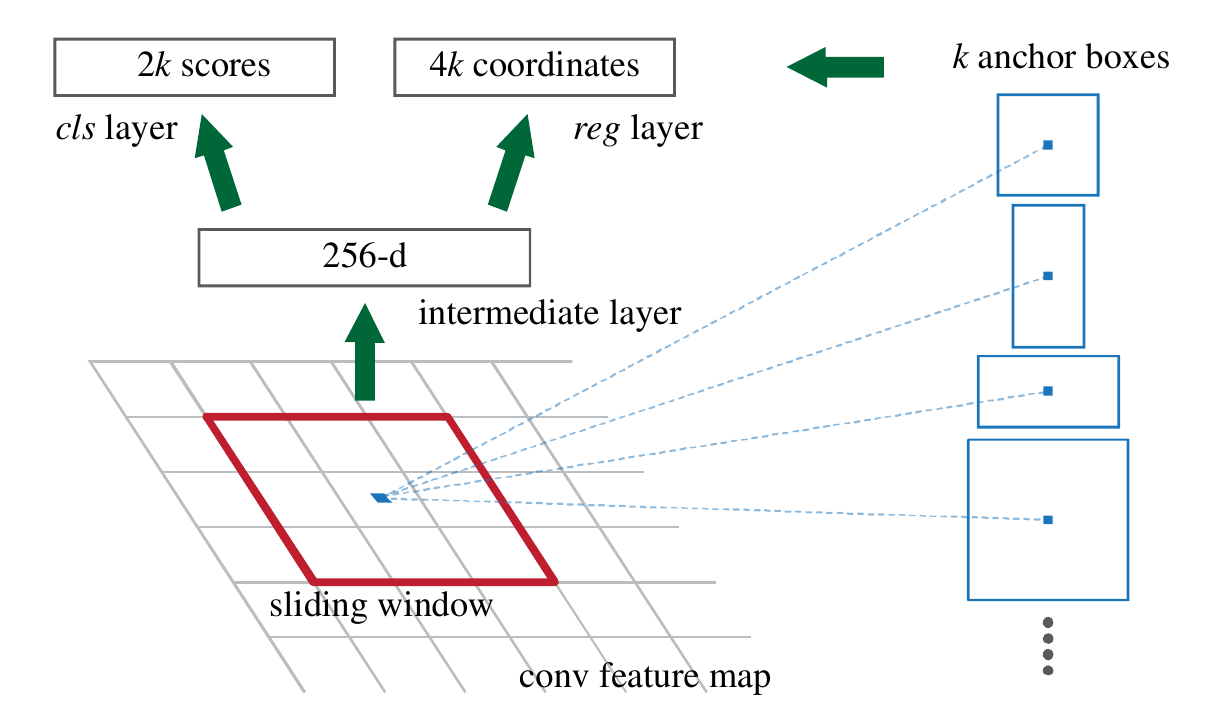
\includegraphics[width=0.55\linewidth]{faster_rnn_rpn.png}
    \onslide<1->\caption{Region proposal network. Source: \cite{ren2015faster}}
\end{figure}

\end{frame}

\subsection{Main architecture}

% \begin{frame}[noframenumbering]{\ }
% \hfill
% \parbox[t]{.85\textwidth}{
%   \begin{minipage}[c][0.65\textheight]{\textwidth}
%   \tableofcontents[currentsection, subsectionstyle=show/shaded/shaded]
%   \end{minipage}
% }
% \end{frame}

\begin{frame}{Step proposal network}{Main architecture}

\begin{itemize}
    \item Directly inspired from RPN
    \item Simple architecture with three hidden layers, all \textbf{convolutional}
    \item Output: probability of having a step at a specific window location and size
    \begin{itemize}
    \item Here 3 sizes and all discrete locations are considered
    \end{itemize}
\end{itemize}

\begin{figure}[h]
    \begin{minipage}{\linewidth}
        \centering
        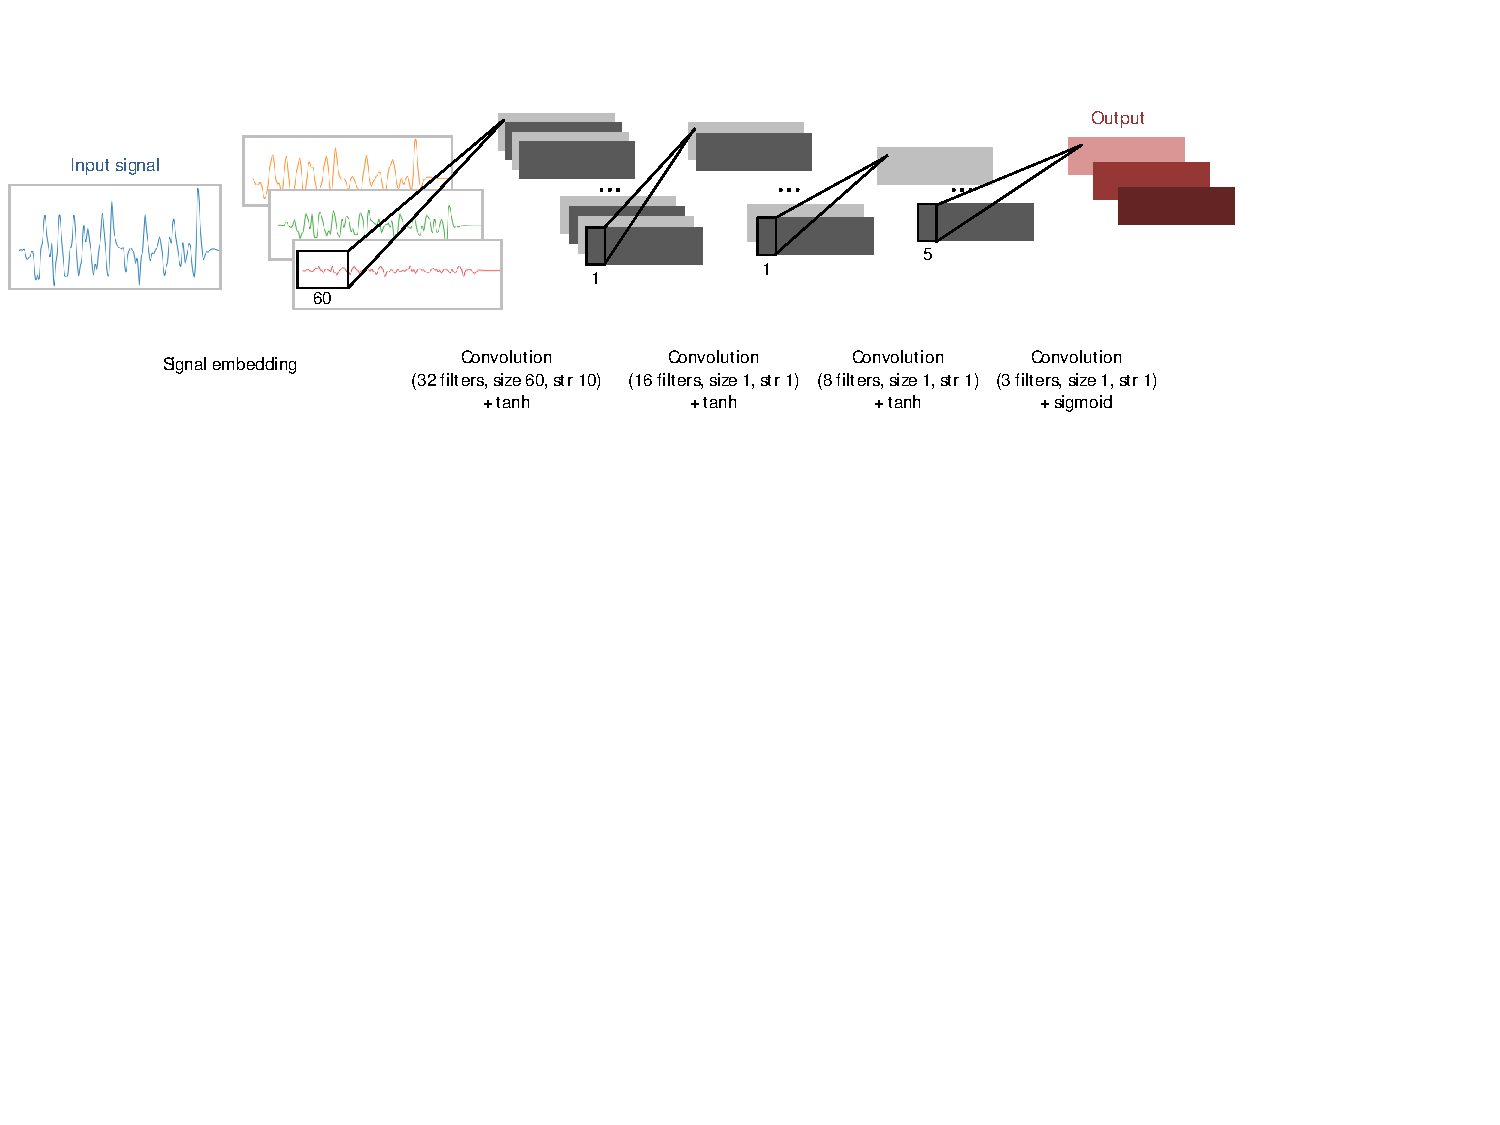
\includegraphics[width=\linewidth, trim= 0 340 120 40, clip]{schema_cnn_rpn}
        \caption{Architecture of \subalgo.}
%         \label{fig:walk_class_cnn_spn}
    \end{minipage}
\end{figure}

\pause
\begin{itemize}
    \item Use the convolutional representation to ``boost'' training
    \item First layer (Signal embedding) of \subalgo is trained \textbf{separately} using convolutional dictionary learning
\end{itemize}
    
\end{frame}

\subsection{Signal embedding}

% \begin{frame}[noframenumbering]{\ }
% \hfill
% \parbox[t]{.85\textwidth}{
%   \begin{minipage}[c][0.65\textheight]{\textwidth}
%   \tableofcontents[currentsection, subsectionstyle=show/shaded/shaded]
%   \end{minipage}
% }
% \end{frame}


\begin{frame}{Signal embedding}{Convolutional dictionary learning}
\begin{minipage}[t]{0.45\linewidth}
    \begin{itemize}
        \item $\bfs$ : data to be represented
        \item Objective : find $M$ atoms $\bfd_m$ and activation signals $\bfx_m$ such that
        $$\bfs \approx \sum_{m=1}^{M}\bfx_m * \bfd_m$$
        \item $*$ : convolution
    \end{itemize}
    \pause[3]
    CDL general problem:
    \begin{gather*}\label{eq:cdl_baseform}
    \argmin_{\bfx_m,\bfd_m} \frac{1}{2} \left\| \sum_{m=1}^{M} \bfx_{m} * \bfd_m - \bfs \right\|_2^2 + \lambda \sum_{m=1}^{M} \|\bfx_m \|_1 \ \\
        \text{s.t.}\quad \| \bfd_m\|_2 \leq 1 \quad \forall m \;. \nonumber
    \end{gather*}
\end{minipage}\hfill
\begin{minipage}[t]{0.4\linewidth}
    \centering
    \pause[2]
    \begin{figure}[h]
        \centering
        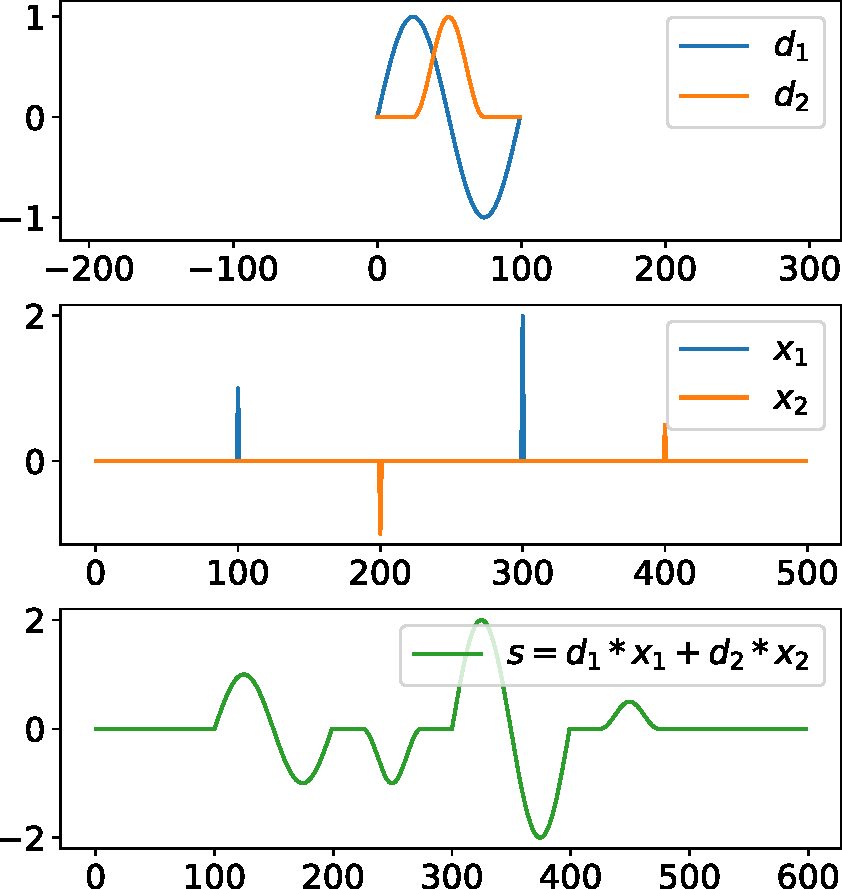
\includegraphics[width=0.9\linewidth]{cdl_example_2.pdf}\\
        \caption{Convolutional dictionary learning.}
%         \label{fig:walk_class_ex_stepboxes}
    \end{figure}
\end{minipage}

\end{frame}

\begin{frame}{Signal embedding}{Learning step atoms}

\renewcommand{\ratio}{0.9}
\centering
\begin{minipage}[t]{0.45\linewidth}
\begin{itemize}
    \item Learning with Alternating Direction Method of Multipliers (ADMM) \cite{bristow2013fast}
%     \begin{itemize}
        \item 3 atoms of length 0.7 second
%     \end{itemize}

    \pause[3]
    \item Use the following embedding:
\begin{equation*}\label{eq: convolutional embedding}
\bfS \doteq \Big( \bfs * \bfd_m\Big)_{1 \le m \le 3 }
\end{equation*}
        
\end{itemize}

    \centering
    \begin{figure}
    \onslide<1->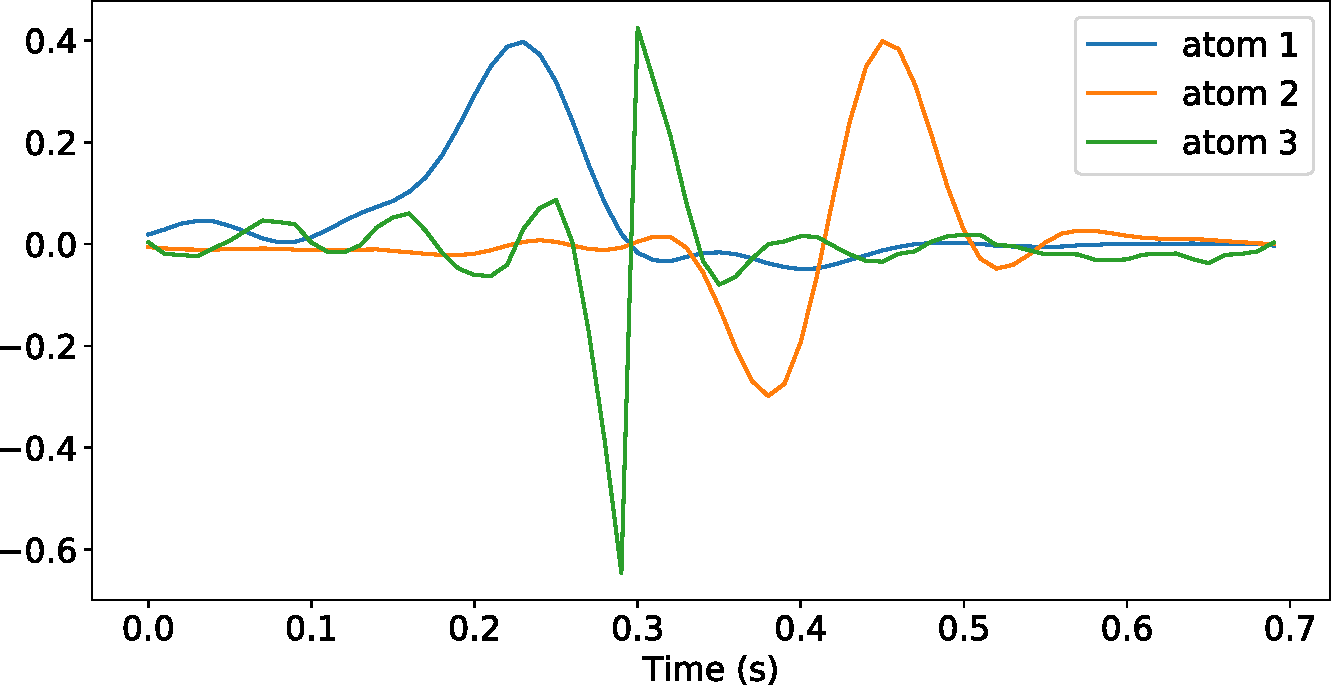
\includegraphics[width=0.85\linewidth]{dictionary.pdf}
%     \caption{Dictionary.
%         Note that the amplitude of the atoms is small compared to the signal due to the fact that they are normalized in the training process.}
    \caption{Dictionary.}
    \end{figure}
\end{minipage}
\begin{minipage}[t]{0.54\linewidth}
    \pause
    \begin{figure}
        \begin{minipage}{\linewidth}
            \centering
            \onslide<2->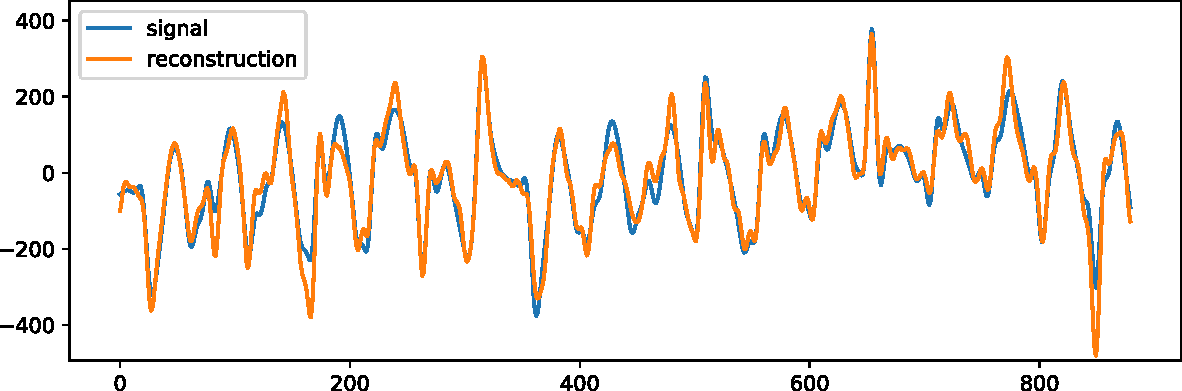
\includegraphics[trim= 0 0 0 0, width=\ratio\linewidth, clip]{signal_walk_young_female_csc_1.pdf}\\
            {\small (a)\; Original signal and its reconstruction}
        \end{minipage}\\
        \begin{minipage}{\linewidth}
            \centering
            \onslide<2->\includegraphics[trim= 0 0 0 0, width=\ratio\linewidth, clip]{signal_walk_young_female_csc_2.pdf}\\
            {\small (b)\; Signal activations}
        \end{minipage}\\
        \begin{minipage}{\linewidth}
            \centering
            \onslide<3->\includegraphics[trim= 0 0 0 0, width=\ratio\linewidth, clip]{signal_walk_young_female_csc_3.pdf}\\
            {\small (c)\; Embedding}
        \end{minipage}
        \onslide<2->\caption{Signal encoding and embedding.}
    \end{figure}
\end{minipage}

\end{frame}



\subsection{Step proposal network}

% \begin{frame}[noframenumbering]{\ }
% \hfill
% \parbox[t]{.85\textwidth}{
%   \begin{minipage}[c][0.65\textheight]{\textwidth}
%   \tableofcontents[currentsection, subsectionstyle=show/shaded/shaded]
%   \end{minipage}
% }
% \end{frame}


\begin{frame}{Step proposal network}{Principle}

\begin{minipage}{0.7\linewidth}
    \begin{itemize}
        \item Objective of \subalgo: output boxes with largest Intersection over Union ($\iou$)
        \item $\iou$: $\mathbf{b_j}$ are labelled boxes, $\hat{b}$ is an estimated box:
    \begin{equation*}\label{eq: def IOU}
    \iou(\hat{b}) \doteq \max_{j} \frac{ \vert \mathbf{b_j} \cap \hat{b}\vert}{\vert \mathbf{b_j} \cup \hat{b}\vert}
    \end{equation*}
    \end{itemize}
\end{minipage}\hfill
\begin{minipage}{0.3\linewidth}
    \centering
    \includegraphics[width=0.7\linewidth]{iou_scheme.pdf}
\end{minipage}

\pause

\begin{figure}[h]
    \centering
    \begin{minipage}[t]{0.45\linewidth}
        \centering
        \includegraphics[width=0.6\linewidth]{example_step.pdf}\\
        {\small (a)\; Step signal}
    \end{minipage}\hfill
    \begin{minipage}[t]{0.55\linewidth}
        \centering
        \includegraphics[width=\linewidth]{signal_walk_young_female_stepboxes.pdf}\\
        {\small (b)\; Step labels over a walk signal}
    \end{minipage}
    \caption{Example of a typical step (a) and true steps delimiting boxes in a walk signal (b).}
%     \label{fig:walk_class_ex_stepboxes}
\end{figure}
\end{frame}

\begin{frame}{Step proposal network}{Training}
\begin{itemize}
    \item Output: a matrix $\mathbf{W} \in \mathbb{R}^{T \times K}$
    \begin{itemize}
        \item $T$: signal length
        \item $K$: number of different box sizes
    \end{itemize}

    \item $\mathbf{W}_{t,k}$: probability that the box $b_t^k$ starting at time $t$ and of size $0.4$s, $0.5$s, or $0.6$s (for respectively $k=1$, $2$, or $3$) has a large $\iou$ score
    \item Positive boxes: $\iou(b_t^{k}) > \sqrt{0.7}$
    \item Negative boxes: $\iou(b_t^{k}) < \sqrt{0.3}$
    \item Other are not used for training
\end{itemize}

\vspace{0.8cm}

The loss function $\mathcal{L}$ over a signal $\bfs$ is defined as:
\begin{equation*}\label{eq: loss training CNN}
\mathcal{L}(\bfs, \mathbf{W}) = \sum_{t} \sum_{k \in \left[1, 2, 3 \right]} \bbmind_{ \iou(b_t^{k})> \sqrt{0.7} } \log(\mathbf{W}_{t,k}) + \bbmind_{ \iou(b_t^{k})< \sqrt{0.3} } \log(1-\mathbf{W}_{t,k}). 
\end{equation*}
\end{frame}

\subsection{Results}

% \begin{frame}[noframenumbering]{\ }
% \hfill
% \parbox[t]{.85\textwidth}{
%   \begin{minipage}[c][0.65\textheight]{\textwidth}
%   \tableofcontents[currentsection, subsectionstyle=show/shaded/shaded]
%   \end{minipage}
% }
% \end{frame}


\begin{frame}{Results}
\begin{minipage}[t]{0.45\linewidth}
    Data
    \begin{itemize}
        \item 43 signals recorded in a nursing home
        \item Manually labeled steps
    \end{itemize}
    Training
    \begin{itemize}
        \item \subalgo is trained using classical gradient descent
        \item Training time: < 5 minutes
        \item Inference (detection over a 10s signal): < 1 second
        \item Optimization details
        \begin{itemize}
            \item learning rate of $10^{-3}$
            \item learning rate decay ($\times 0.9$ every 10 epochs)
            \item Nesterov momentum
        \end{itemize}
    \end{itemize}
\end{minipage}\hfill
\begin{minipage}[t]{0.5\linewidth}
    \begin{figure}[h]
    %     \begin{minipage}{\linewidth}
            \centering
            \includegraphics[width=\linewidth]{spn_train_test_errors.pdf}
    %     \end{minipage}
        \caption{\subalgo training and testing errors.}
    %     \label{fig:walk_class_spn_detection_test_example}
    \end{figure}
\end{minipage}
\end{frame}

% \begin{frame}{Results}
% \begin{figure}[h]
%     \begin{minipage}{\linewidth}
%         \centering
%         \includegraphics[width=0.75\linewidth]{SPN_Mercredi_11_28_01_00_to_11_28_08_90.pdf}
%     \end{minipage}
%     \caption{Test of \subalgo over a walk signal.}
%     \label{fig:walk_class_spn_detection_test_example}
% \end{figure}
% \end{frame}

\begin{frame}{Results}
% \animategraphics[loop,controls,width=\linewidth]{2}{Mercredi_10_19_13_00_to_10_19_18_85_th_}{1}{4}
% \animategraphics[loop,controls,width=\linewidth]{2}{test_}{1}{4}
\begin{itemize}
    \item Object detection use the mean Average Precision (mAP): area under the Precision-Recall curve
    \item \textbf{Without} embedding, mAP = 72,5\%
    \item \textbf{With} embedding, mAP = 78,6\%
\end{itemize}
\pause

\begin{figure}[h]
    \begin{overprint}
        \onslide<2>\centering\includegraphics[width=0.75\linewidth]{Mercredi_10_19_13_00_to_10_19_18_85_th_005.pdf}
        \onslide<3>\centering\includegraphics[width=0.75\linewidth]{Mercredi_10_19_13_00_to_10_19_18_85_th_02.pdf}
        \onslide<4>\centering\includegraphics[width=0.75\linewidth]{Mercredi_10_19_13_00_to_10_19_18_85_th_03.pdf}
    \end{overprint}
    \caption{Test of \subalgo over a walk signal.}
\end{figure}
\end{frame}

\section{Conclusion}
\subsection{}

\begin{frame}{Conclusion}

% \vspace{1cm}
\centering
\begin{minipage}[t]{0.8\linewidth}
Conclusion
\begin{itemize}
    \item SPN uses the convolutional representation to detect steps
    \item Allows to located steps in complex signals
    \item Training and inference are fast
\end{itemize}
Future work
\begin{itemize}
    \item Add a regression layer on the step proposals
    \item Tests on step detection benchmarks data sets
\end{itemize}
\end{minipage}

\vfill
\pause
% \vspace{1cm}
\begin{block}{\centering Thanks}
\medskip
Contact: minvielle@cmla.ens-cachan.fr\\[5pt]
Reference: L. Minvielle and J. Audiffren. Nursenet : Monitoring elderly levels of activity with a
piezoelectric floor. Sensors, 19(18), 2019
\; \href{https://www.mdpi.com/1424-8220/19/18/3851}{{\usebeamercolor[fg]{structure} link}}
\end{block}
\end{frame}
